%\graphicspath{{../img/experiments/}}
\chapter{OIGAS: an Optimized Incremental
Insertion-Based Graph for Efficient Vector Search}
\chaptermark{OIGAS: a New Base Graph for ELPIS+}
\label{chapter:oigas}
ELPIS+ exploits a hybrid approach combining both tree and graph structures for approximate vector search, demonstrating how it successfully scales to large datasets while adapting to both latency and throughput requirements. However, this approach depends on existing graph indexes, such as HNSW, to organize and search leaf nodes. Our next objective is to leverage the insights gained from our extensive experimental evaluation of twelve state-of-the-art graph-based indices to design a graph-based index tailored for ELPIS+ that can further enhance both indexing and search performance.
%In particular: We propose 
%In this chapter, we present various experiments conducted on the incremental insertion-based graph HNSW, which we employ for the leaf nodes. We show that certain techniques used in recent graph-based approaches do not necessarily improve graph performance. We propose 
%a novel approach, called Step-Wise Adaptive Beam Width (SWB), for constructing incremental insertion graphs; %for efficiently building these graphs for vector search. 
%2) we introduce a combination of ND strategies to enhance search efficiency; and 3) we optimize both indexing and search performance with the adoption of a single priority queue to track promising nodes and their expansions, rather than using two priority queues as in HNSW. \karima{???Make sure chapter is organized according to these 3 main ideas???} 

This chapter details the incremental insertion construction paradigm of HNSW and introduces two optimizations: Step-wise Adaptive Beam Width (SWB) for efficient graph building, and a combined Neighborhood Diversification (ND) strategy during indexing to enhance search efficiency. We evaluate these optimizations on incremental insertion-based graphs alongside techniques such as using visited nodes as candidate neighbors, single priority queue beam search, and k-sampling seed selection. Finally, we integrate all efficient techniques into an optimized incremental insertion graph-based vector search method, OIGAS, which we evaluate against state-of-the-art method for incremental insertion on indexing and search tasks using datasets up to 1 billion in size.

All improvements and experiments in this section are based on HNSW, the current state-of-the-art method for incremental insertion, as it demonstrates superior scalability and search performance compared to other methods that build and search a single graph structure.
\newpage
\section{Incremental Insertion Construction Paradigm}
NSW first introduced the incremental insertion paradigm to state-of-the-art methods, incrementally building the graph by inserting nodes one at a time, obtaining each node’s neighborhood by searching already-inserted nodes, and adding bidirectional edges to ensure connectivity regardless of insertion order. HNSW~\cite{hnsw} improved upon NSW by reducing the high number of distance calculations required during search. It applies RND diversification to prune edges during construction and introduces a lightweight, stacked NSW structure to identify the seed or entry node before performing beam search on the base graph containing all dataset points.
Algorithm ~\ref{alg:node_insertion} illustrates the general process of inserting a node during the construction of the II-based HNSW graph.
% \begin{figure}[tb] 
% \centering
% 		\captionsetup{justification=centering}
% 		\includegraphics[width=0.7\columnwidth]{../img/oigas/fasterbeamsearch_IIBASE.png}
% 		\caption{Node insertion in the HNSW graph during graph construction \karima{???This figure seems to not be referenced anywhere. Change to be an algorithm or remove it if not needed???}}        
% 		\label{fig:node_insertion}
%  \end{figure}

 \begin{algorithm}[htb]
\caption{Node Insertion into Graph $G'$}
\label{alg:node_insertion}
\begin{algorithmic}[1]
    \Require Graph $G'$, a new node $x$ and Beam width $L$
    \Ensure Updated graph $G'$ with new node
    \Statex
    \State $C_x \gets \text{BeamSearch}(G', x, L)$ 
    \State $R_x \gets \text{Prune}(C_x, MaxOut, strategy)$ 
    \ForAll{$y \in R_x$}
        \State $R_y \gets R_y \cup \{ x \}$ 
        \If{$|R_y| > MaxOut$}
            \State $R_y \gets \text{Prune}(R_y, MaxOut, strategy)$ 
        \EndIf
    \EndFor
\end{algorithmic}
\end{algorithm}
To insert a node \( x \) in the current graph \( G' \): first, run a beam search on \( G' \), which contains previously inserted nodes, using the current node as the query (Line 1). The beam width $L$, provided as an input parameter (denoted \( \text{efc} \) in HNSW~\cite{hnsw}), determines the \( L \) nearest neighbors to \( x \). Next, prune this list using a node diversification (ND) strategy—RND in the case of HNSW—to limit edges to only promising neighbors (Line 2). Then, we add bidirectional edges to the nearest neighbors of x (Lines 3, 4). If any neighbor exceeds the maximum outdegree (Line 5), we prune the neighbor’s connections using the same strategy (Line 6).

This process, adopted by HNSW, is similar to methods like NSG and Vamana, which prune an existing graph by running searches on a complete graph \( G \) of all data points, rather than a partial graph \( G' \). NSG and Vamana vary slightly in that they return the list of visited nodes during search as candidate neighbors instead of the \( L \) nearest neighbors. Additionally, Vamana applies a Relaxed Relative Neighborhood Diversification (RRND) in the pruning stages, while NSG ensures graph connectivity by constructing a DFS tree starting from the medoid and adding edges as needed to connect all nodes. This process is repeated until the graph is fully connected.

While these differences are noteworthy, the authors did not provide sufficient evidence of the impact of these modifications on graph performance~\cite{nsg,vamana}. Previously, we presented a study of various ND strategies and their effects on search performance. In the following chapter, we empirically evaluate how other modifications affect graph performance, specifically by using the set of visited nodes as candidate neighbors and employing multiple DFS runs to improve connectivity and reachability in graph search.

We introduce two new optimizations for the incremental insertion paradigm: Step-Wise Adaptive Beam Width (SWB) and combined ND approaches for different pruning stages. We also propose OIGAS, an Optimized Incremental Insertion Graph for Approximate Vector Search. In the next sections, we compare various incremental insertion approaches for graph-based methods, specifically HNSW, focusing primarily on distance calculations and comparisons with the original HNSW implementation~\cite{url/hnsw}.



\section{Adaptive Beam Width}
The top-performing graph-based approaches for vector search share common techniques, including the retrieval of candidate neighbors through beam search~\cite{hnsw,nsg,vamana,SPTAG4,elpis}.

To perform beam search~\cite{beamsearch}, specific inputs are required, notably the beam width. The beam width defines the size of the priority queue used during search to track promising nodes for expansion. This parameter manages the trade-off between efficiency and accuracy: higher beam width increases the number of visited nodes, comparisons, and ultimately accuracy.

The beam width is typically chosen based on dataset size and the required number of nearest neighbors. Similar to \( k \)-NN search, a higher beam width improves neighbor quality (increasing the probability of retrieving a high-recall neighbor list). Consequently, during graph construction, the beam width is set high enough to ensure candidate neighbors closely match the query node. 

Most ND approaches refine an existing graph by running a search for each node on a graph containing all data points. In contrast, incremental insertion (II)-based graphs such as NSW and HNSW search on a subset of nodes. Earlier nodes generally require a smaller priority queue than later nodes, which search in a larger graph, leading to unnecessary computations in II-based graphs.

A straightforward solution is to linearly adjust the beam width with the current graph size. Given a maximum graph size \( S \) and an optimal beam width \( L \), each new node \( i \) inserted into the current graph \( G' \) of size \( S' \) would use an adapted beam width \( L' = \frac{S' \times L}{S} \).
\begin{figure}[htbp]
    \centering
    \captionsetup{justification=centering}
	\centering
		\captionsetup{justification=centering}
		\captionsetup[subfigure]{justification=centering}
        \begin{subfigure}[b]{\textwidth}
        \centering
 		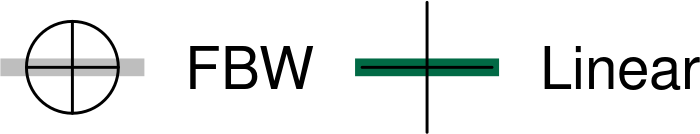
\includegraphics[width=0.3\columnwidth]{../img/oigas/Linear/legend.png}
    \end{subfigure}
    
            \begin{subfigure}[b]{0.3\textwidth}
            \centering
                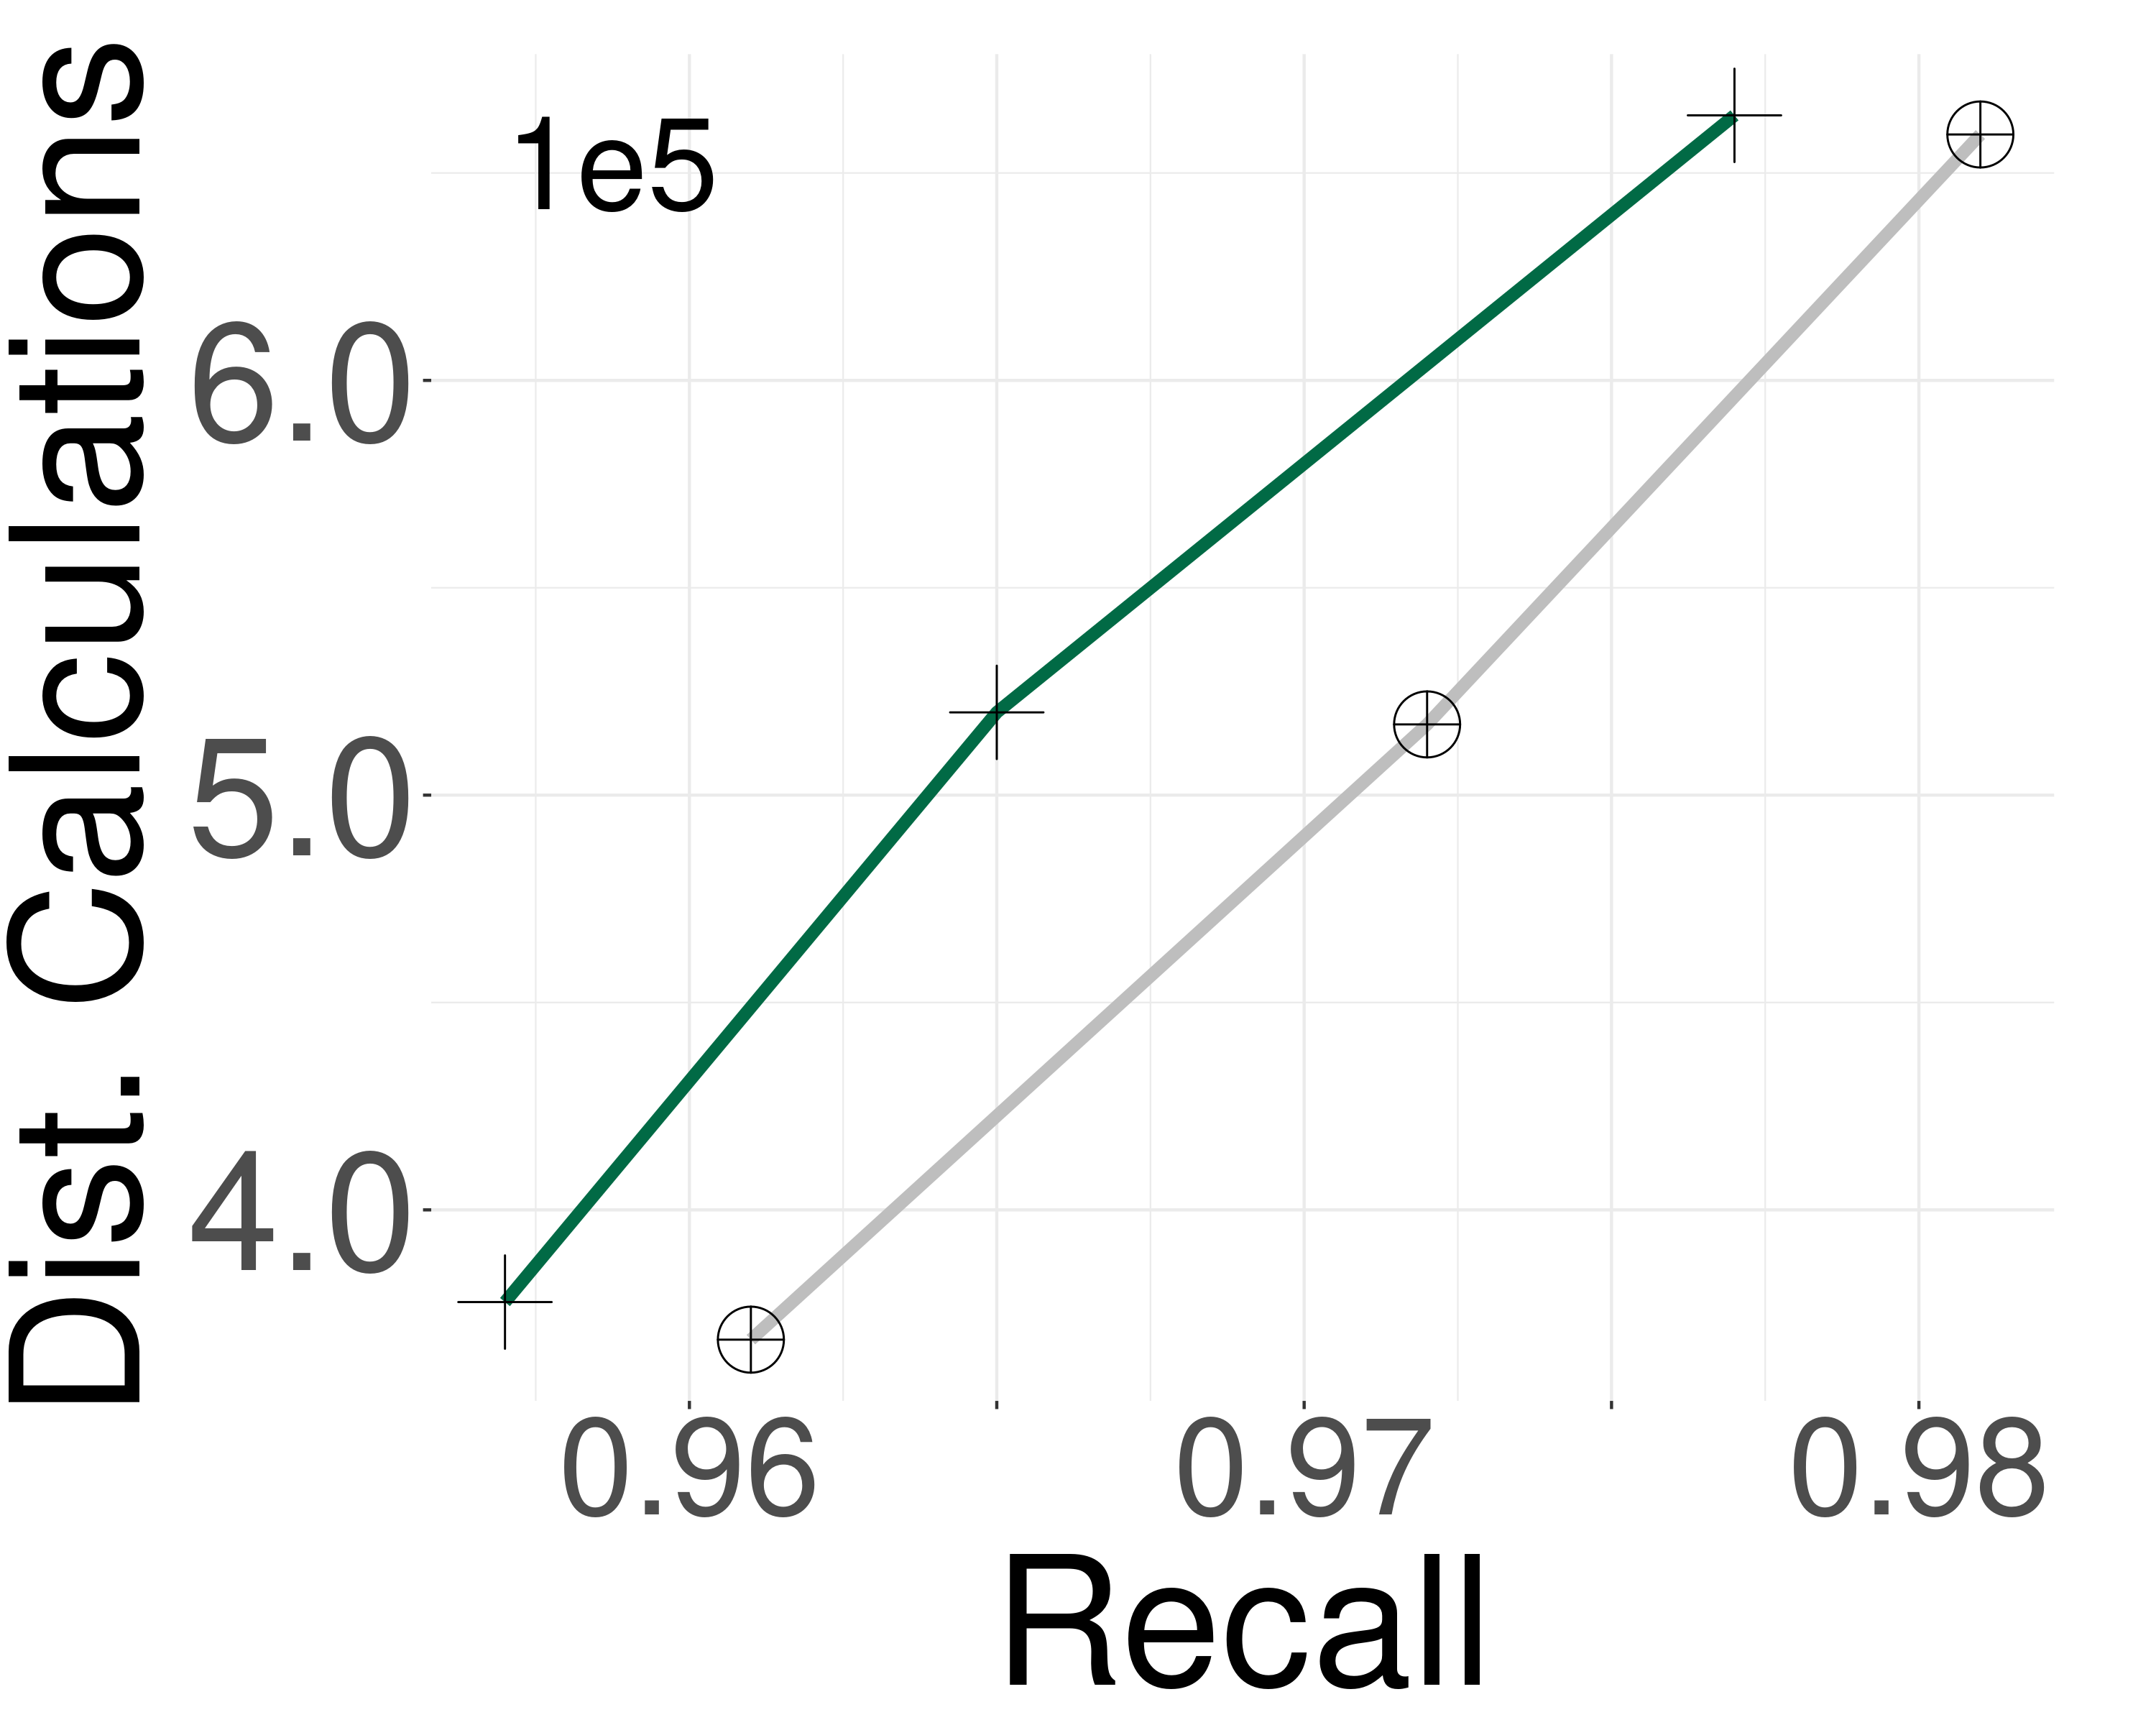
\includegraphics[width=\textwidth]{../img/oigas/Linear/deep_DC.png}
        \caption{Deep}
        \label{fig:oigas:linear:deep}
    \end{subfigure}
    \hspace{0.4cm}
             \begin{subfigure}[b]{0.3\textwidth}
                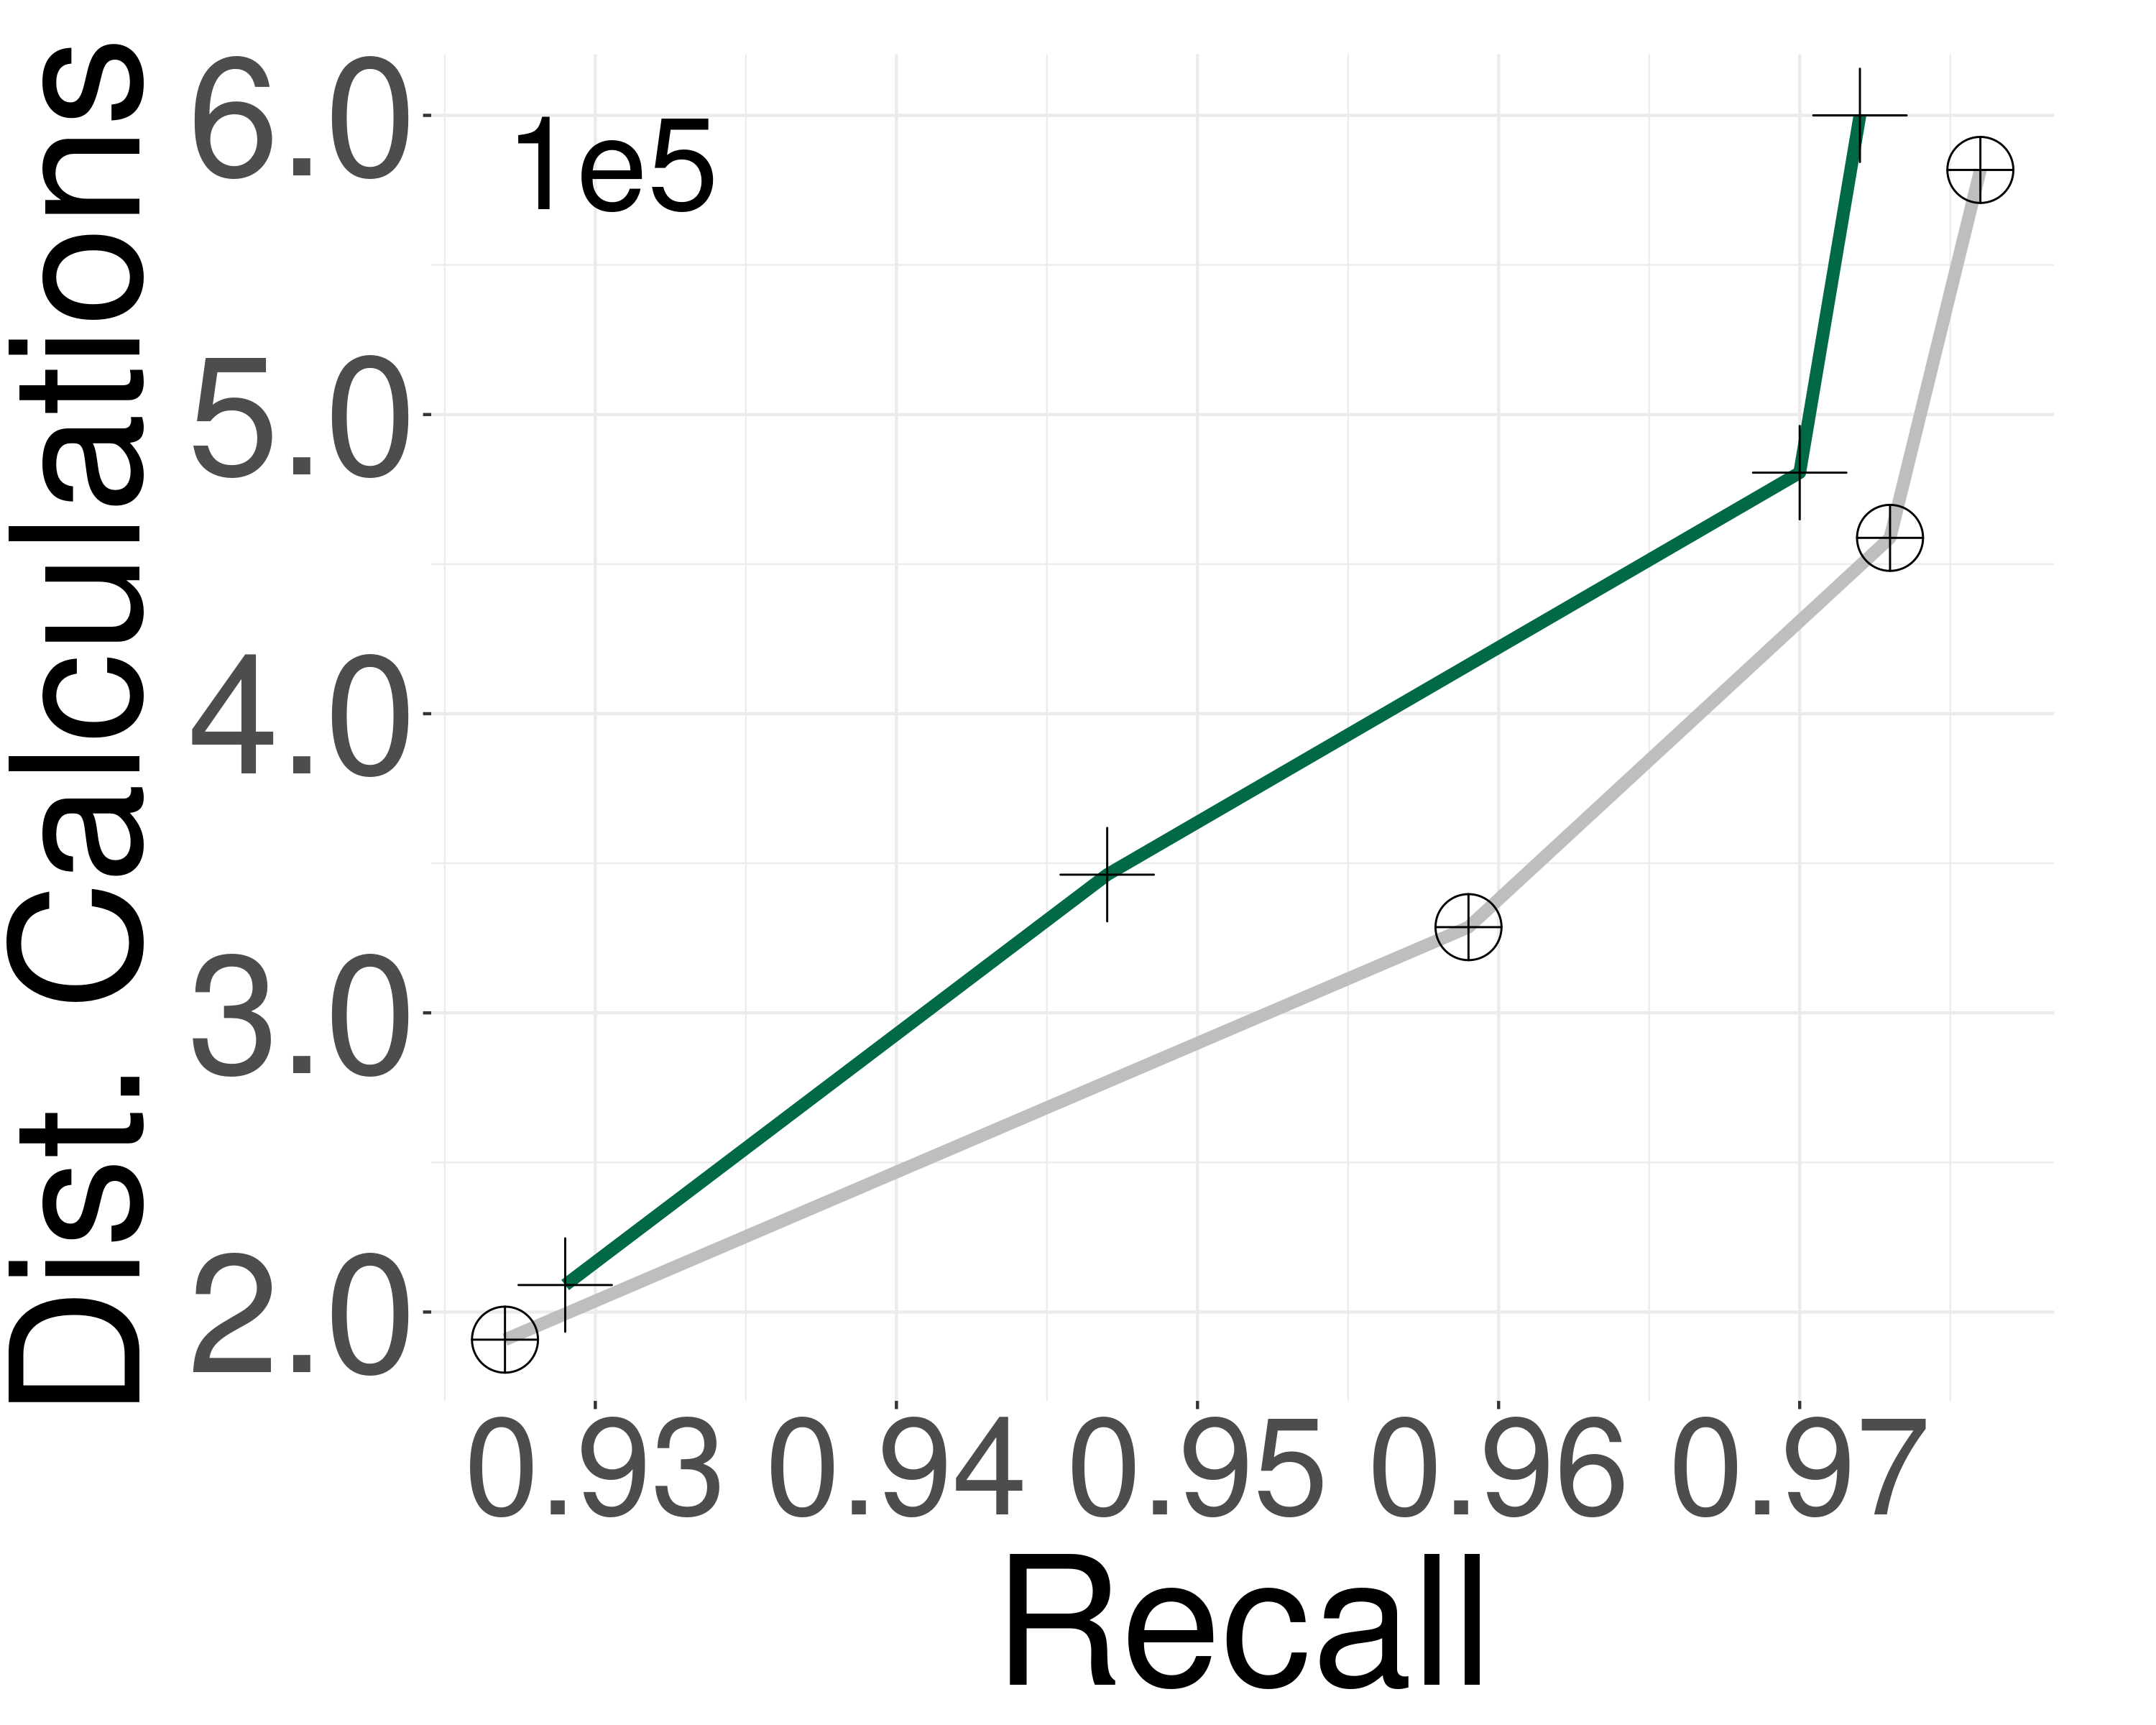
\includegraphics[width=\textwidth]{../img/oigas/Linear/sift_DC.png}
        \caption{Sift}
        \label{fig:oigas:linear:sift}
    \end{subfigure}

    \caption{Search Performance on 25GB datasets}
    \label{fig:oigas:linear}
\end{figure}


However, as shown in Figure~\ref{fig:oigas:linear}, this linear approach can degrade search performance. This is mainly because the relationship between optimal beam width and graph size is logarithmic rather than linear.

These findings motivate the development of an adaptive approach to dynamically adjust the beam width during each node insertion without compromising search performance or increasing indexing overhead. The following section introduces Step-wise Adaptive Beam Width (SWB), which incrementally adjusts the beam width for each inserted node based on the current graph size.

\subsection{Step-Wise Adaptive Beam Width}
Step-Wise Adaptive Beam Width (SWB) dynamically adjusts the beam width \( L_i \) during the incremental insertion of nodes based on the current graph size. The algorithm calculates a \textit{step index}, representing the relative position of the current graph size within the total dataset size \( N \), scaled by a factor \( \alpha \). This step index divides the graph into segments, or "steps," of equal size, which determines the beam width for each range of graph sizes. If the step index exceeds the maximum allowable value, it is capped at \( \alpha - 1 \). 

The beam width \( L_i \) is then adjusted by scaling this step index relative to the maximum beam width \( L \). This stepwise approach ensures that \( L_i \) adapts incrementally as the graph grows, optimizing the insertion process by balancing computational efficiency with the accuracy of neighbor selection.


\begin{algorithm}
\caption{Step-wise Adaptive Beam Width}
\label{alg:sba}
\begin{algorithmic}[1]
\Require size, $N$, $\alpha$, $MaxL$
\Ensure Adapted $L$ value

\State $step\_size \gets \frac{MaxL}{\alpha}$ \Comment{Divide Beam width by number of steps}
\State $step\_index \gets \min(\alpha - 1, \lfloor \frac{\text{size}}{step\_size} \rfloor)$ \Comment{Calculate capped step index}
\State $L \gets \frac{step\_index}{\alpha - 1} \times MaxL$ \Comment{Adapt $L$ based on step index}

\State \textbf{return} $L$
\end{algorithmic}
\end{algorithm}


% \begin{algorithm}[H]
% \caption{SBA Algorithm}
% \label{alg:sba}
% \KwIn{size, $N$, $\alpha$, $MaxL$}
% \KwOut{Adapted $L$ value}

% $step\_size \gets \frac{N}{\alpha}$ \tcp{Split size across the number of steps}
% $step\_index \gets \min\left(\alpha - 1, \left\lfloor \frac{\text{size}}{step\_size} \right\rfloor\right)$ 
% \tcp{Determine step index, capped by $\alpha - 1$}

% $L \gets \frac{step\_index}{\alpha - 1} \times MaxL$ \tcp{Adapt $L$ based on the current step}
% \Return $L$\;

% \end{algorithm}

\section{Combined ND approaches}
Graph approaches apply pruning strategies in two stages: (1) After retrieving the candidate neighbors of a node with beam search (Line 2 in Alg.3). (2) When the size of a node's neighborhood list exceeds the maximum outdegree due to the addition of bidirectional edges from other nodes (Line 6 in Alg.3). 

A node that has been pruned in stage 2 pruning, will probably have more in-coming edges. %(due to nodes inserted m afterwards inserted nodes that connect with biderectionl edges casuing previous inserted nodes outdegree to exceed the threshold). 
Thus the probability of visiting this set of nodes during the graph search is higher. 

%Our next intuition is to use
We propose to use different pruning approaches for both pruning stages (1) and (2).
%while we have no prior guanrantee that a node will have a high in-degree during its insertion, when a node neighborhood list is pruned in stage 2, this give us the insight that such nodes will have a higher in-degree than the later \karima{???rephrase sentence. Not clear???}. 
Our idea is to relax the second pruning of nodes which have a higher probability to be visited during search. This is because these nodes will propose more direction during routing and thus facilitate the convergence of the search to interesting regions in the graph. 

We then adapt a combination of ND approaches during indexing. In stage 1 pruning, we prune all nodes using the RND approach. During the second pruning phase, we adopt RRND to allow the node to prune fewer neighbors. This results in nodes keeping more edges. thus facilitating the routing during search as these nodes have a higher in-degree. In the experimental section 7.4.4, we will show how this approach reduces number of distance calculations during query answering on the graph.



\section{OIGAS: Optimized Incremental
Insertion-based Graph for Efficient
Vector Search}
In this section, we evaluate the steps adopted in different graph-based methods that can be integrated into our new Incremental Insertion (II) base model and assess their effectiveness. Additionally, we propose enhancements to improve the indexing and search efficiency of II-based graph, specifically Step-wise Adaptive Beam Width (SWB) and Combined Neighborhood Diversification (Combined ND).

We also introduce our new optimized II-based graph, \textbf{OIGAS} (Optimized Incremental Graph for Approximate Similarity Search), which incorporates our two novel methods, an adapted seed selection strategy tailored to graph size, and an enhanced beam search utilizing a single priority queue. This single priority queue approach is commonly adopted for search by various graph methods \cite{vamana,nsg,nssg,efanna,dpg}, in contrast to the beam search implementation in II-based graphs \cite{hnsw,nsw11,elpis}, which uses two priority queues to manage both approximate nearest neighbors (NN) and promising nodes for expansion.

We conduct our experiments on real datasets, Deep and Sift, ranging from 25GB to 1B vectors. For clarity, we evaluate the effectiveness of each approach compared to the original HNSW based on the number of distance calculations. Finally, we present an evaluation of OIGAS compared to state-of-the-art vector search methods.



\subsection{Candidate Neighbors: Visited Nodes vs. L Nearest Neighbors}
We evaluate several techniques proposed and employed by existing methods during graph indexing, for which evidence of their utility and impact on search performance has not been provided. Specifically, NSG~\cite{nsg} and VAMANA~\cite{vamana} perform beam search on the graph during neighbor acquisition for each node. However, they consider the set of visited nodes during the beam search as candidate neighbors for pruning, instead of the $L$ (beam width) approximate nearest neighbors returned. We compare using both sets, referred to as VNS (Visited Nodes Set) and LNN (L Nearest Neighbors), respectively.
As illustrated in Figure~\ref{fig:oigas:lnn_vs_vsn_comparison}, the use of VSN demonstrates superior performance under the specified threshold settings.


\begin{figure}[htbp]
	\captionsetup{justification=centering}
	\centering	
      \begin{subfigure}{0.028\textwidth}	
        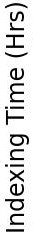
\includegraphics[width=\textwidth]{../img/oigas/CandNeighbors/legend_idx.jpg}
        \vspace{0.5cm}
    \end{subfigure}
     \centering
        \begin{subfigure}{0.28\textwidth}
        \captionsetup{justification=centering}
	\centering	
        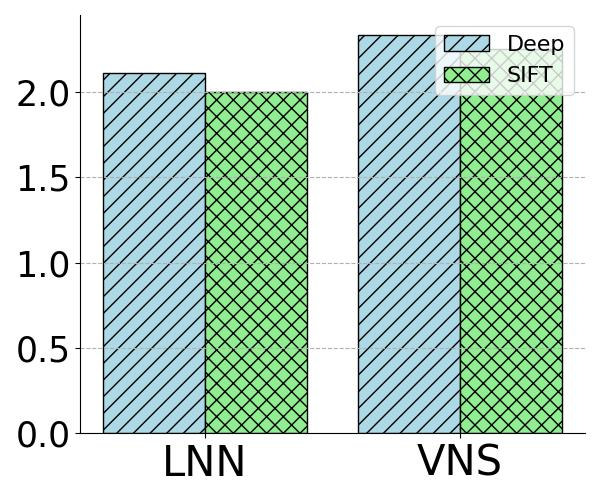
\includegraphics[width=\textwidth]{../img/oigas/CandNeighbors/25GB_Idx.jpg}
        \caption{25GB}
           \label{fig:VNvsLNN:25GB}
    \end{subfigure}    
         \begin{subfigure}{0.28\textwidth}
         \captionsetup{justification=centering}
	\centering	
        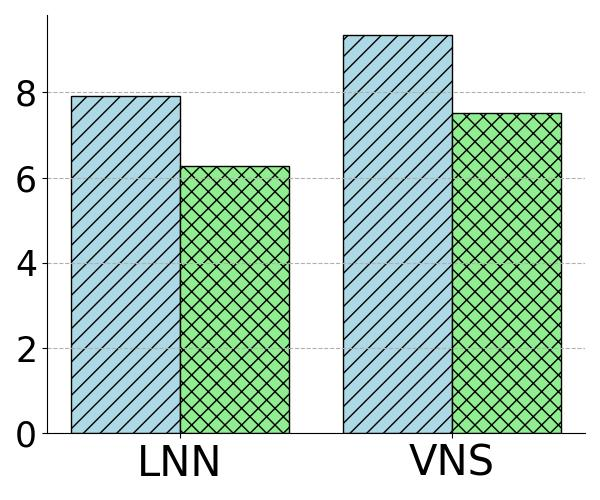
\includegraphics[width=\textwidth]{../img/oigas/CandNeighbors/100GB_Idx.jpg}
        \caption{100GB}
       \label{fig:VNvsLNN:100GB}
    \end{subfigure}    
         \begin{subfigure}{0.28\textwidth}
             \captionsetup{justification=centering}
	\centering	
        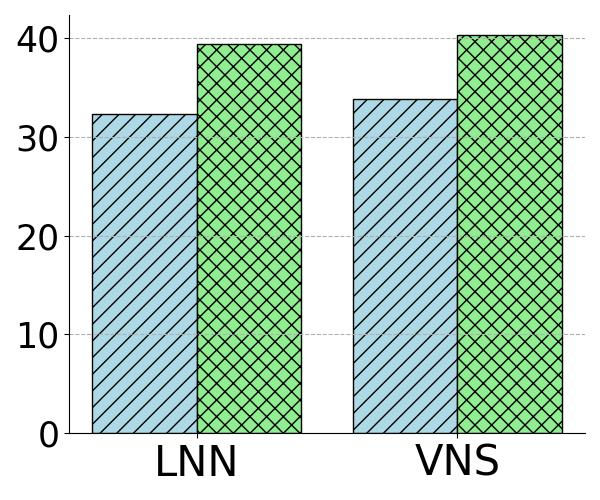
\includegraphics[width=\textwidth]{../img/oigas/CandNeighbors/1B_Idx.jpg}
        \caption{1B}
      \label{fig:VNvsLNN:1B}
    \end{subfigure}
            \caption{Indexing Time with Visited Node Set as Candidate Neighbor vs. L-NN}
            \label{fig:oigas:lnn_vs_vsn_comparison}
    \end{figure}

This figure also shows that using the visited set as candidate neighbors increases the indexing time. This is due to the necessity of managing an additional priority queue to order the visited nodes by their distance to the query. However, during the search process, we did not observe significant changes~\ref{fig:oigas:cnn}.

\begin{figure}[ht]
	\captionsetup{justification=centering}
	\centering	
        \begin{subfigure}[b]{0.2\textwidth}
            \captionsetup{justification=centering}
	\centering	
        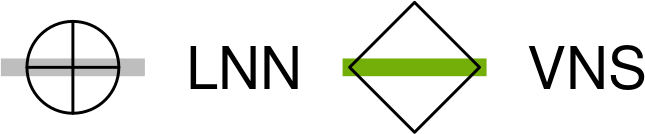
\includegraphics[width=\textwidth]{../img/oigas/CandNeighbors/search/legend.png}
    \end{subfigure}
    
    \centering
        \begin{subfigure}[b]{0.28\textwidth}
            \captionsetup{justification=centering}
	\centering	
        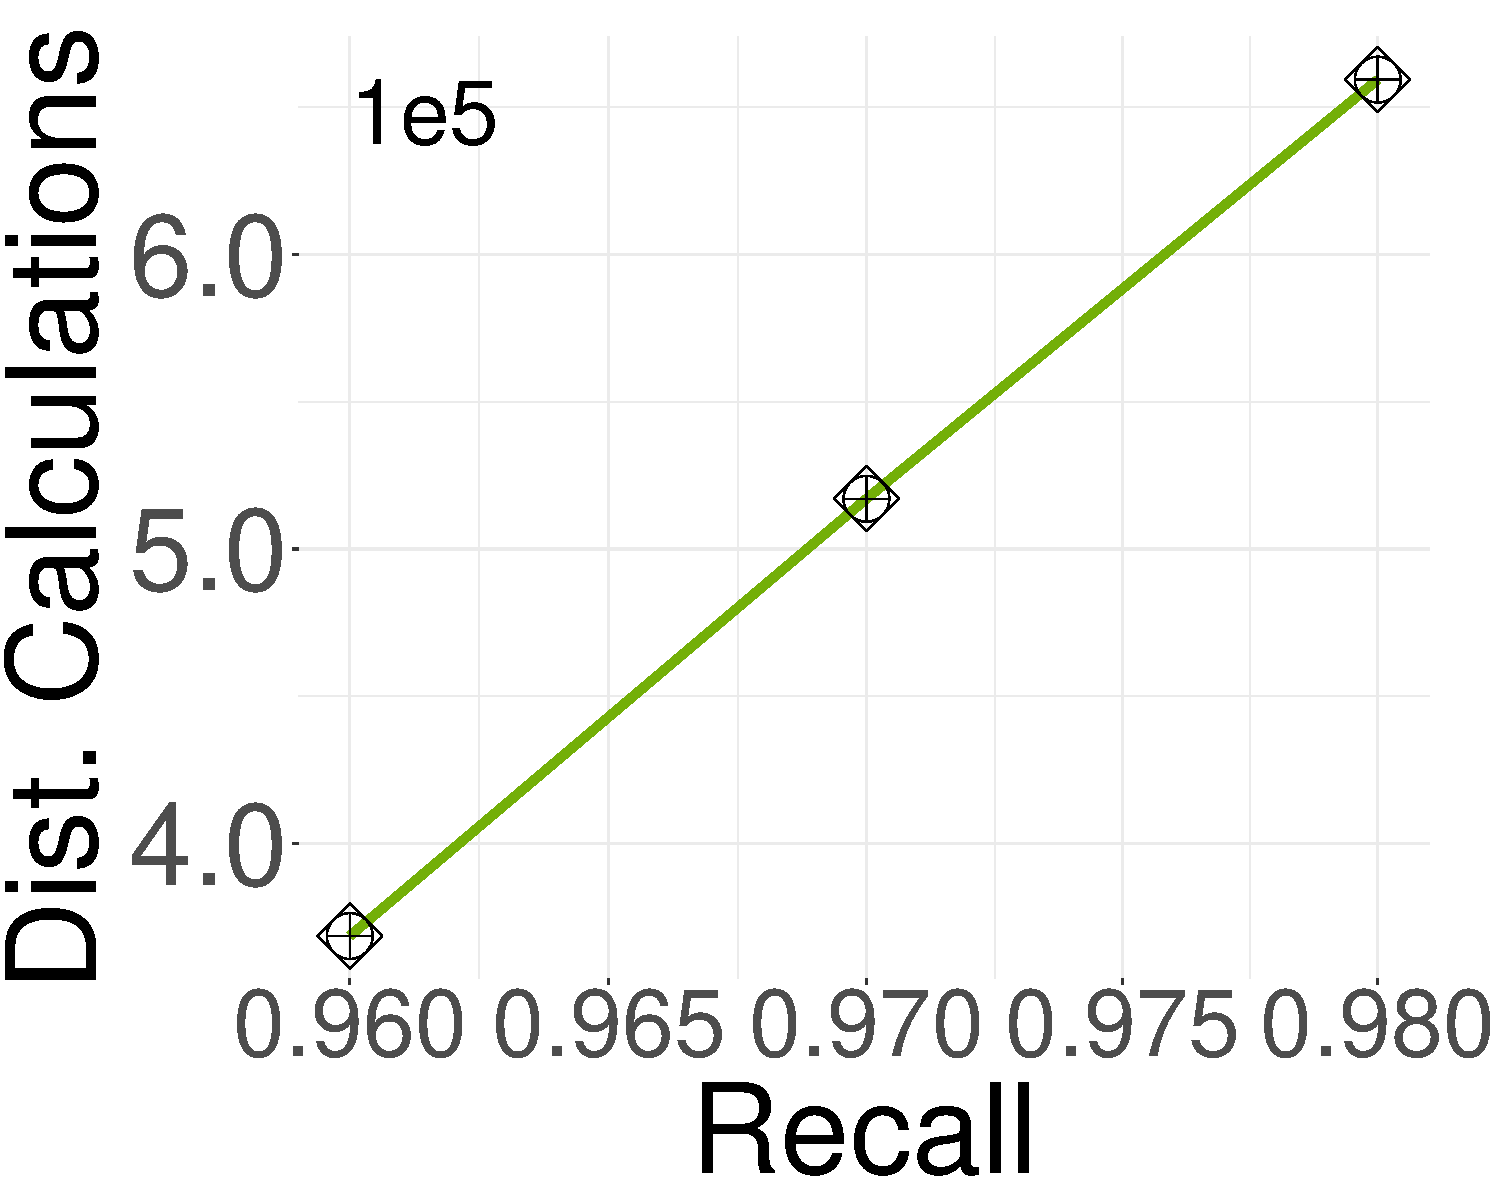
\includegraphics[width=\textwidth]{../img/oigas/CandNeighbors/search/25GB/deep_DC.pdf}
        \caption{Deep25GB}
        \label{fig:oigas:cnn:25:deep}
    \end{subfigure}
    \hspace{0.4cm}
            \begin{subfigure}[b]{0.28\textwidth}
                \captionsetup{justification=centering}
	\centering	
                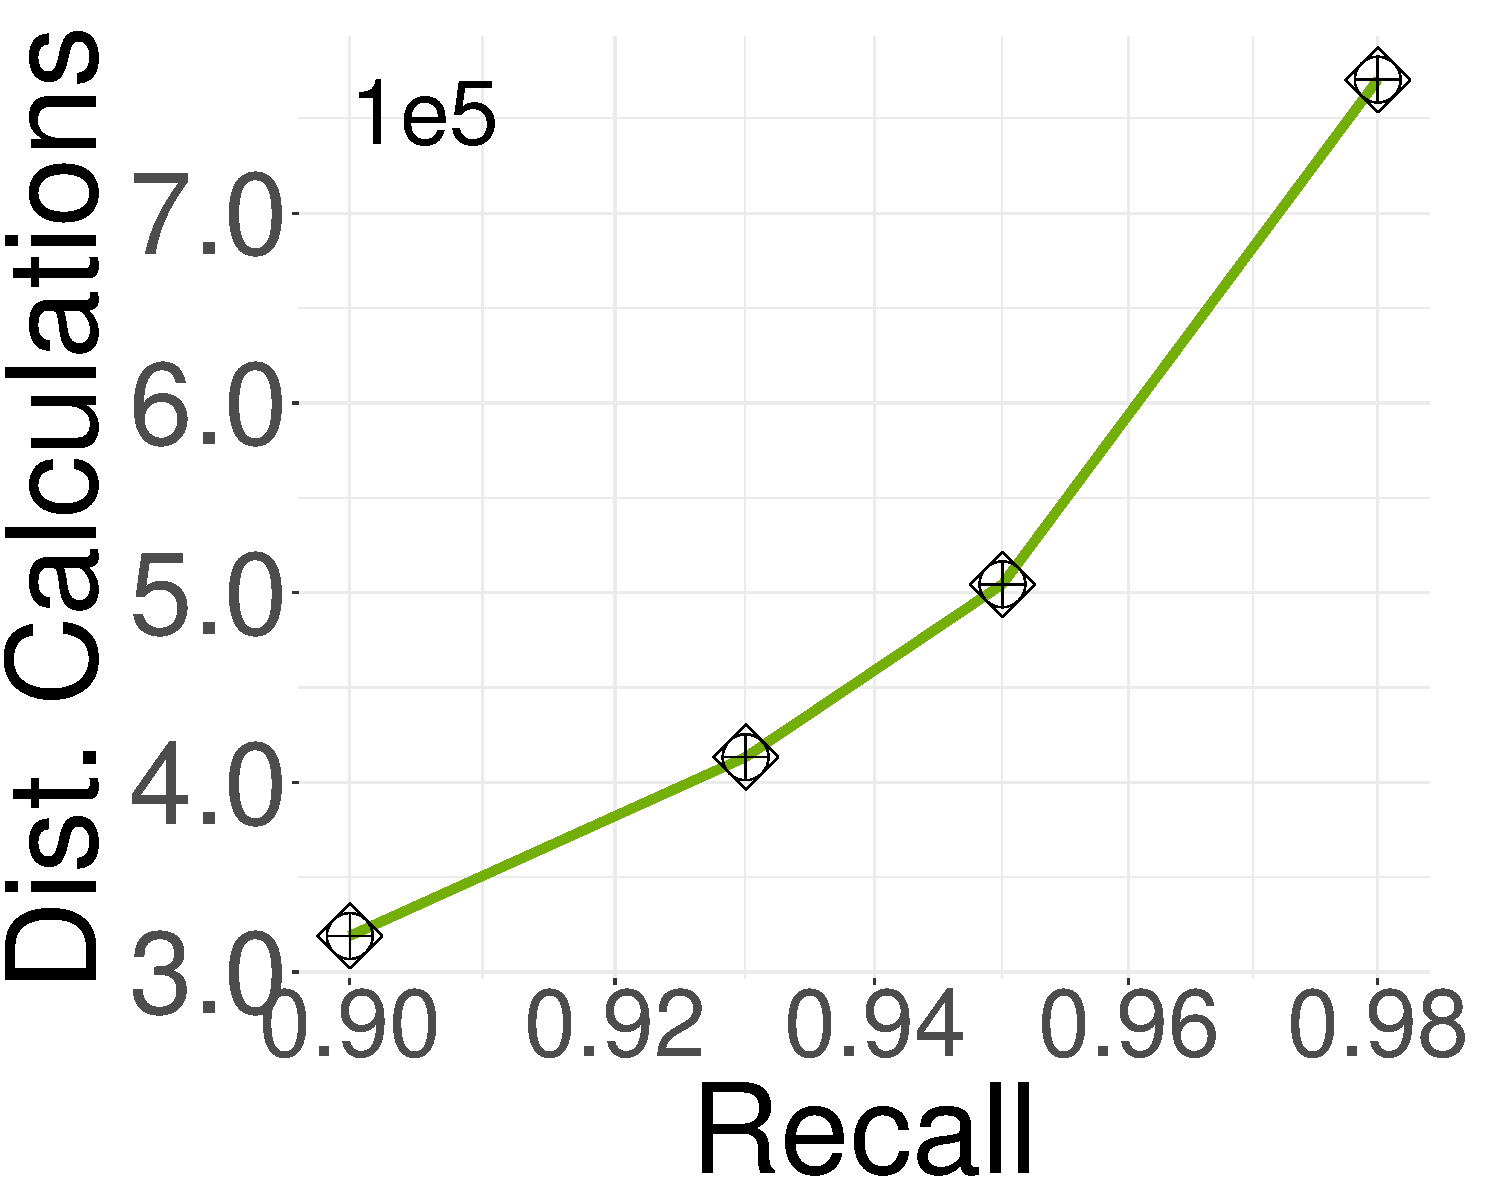
\includegraphics[width=\textwidth]{../img/oigas/CandNeighbors/search/100GB/deep_DC.pdf}
                \caption{Deep100GB}
        \label{fig:oigas:cnn:100:deep}
    \end{subfigure}
    \hspace{0.4cm}
             \begin{subfigure}[b]{0.28\textwidth}
                 \captionsetup{justification=centering}
	\centering	
                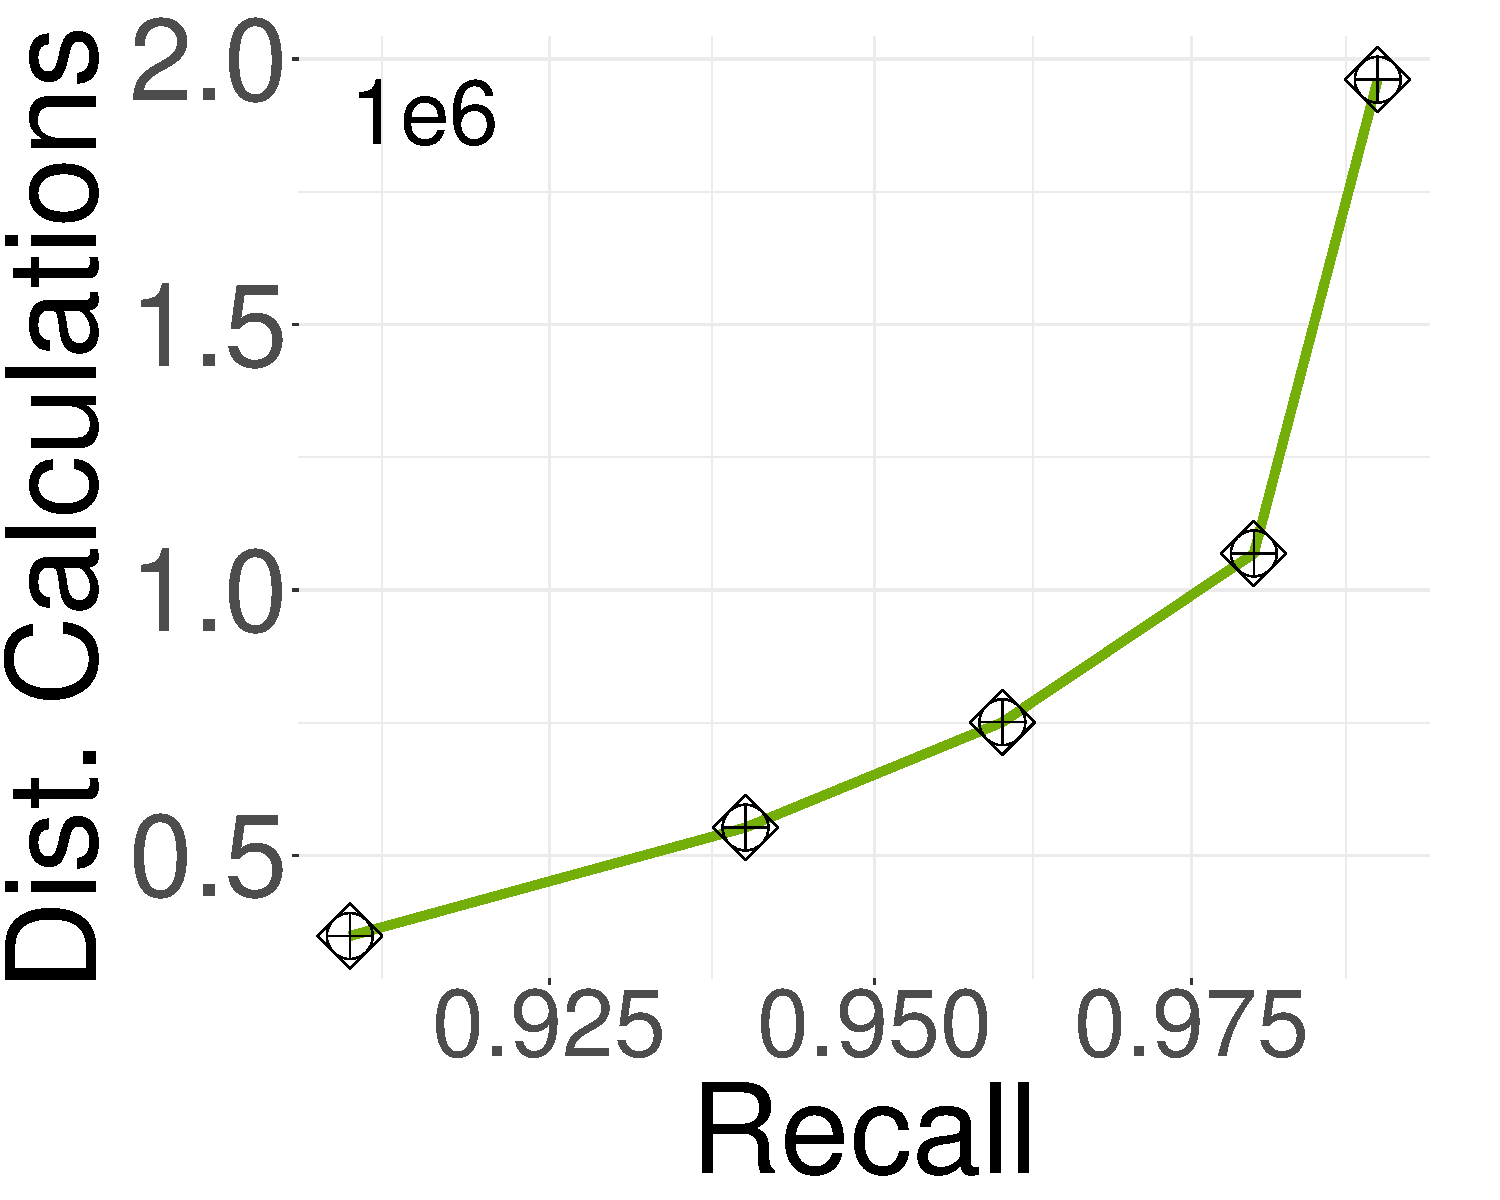
\includegraphics[width=\textwidth]{../img/oigas/CandNeighbors/search/1B/deep_DC.pdf}
        \caption{Deep1B}
        \label{fig:oigas:cnn:1B:deep}
    \end{subfigure}

          \begin{subfigure}[b]{0.28\textwidth}
              \captionsetup{justification=centering}
	\centering	
           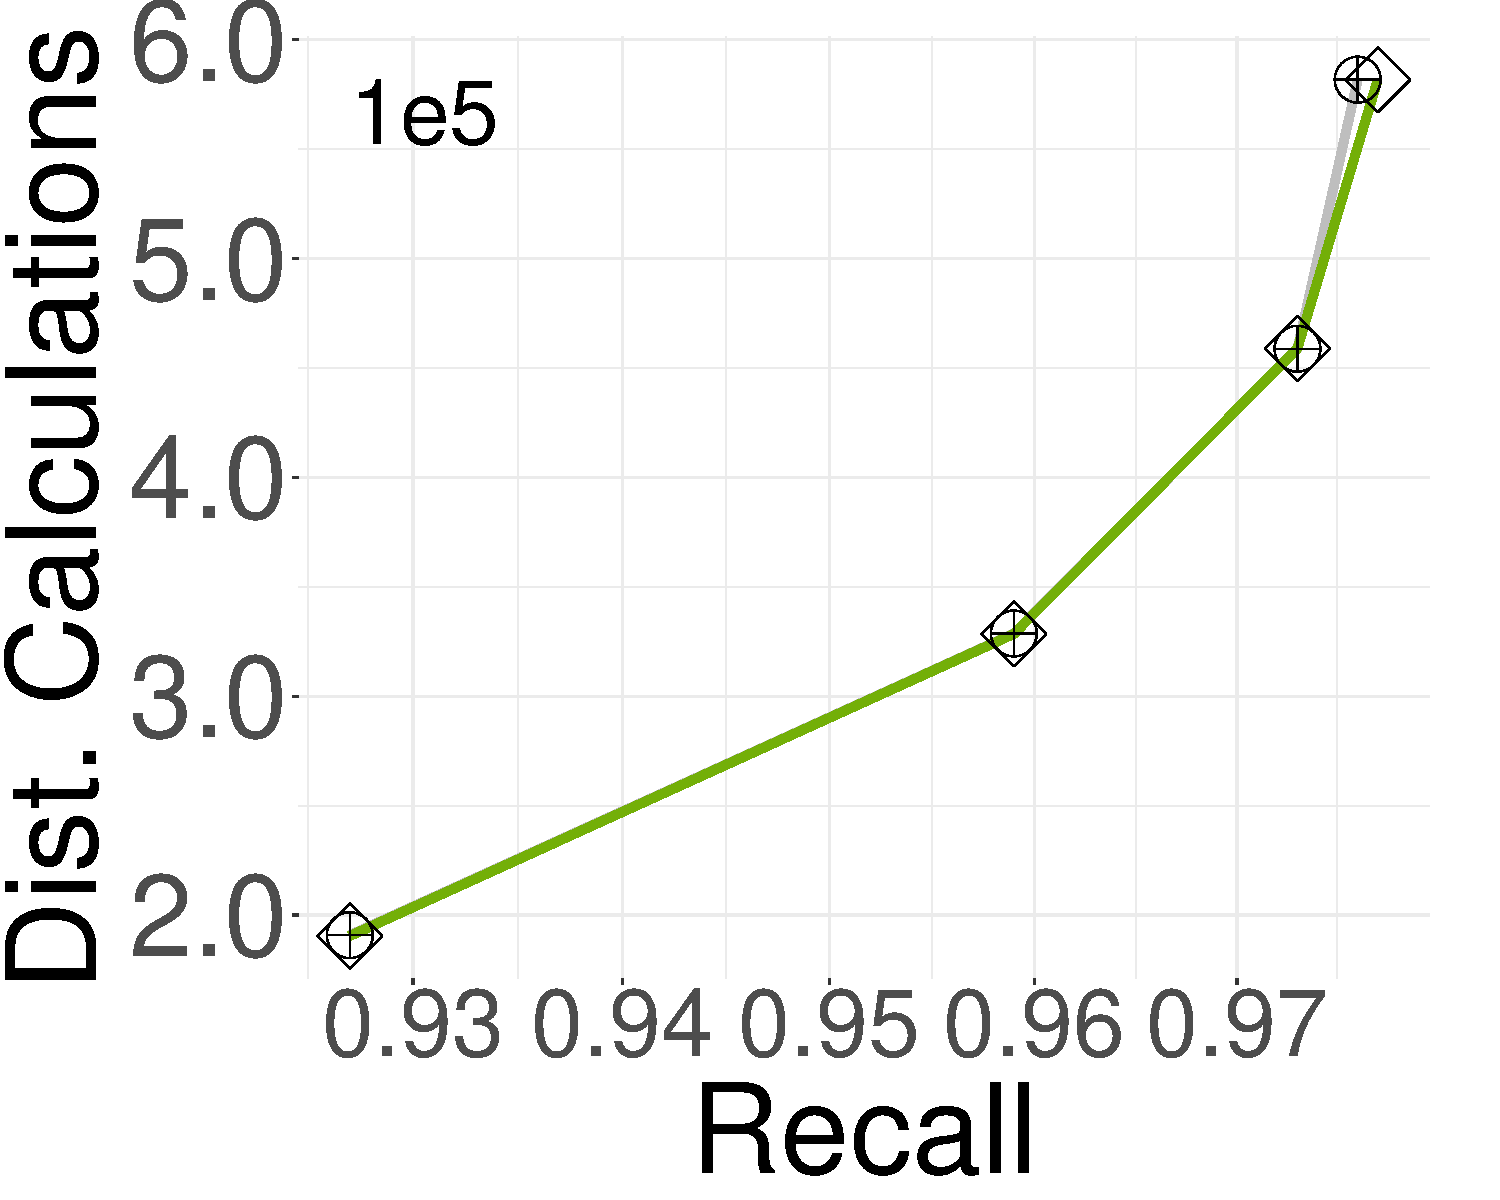
\includegraphics[width=\textwidth]{../img/oigas/CandNeighbors/search/25GB/sift_DC.pdf}
        \caption{Sift25GB}
        \label{fig:oigas:cnn:25:sift}
    \end{subfigure}
    \hspace{0.4cm}
            \begin{subfigure}[b]{0.28\textwidth}
                \captionsetup{justification=centering}
	\centering	
           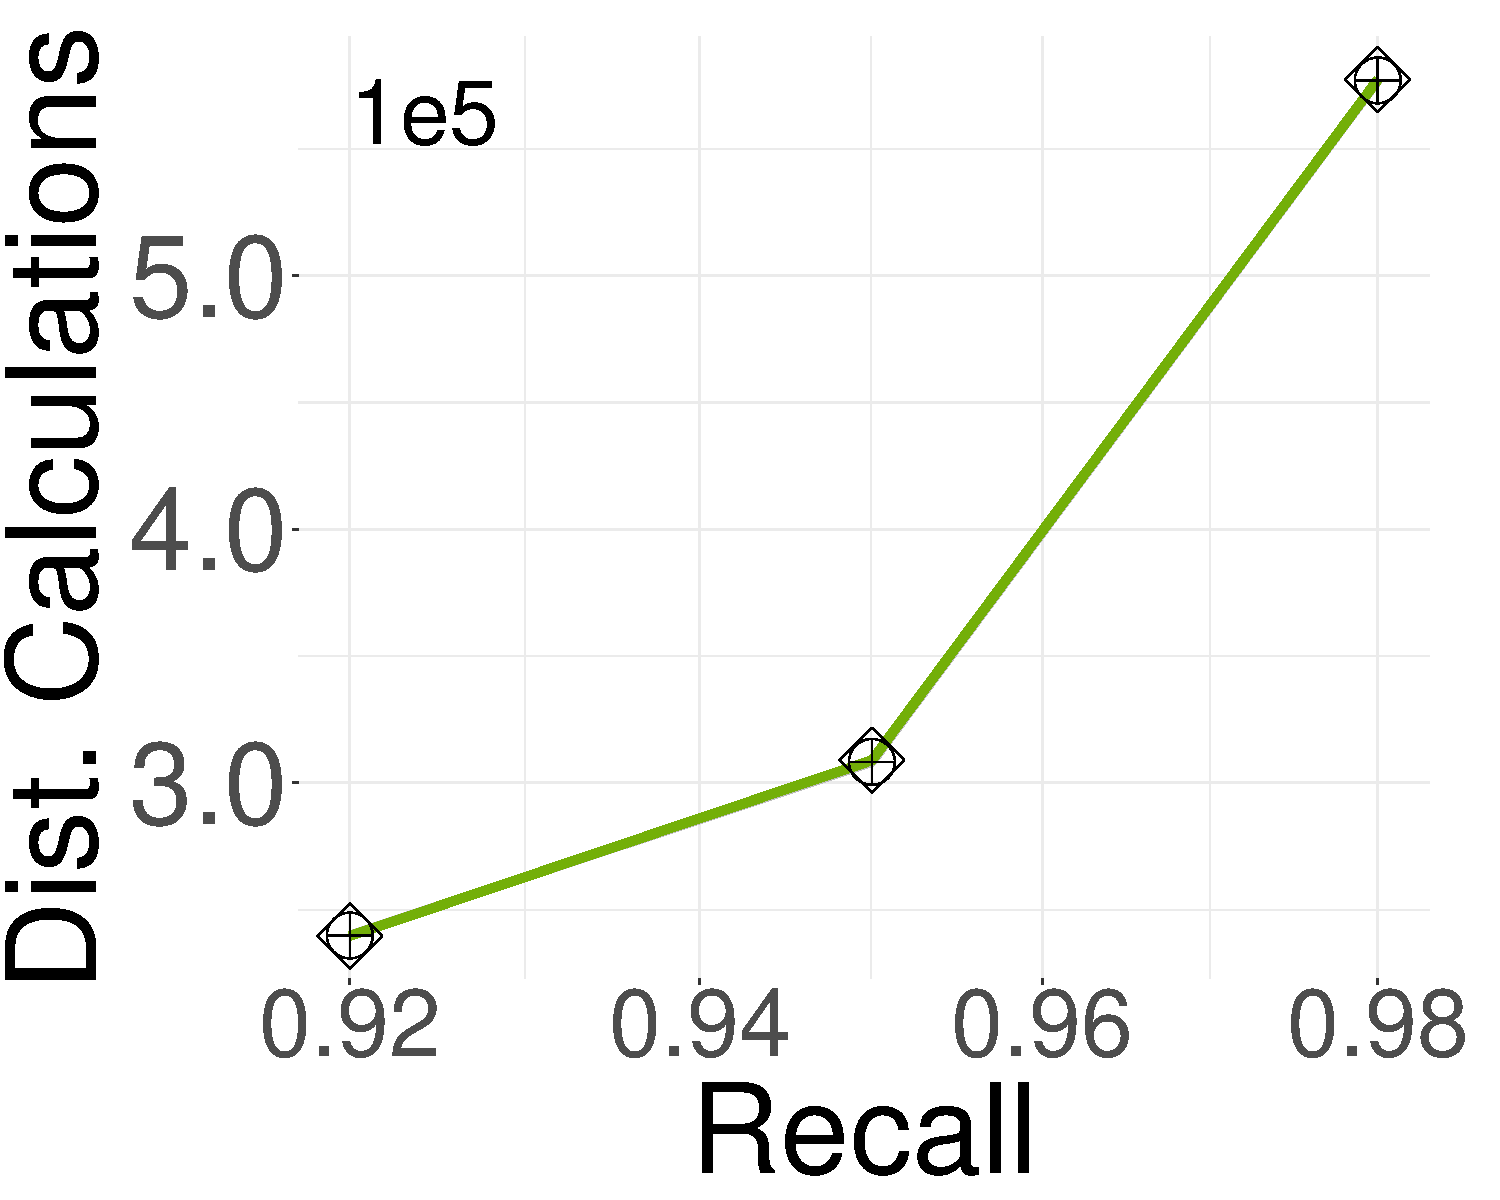
\includegraphics[width=\textwidth]{../img/oigas/CandNeighbors/search/100GB/sift_DC.pdf}
                \caption{Sift100GB}
        \label{fig:oigas:cnn:100:sift}
    \end{subfigure}
    \hspace{0.4cm}
             \begin{subfigure}[b]{0.28\textwidth}
                 \captionsetup{justification=centering}
	\centering	
           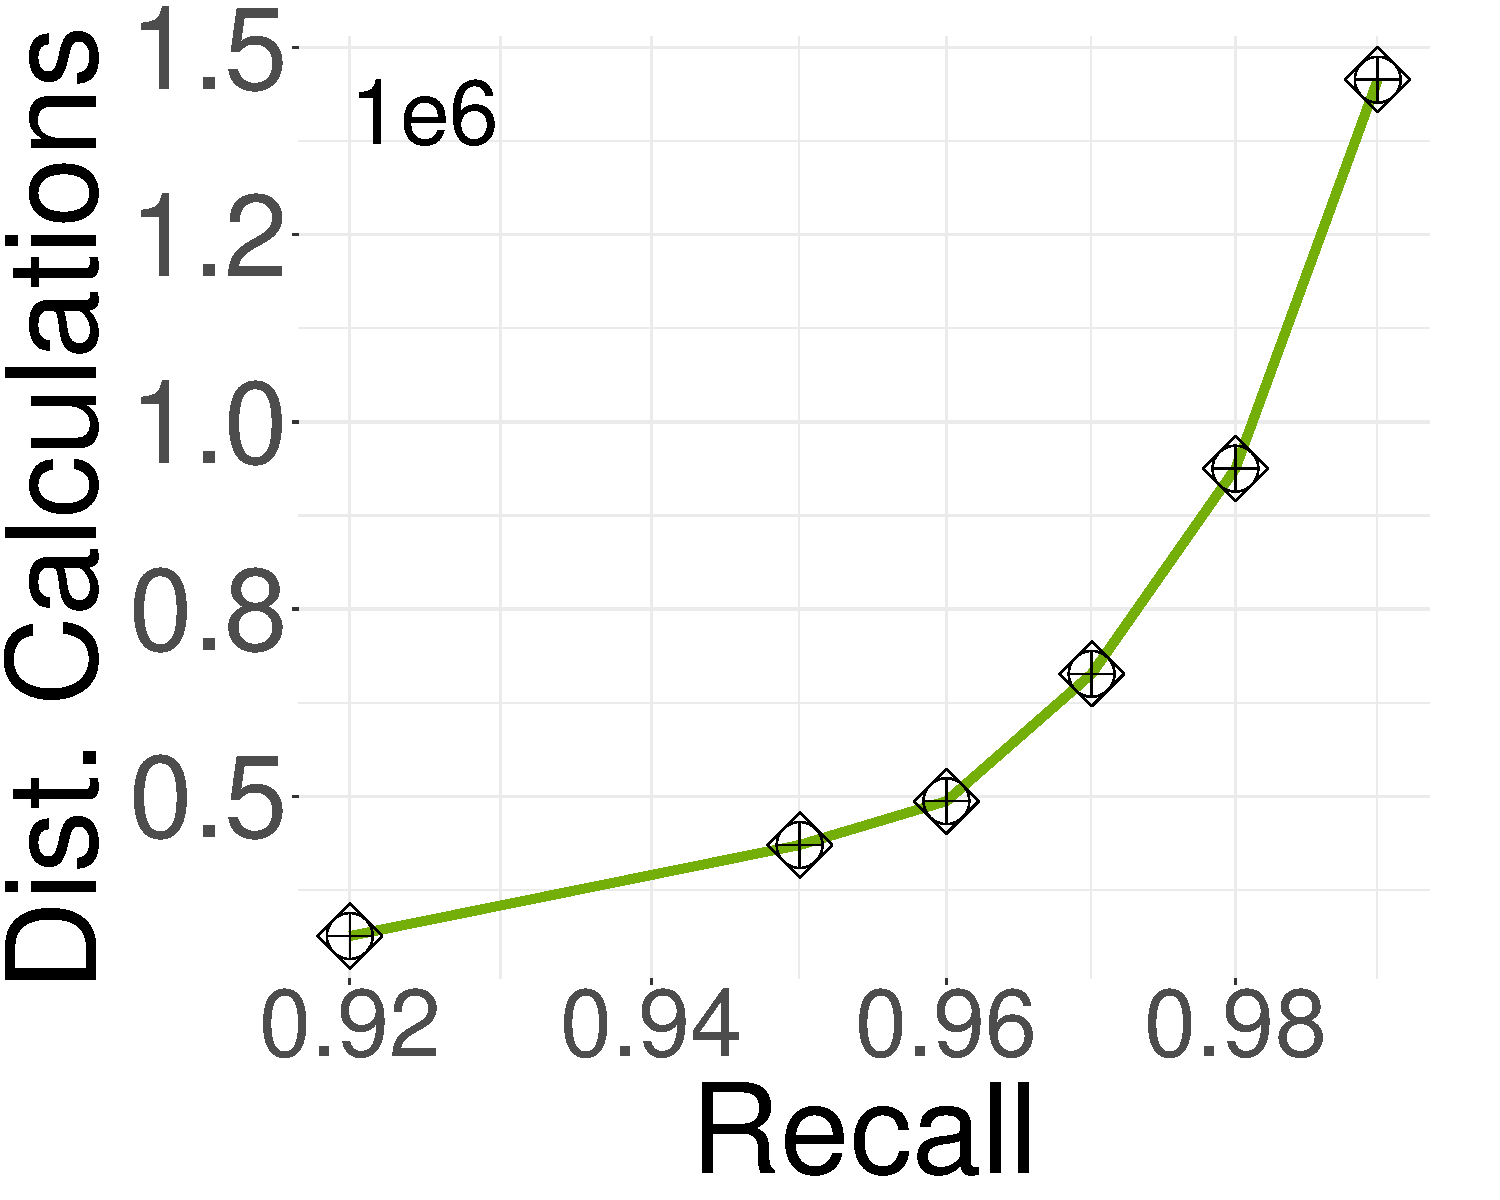
\includegraphics[width=\textwidth]{../img/oigas/CandNeighbors/search/1B/sift_DC.pdf}
        \caption{Sift1B}
        \label{fig:oigas:cnn:1B:sift}
    \end{subfigure}
    \caption{Search performance comparison of LNN vs VNS on Deep and Sift datasets}
    \label{fig:oigas:cnn}
\end{figure}

Thus, we eliminate this approach from our list, as it did not show a significant improvement to the II-based graph.

% \subsection{Ensuring Connectivity through DFS}

% A second optimization to improve the connectivity of the graph is proposed by NSG~\cite{nsg} and SSG~\cite{nssg}, which involves applying depth-first search (DFS) from random nodes to verify if there are any unreachable nodes and adding edges to connect them. This approach, however, has not been evaluated, and its impact remains unconfirmed.

% We evaluated the connectivity process of Depth-First Search (DFS) as applied by NSG and SSG after graph construction. The performance of the II-based graph with DFS connectivity checking showed no improvement in search performance, similar to the use of the visited node set discussed in the previous subsection.

\subsection{Beam Search with Single Priority Queue vs.\ Two Priority Queues}

We compared the beam search implementation of HNSW, which utilizes double priority queues, with the single priority queue beam search implementation used by other methods. HNSW uses two priority queues: the first for expansion during search, keeping track of promising yet-to-visit nodes, and the second to maintain the $L$ approximate nearest neighbors. In contrast, approaches such as Vamana and NSG use a common implementation of beam search with a single priority queue for both expansion and maintaining approximate results.
%the traditional search approach of the II-based method, HNSW, utilizing a double priority queues during search instead of single priority queue. This implementation aligns with practices common in other graph-based methods for beam search and has been shown to accelerate the search process for HNSW, attributed to its hardware-friendly \karima{???what do you mean by hardware-friendly???} nature, resulting in up to a 2.8$\times$ performance improvement on 1B-scale datasets. 
In Figure~\ref{fig:hnswdpa:25}, we illustrate how opting for the single priority queue beam search implementation in the HNSW implementation within the HNSWLib library~\cite{url/hnsw} has significantly increased HNSW search up to 2.8$\times$ while maintaining a similar number of distance calculations across various 25GB datasets. The difference in search time becomes more pronounced as we scale and increase the number of distance calculations during search, as shown in Figure~\ref{fig:hnswnew_time_and_dc}. We also observed that the stopping criteria employed by HNSWLib during search—terminating the search when the current node's distance exceeds the L-th best-so-far (BSF) distance—may negatively impact search performance on challenging datasets, as demonstrated in Figures~\ref{fig:hnswdpa:25:25GB_Seismic_DC} and~\ref{fig:hnswdpa:25:25GB_Seismic_Time}. For fair comparison, we evaluated all graph indexing methods in all previous experiments using the same single priority queue beam search implementation. 

\begin{figure}[htbp]
	\captionsetup{justification=centering}
	\centering	
\centering
    \begin{subfigure}[b]{0.4\textwidth}
        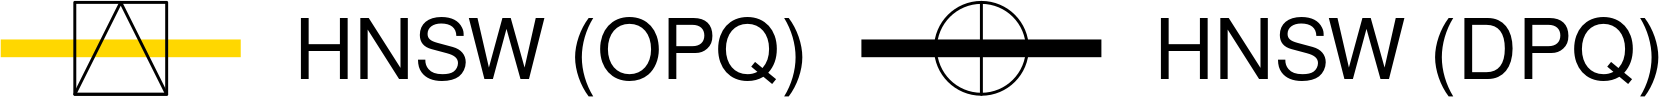
\includegraphics[width=\textwidth]{../img/oigas/PQVSPQS/legend.png}
    \end{subfigure}
    
    \centering
    \begin{subfigure}[b]{0.2325\textwidth}
        \captionsetup{justification=centering}
	\centering	
        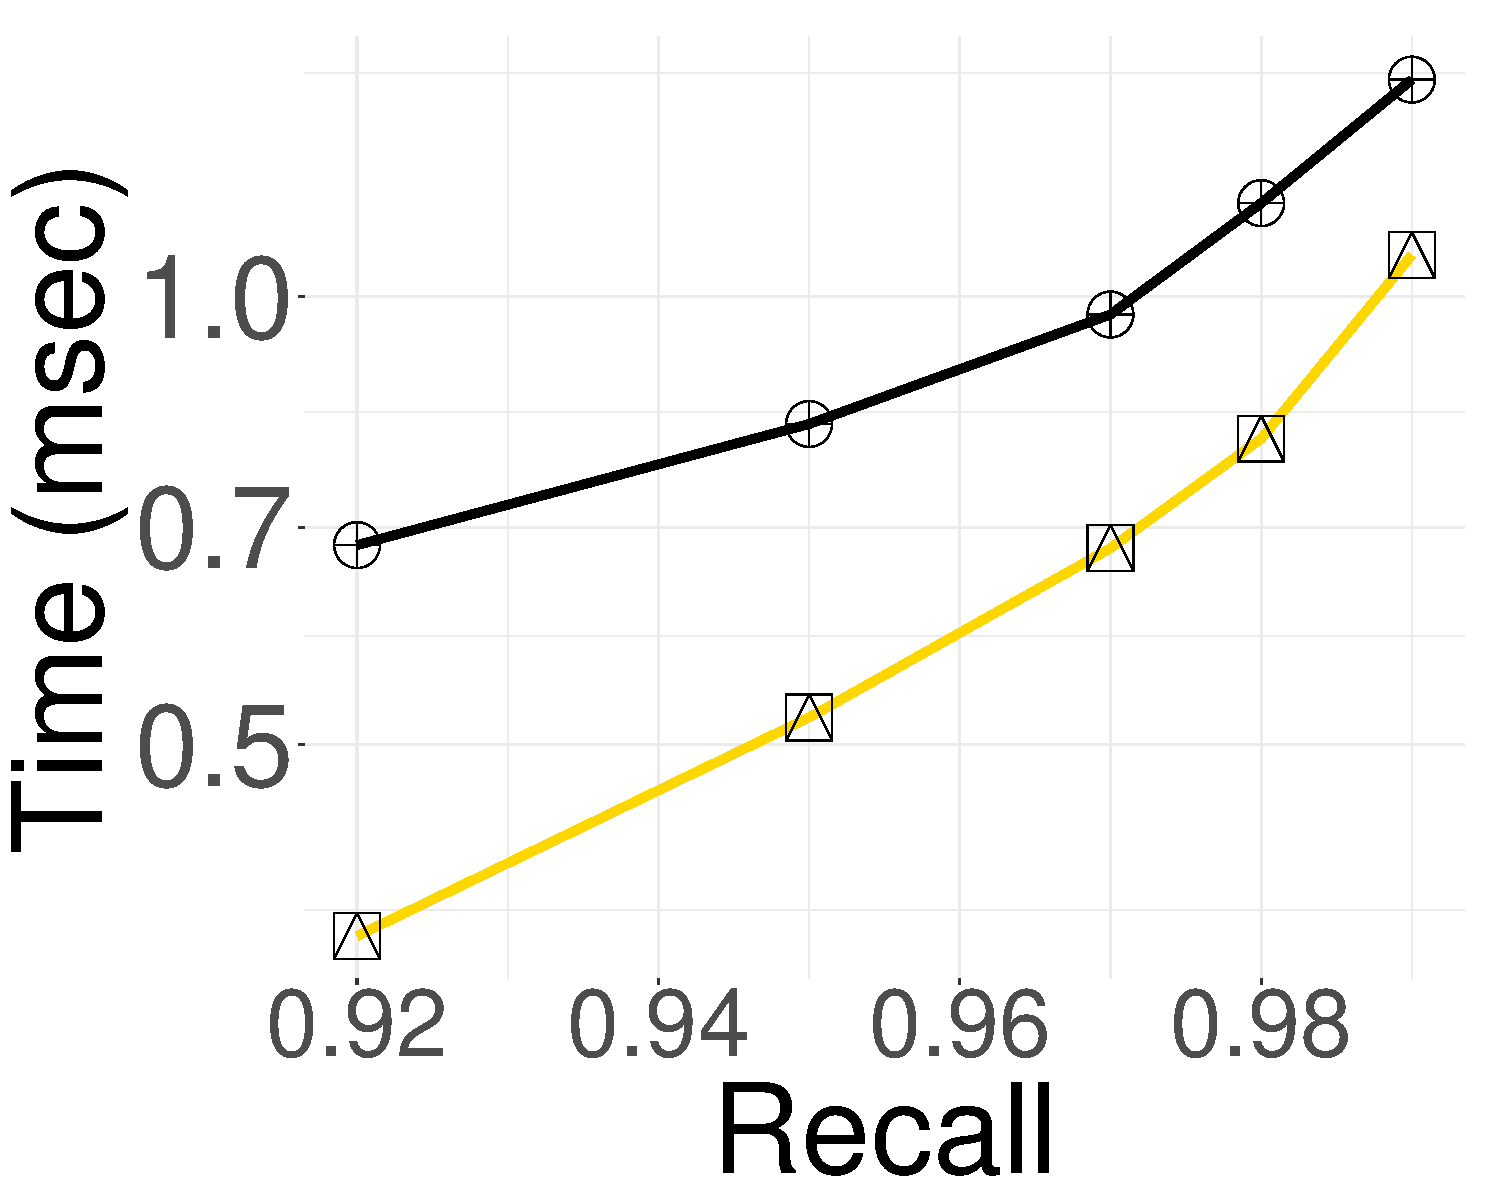
\includegraphics[width=\textwidth]{../img/oigas/PQVSPQS/25GB/deep_10_Time.pdf}
        \caption{Search Time (Deep)}
        \label{fig:hnswdpa:25:25GB_Deep_Time}
    \end{subfigure}
    \begin{subfigure}[b]{0.2325\textwidth}
        \captionsetup{justification=centering}
	\centering	
        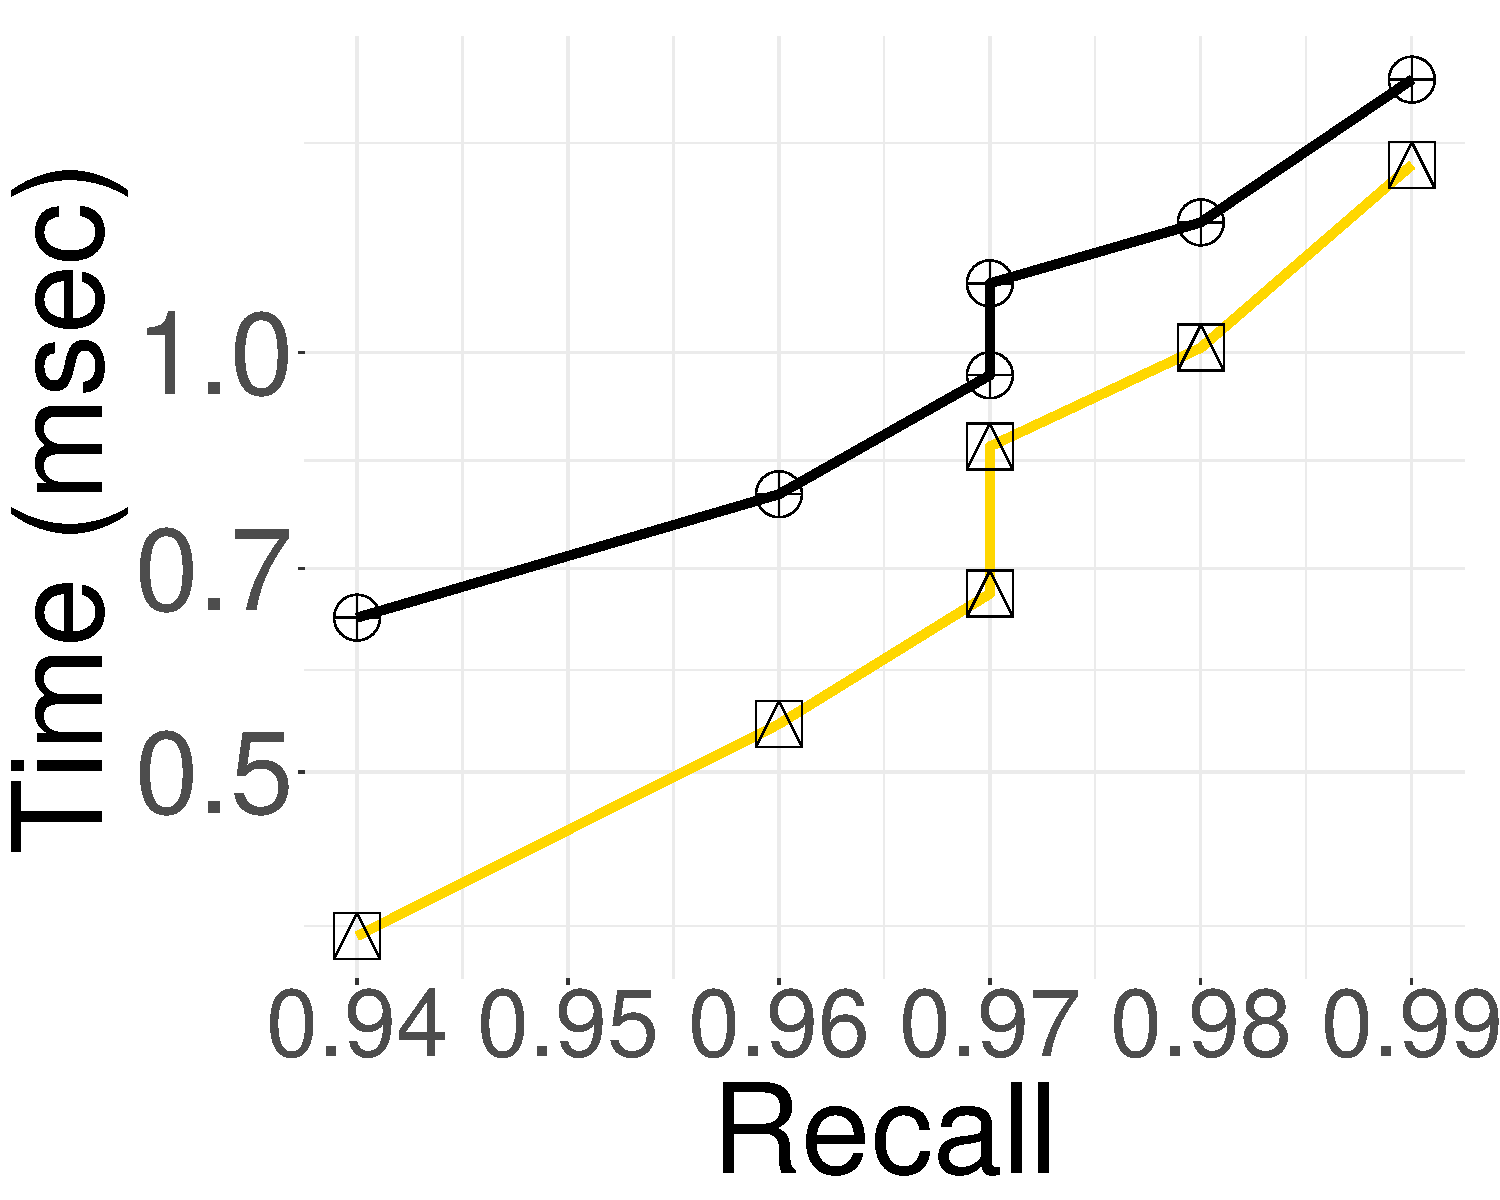
\includegraphics[width=\textwidth]{../img/oigas/PQVSPQS/25GB/sift_10_Time.pdf}
        \caption{Search Time (Sift)}
        \label{fig:hnswdpa:25:25GB_Sift_Time}
    \end{subfigure}
    \begin{subfigure}[b]{0.2325\textwidth}
        \captionsetup{justification=centering}
	\centering	
        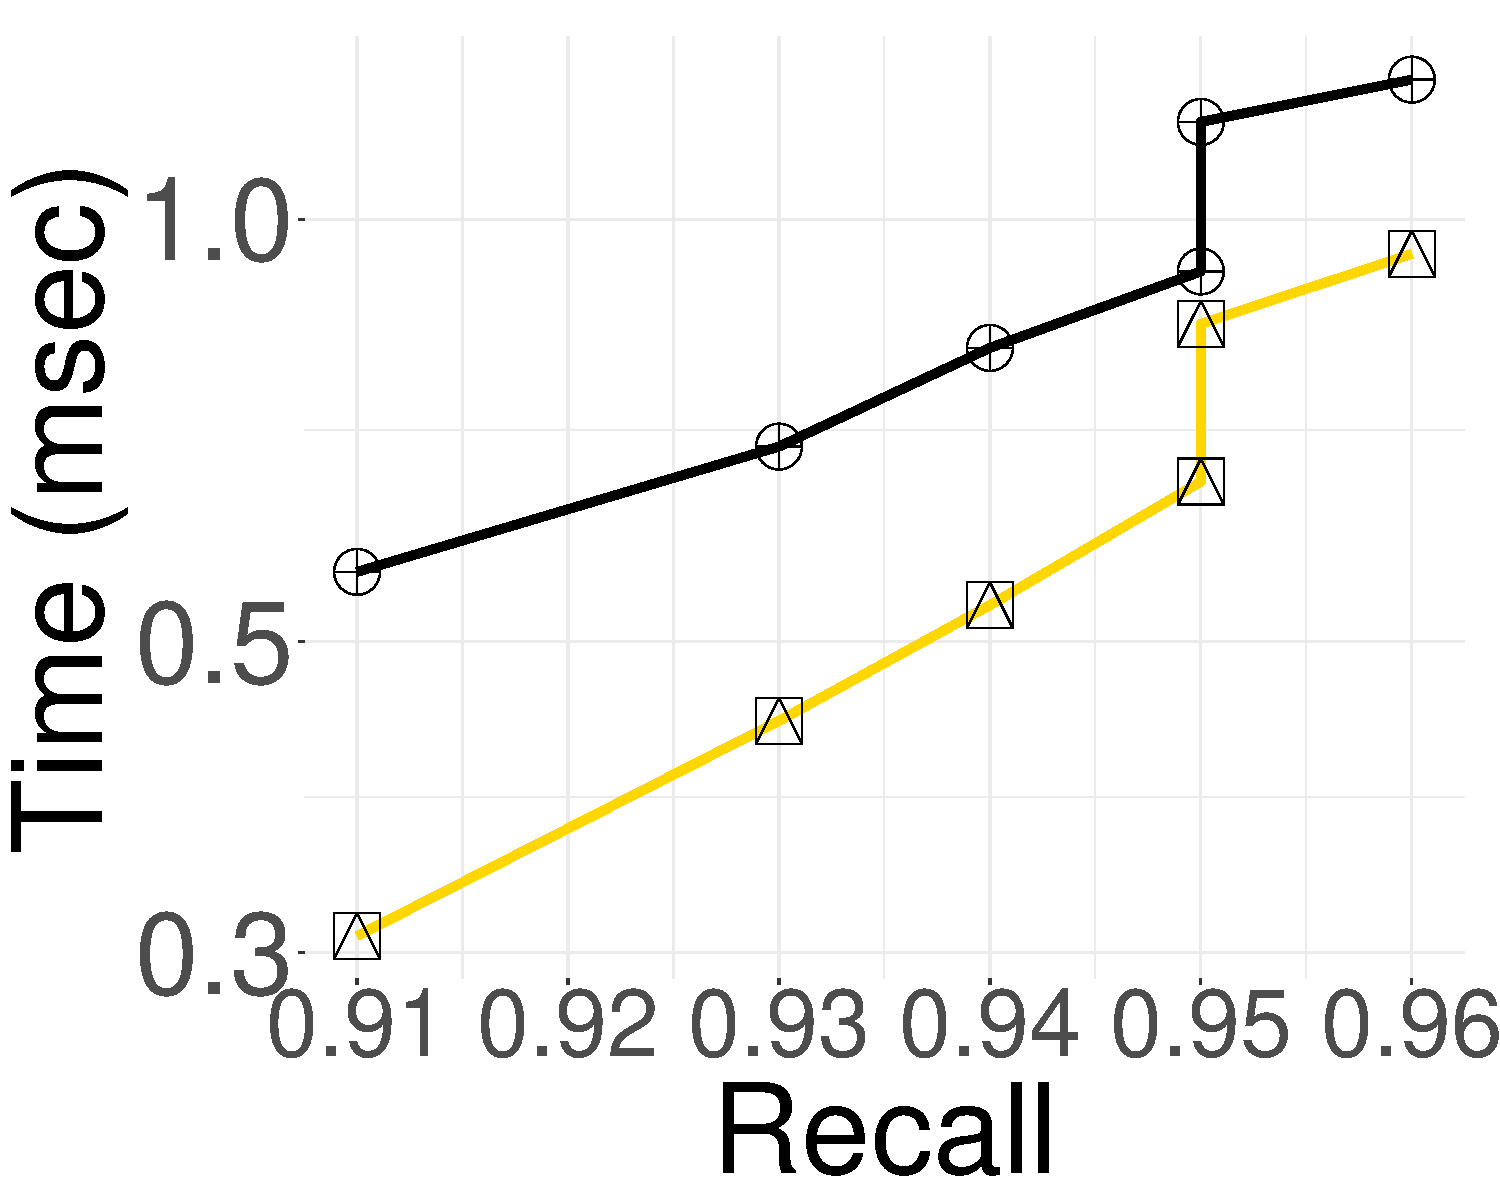
\includegraphics[width=\textwidth]{../img/oigas/PQVSPQS/25GB/sald_10_Time.pdf}
        \caption{Search Time (Sald)}
        \label{fig:hnswdpa:25:25GB_Sald_Time}
    \end{subfigure}
    \begin{subfigure}[b]{0.2325\textwidth}
        \captionsetup{justification=centering}
	\centering	
        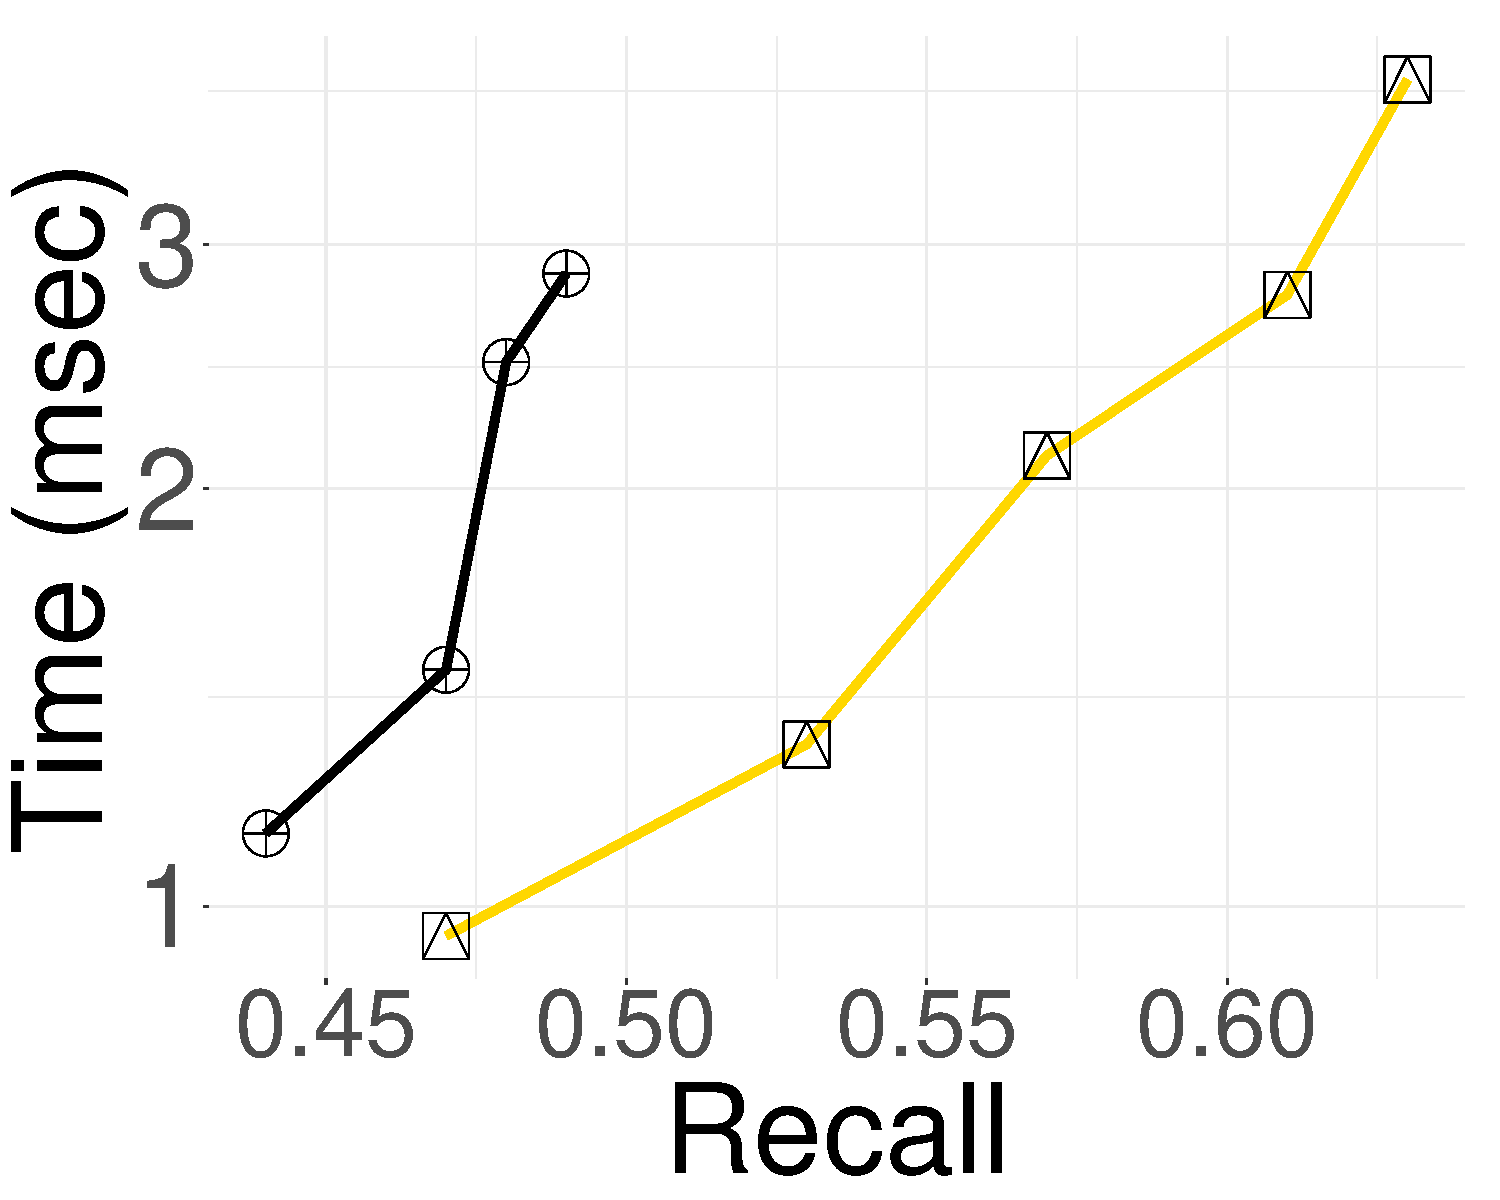
\includegraphics[width=\textwidth]{../img/oigas/PQVSPQS/25GB/seismic_10_Time.pdf}
        \caption{Search Time (Seismic)}
        \label{fig:hnswdpa:25:25GB_Seismic_Time}
    \end{subfigure}
    
    % Second row: Number of Distance Calculations
    \begin{subfigure}[b]{0.2325\textwidth}
        \captionsetup{justification=centering}
	\centering	
        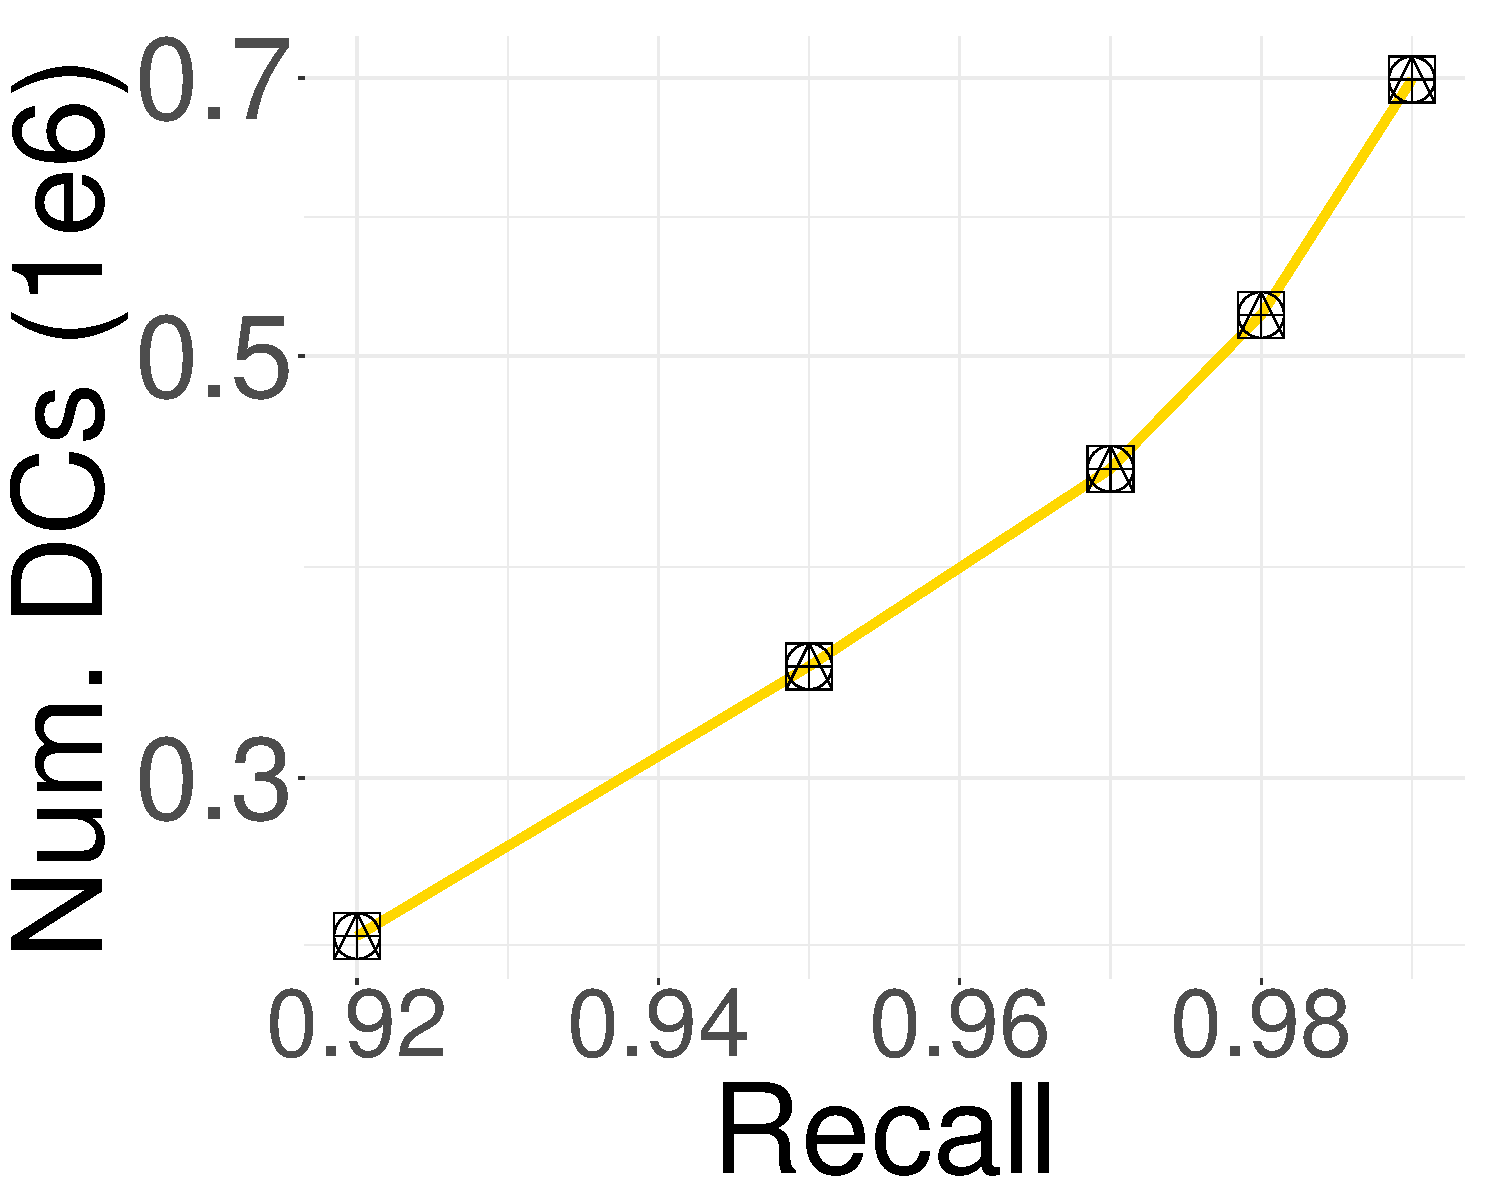
\includegraphics[width=\textwidth]{../img/oigas/PQVSPQS/25GB/deep_10_DC.pdf}
        \caption{Num. Dcs (Deep)}
        \label{fig:hnswdpa:25:25GB_Deep_DC}
    \end{subfigure}
    \begin{subfigure}[b]{0.2325\textwidth}
        \captionsetup{justification=centering}
	\centering	
        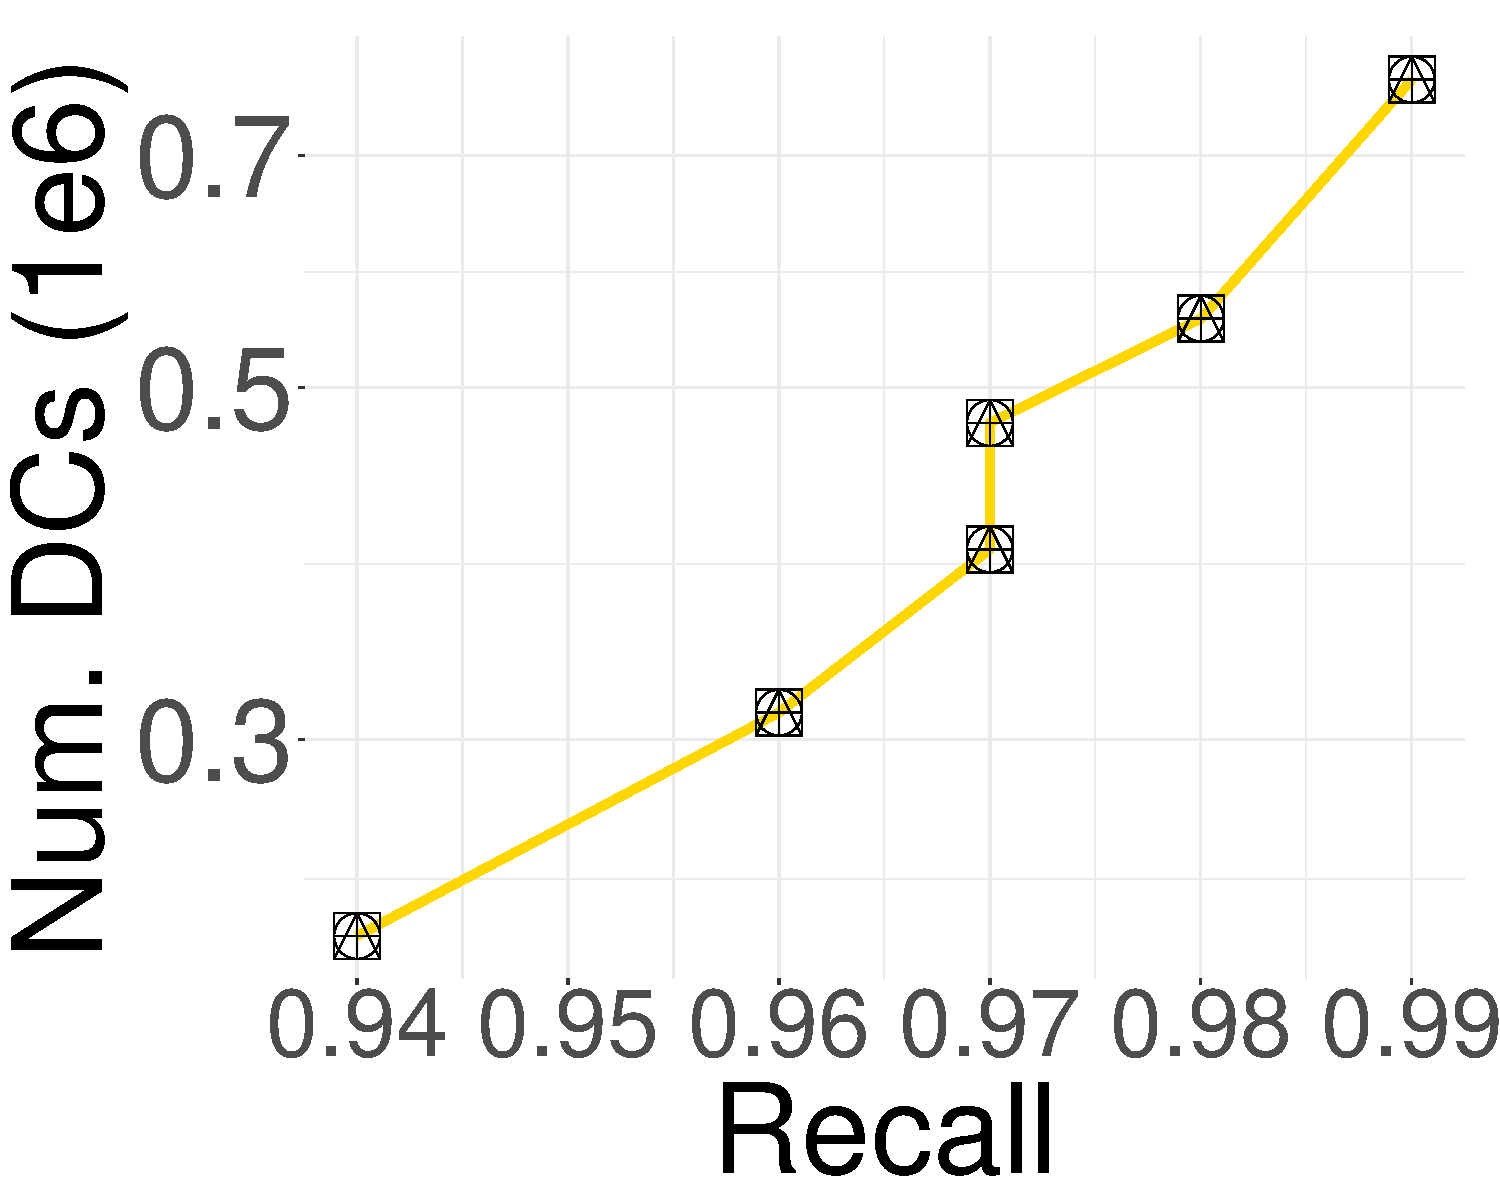
\includegraphics[width=\textwidth]{../img/oigas/PQVSPQS/25GB/sift_10_DC.pdf}
        \caption{Num. Dcs (Sift)}
        \label{fig:hnswdpa:25:25GB_Sift_DC}
    \end{subfigure}
    \begin{subfigure}[b]{0.2325\textwidth}
        \captionsetup{justification=centering}
	\centering	
        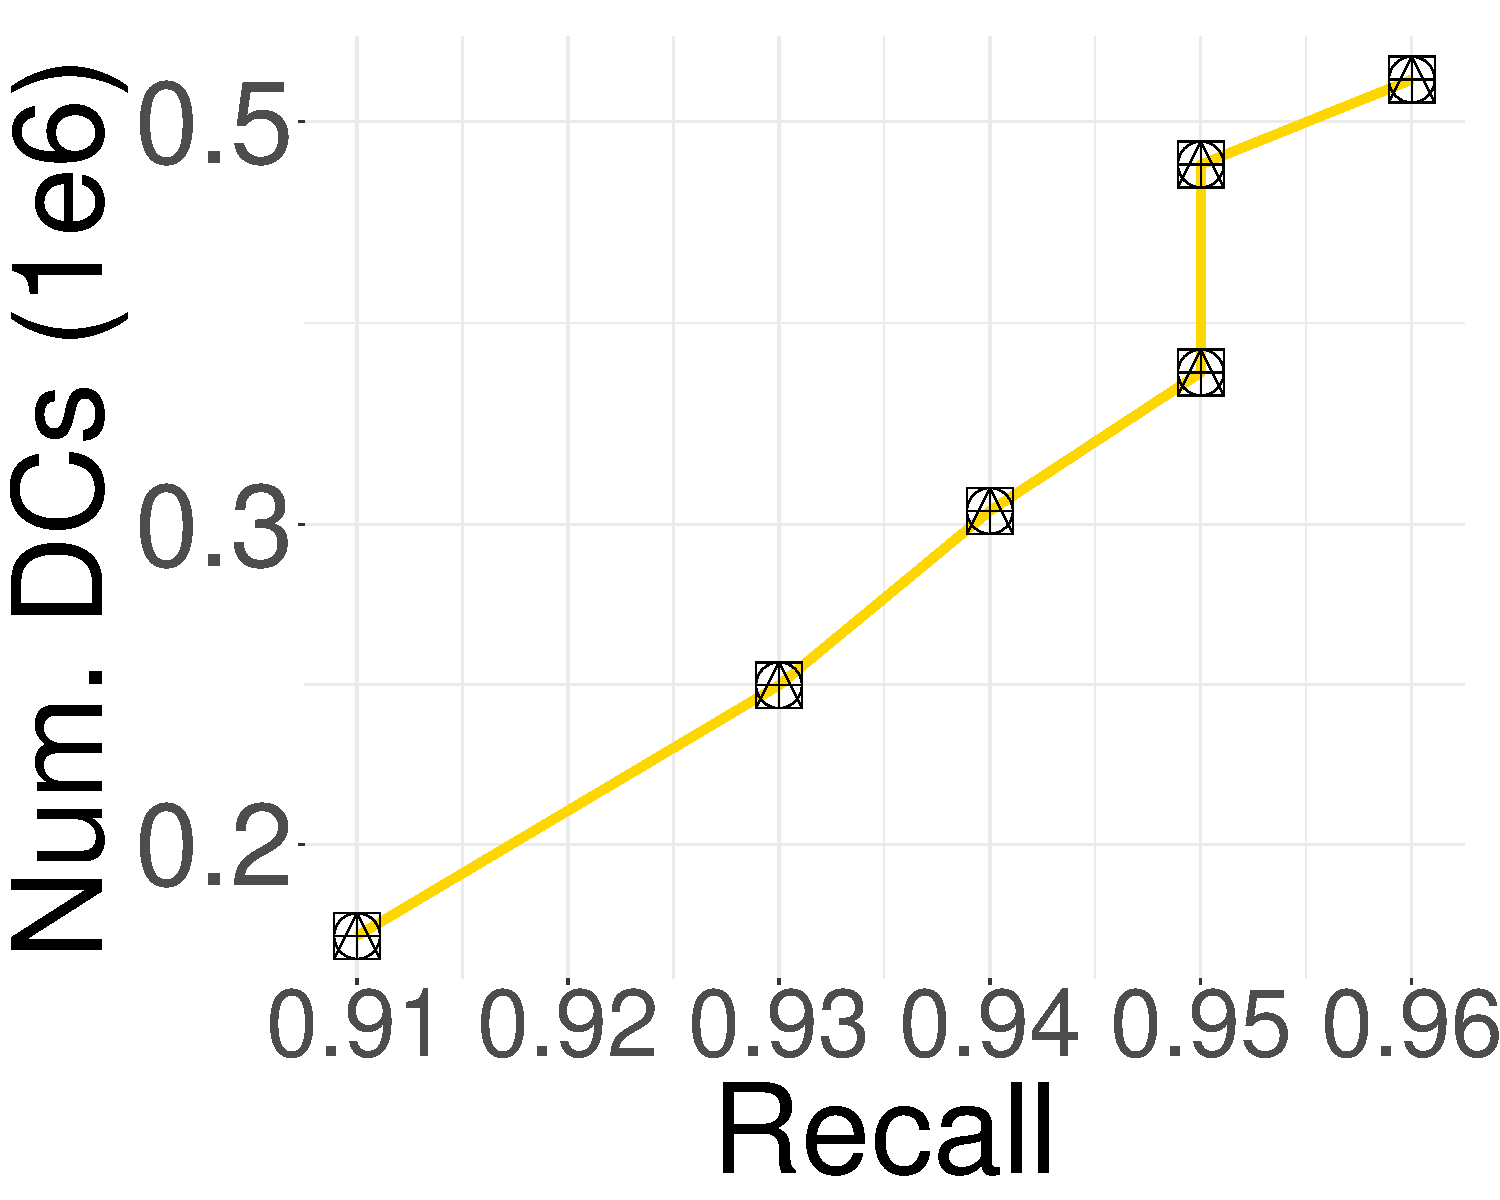
\includegraphics[width=\textwidth]{../img/oigas/PQVSPQS/25GB/sald_10_DC.pdf}
        \caption{Num. Dcs (Sald)}
        \label{fig:hnswdpa:25:25GB_Sald_DC}
    \end{subfigure}
    \begin{subfigure}[b]{0.2325\textwidth}
        \captionsetup{justification=centering}
	\centering	
        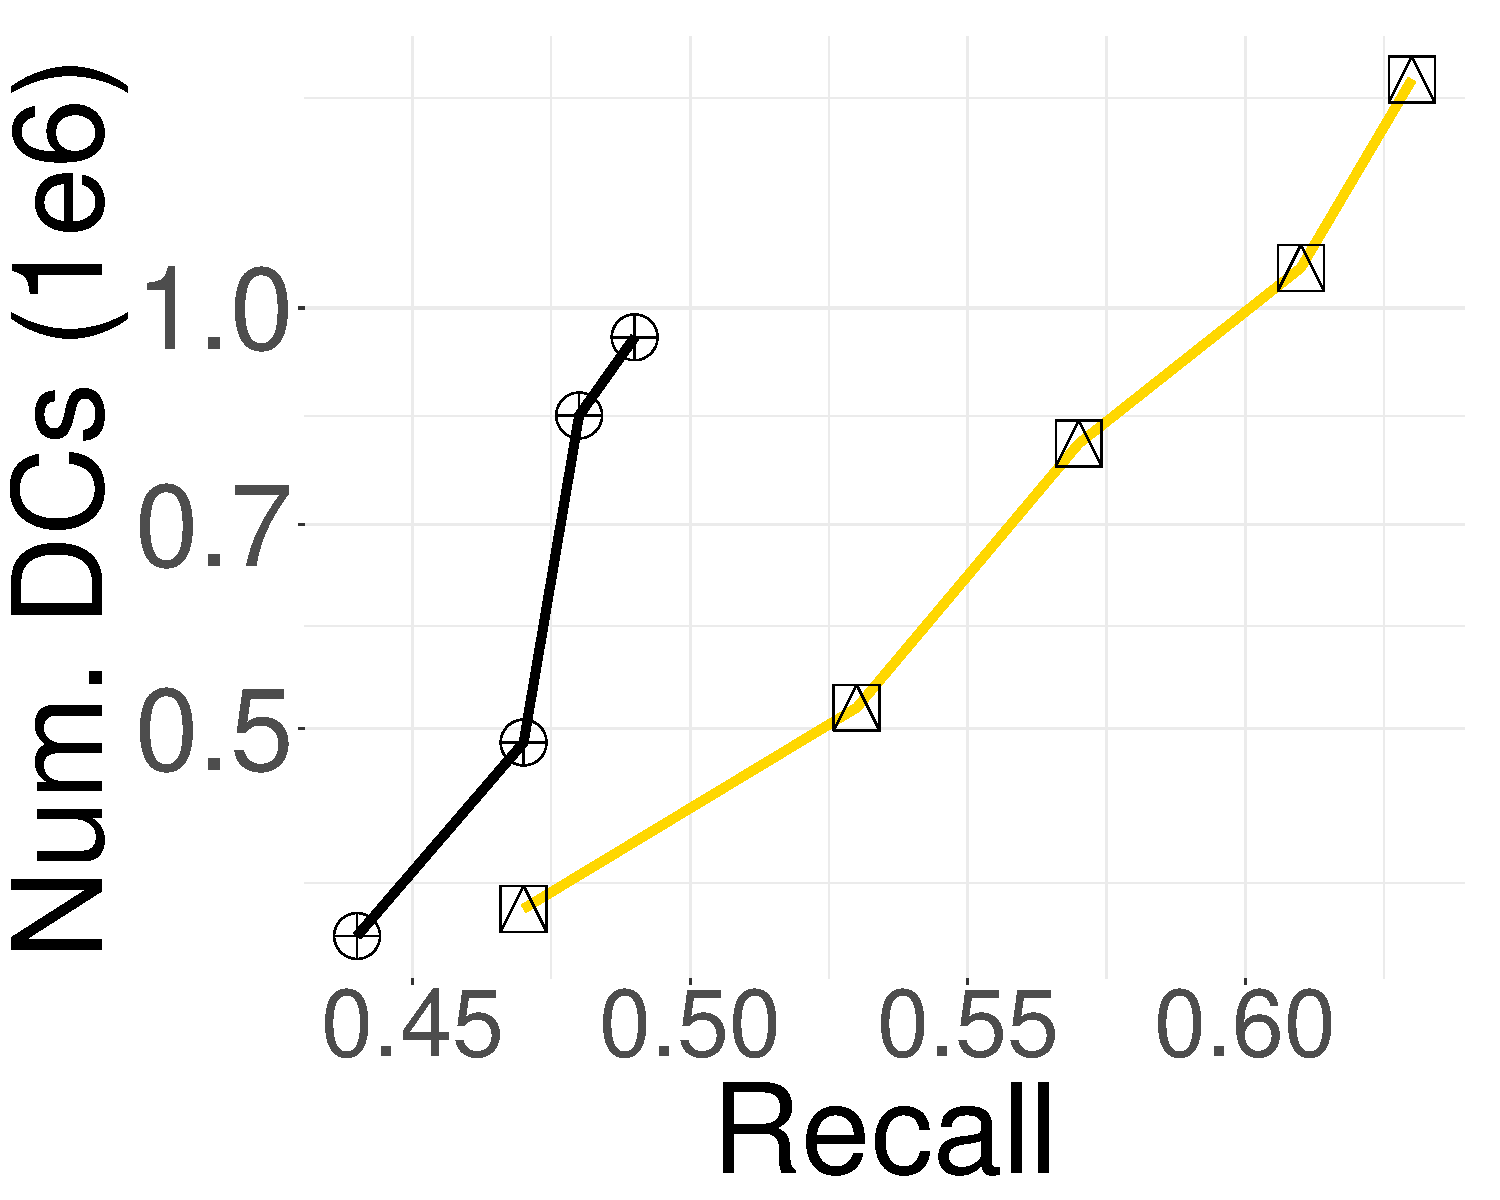
\includegraphics[width=\textwidth]{../img/oigas/PQVSPQS/25GB/seismic_10_DC.pdf}
        \caption{Num. Dcs (Seismic)}
        \label{fig:hnswdpa:25:25GB_Seismic_DC}
    \end{subfigure}
    \caption{Search Time and Number of Distance Calculations vs. Accuracy for Various Datasets at 25GB}
    \label{fig:hnswdpa:25}
\end{figure}
\begin{figure}[htbp]
	\captionsetup{justification=centering}
	\centering	
\centering
    \begin{subfigure}[b]{0.4\textwidth}
        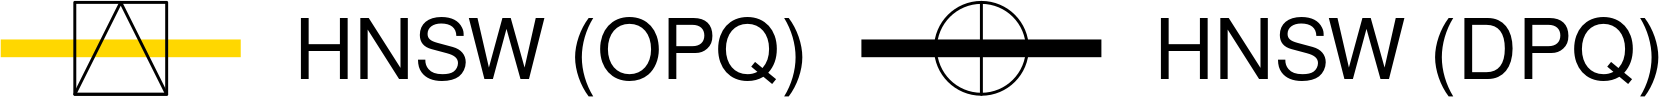
\includegraphics[width=\textwidth]{../img/oigas/PQVSPQS/legend.png}
    \end{subfigure}
    
    \centering
    \begin{subfigure}[b]{0.28\textwidth}
        \captionsetup{justification=centering}
	\centering	
        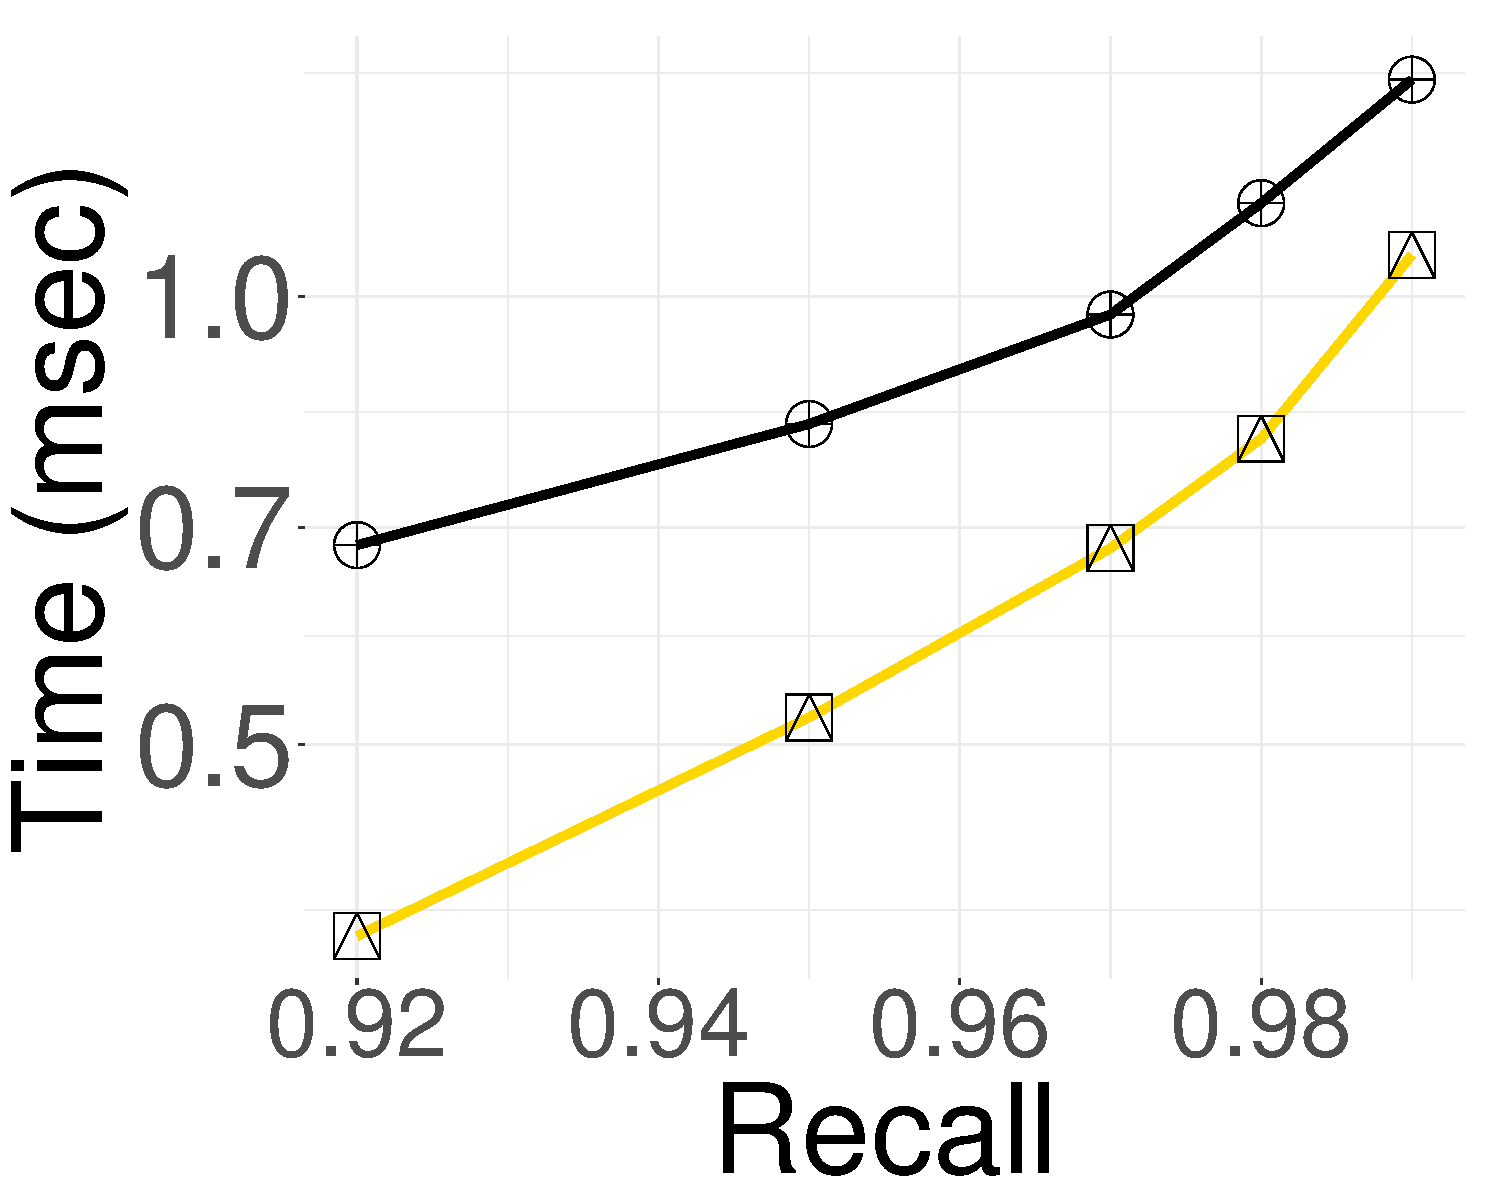
\includegraphics[width=\textwidth]{../img/oigas/PQVSPQS/25GB/deep_10_Time.pdf}
        \caption{Search Time (25GB)}
        \label{fig:SPQ:25GB_Time}
    \end{subfigure}
    \hspace{0.4cm}
    \begin{subfigure}[b]{0.28\textwidth}
        \captionsetup{justification=centering}
	\centering	
        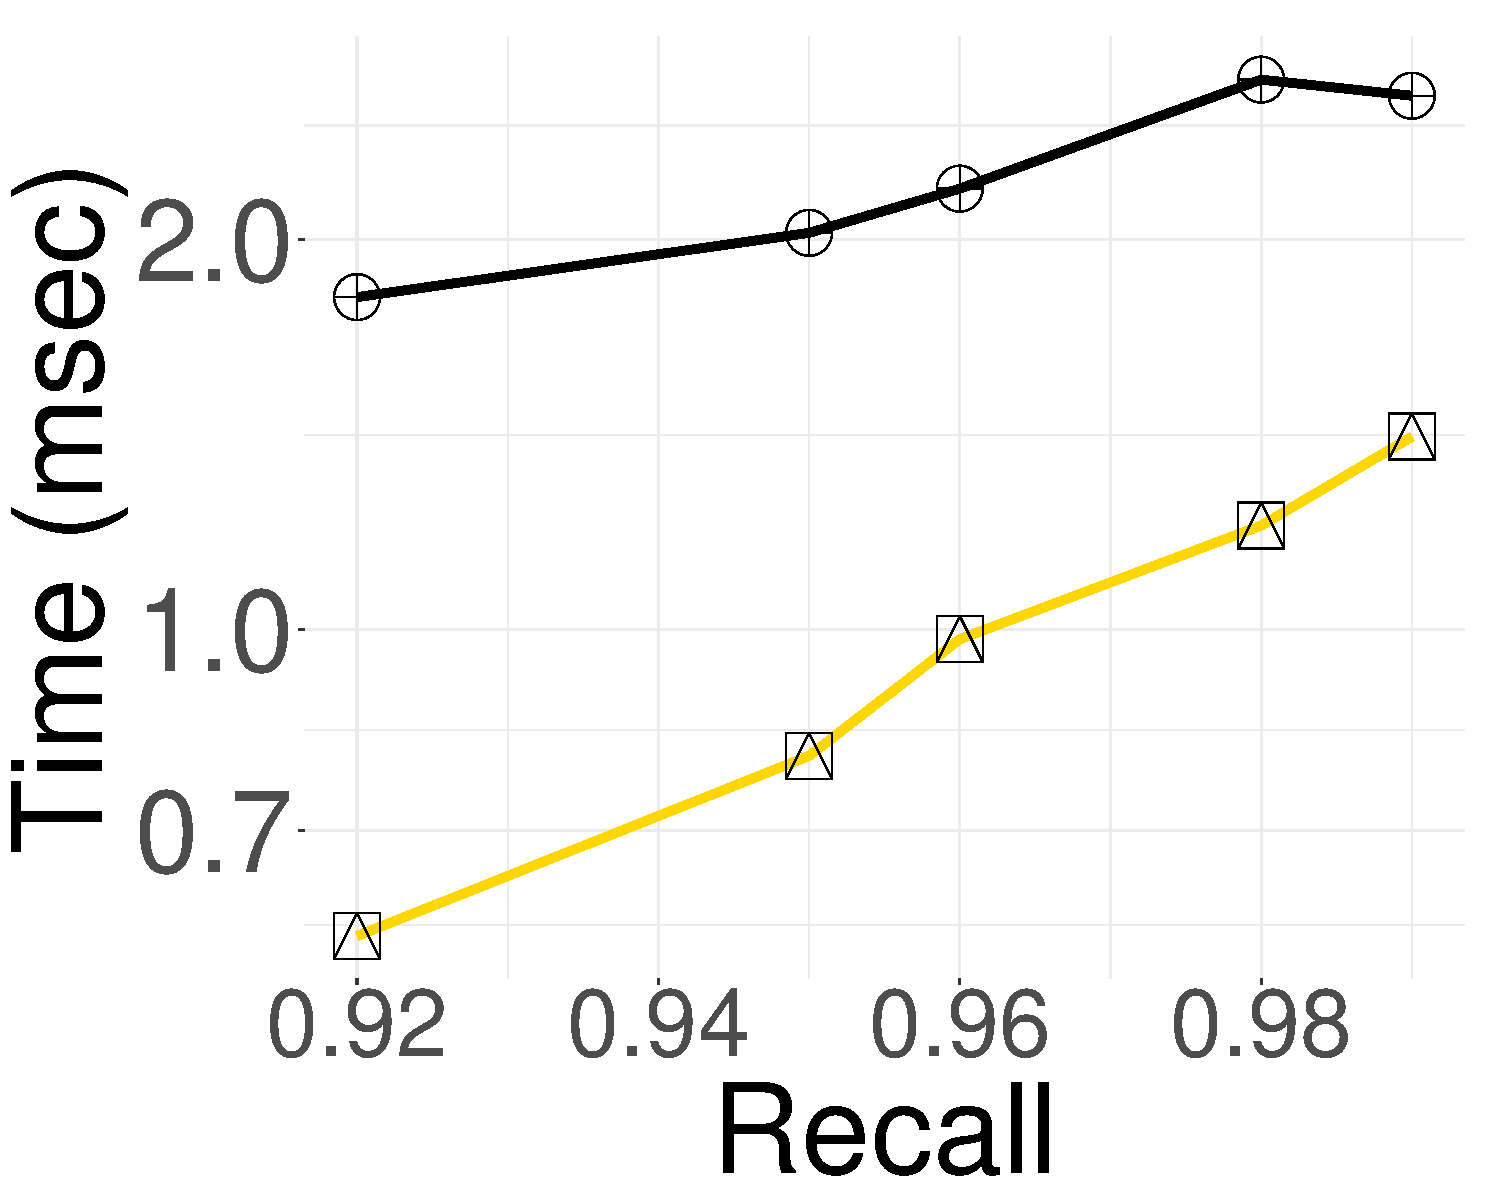
\includegraphics[width=\textwidth]{../img/oigas/PQVSPQS/100GB/deep_10_Time.pdf}
        \caption{Search Time (100GB)}
        \label{fig:SPQ:100GB_Time}
    \end{subfigure}
    \hspace{0.4cm}
    \begin{subfigure}[b]{0.28\textwidth}
        \captionsetup{justification=centering}
	\centering	
        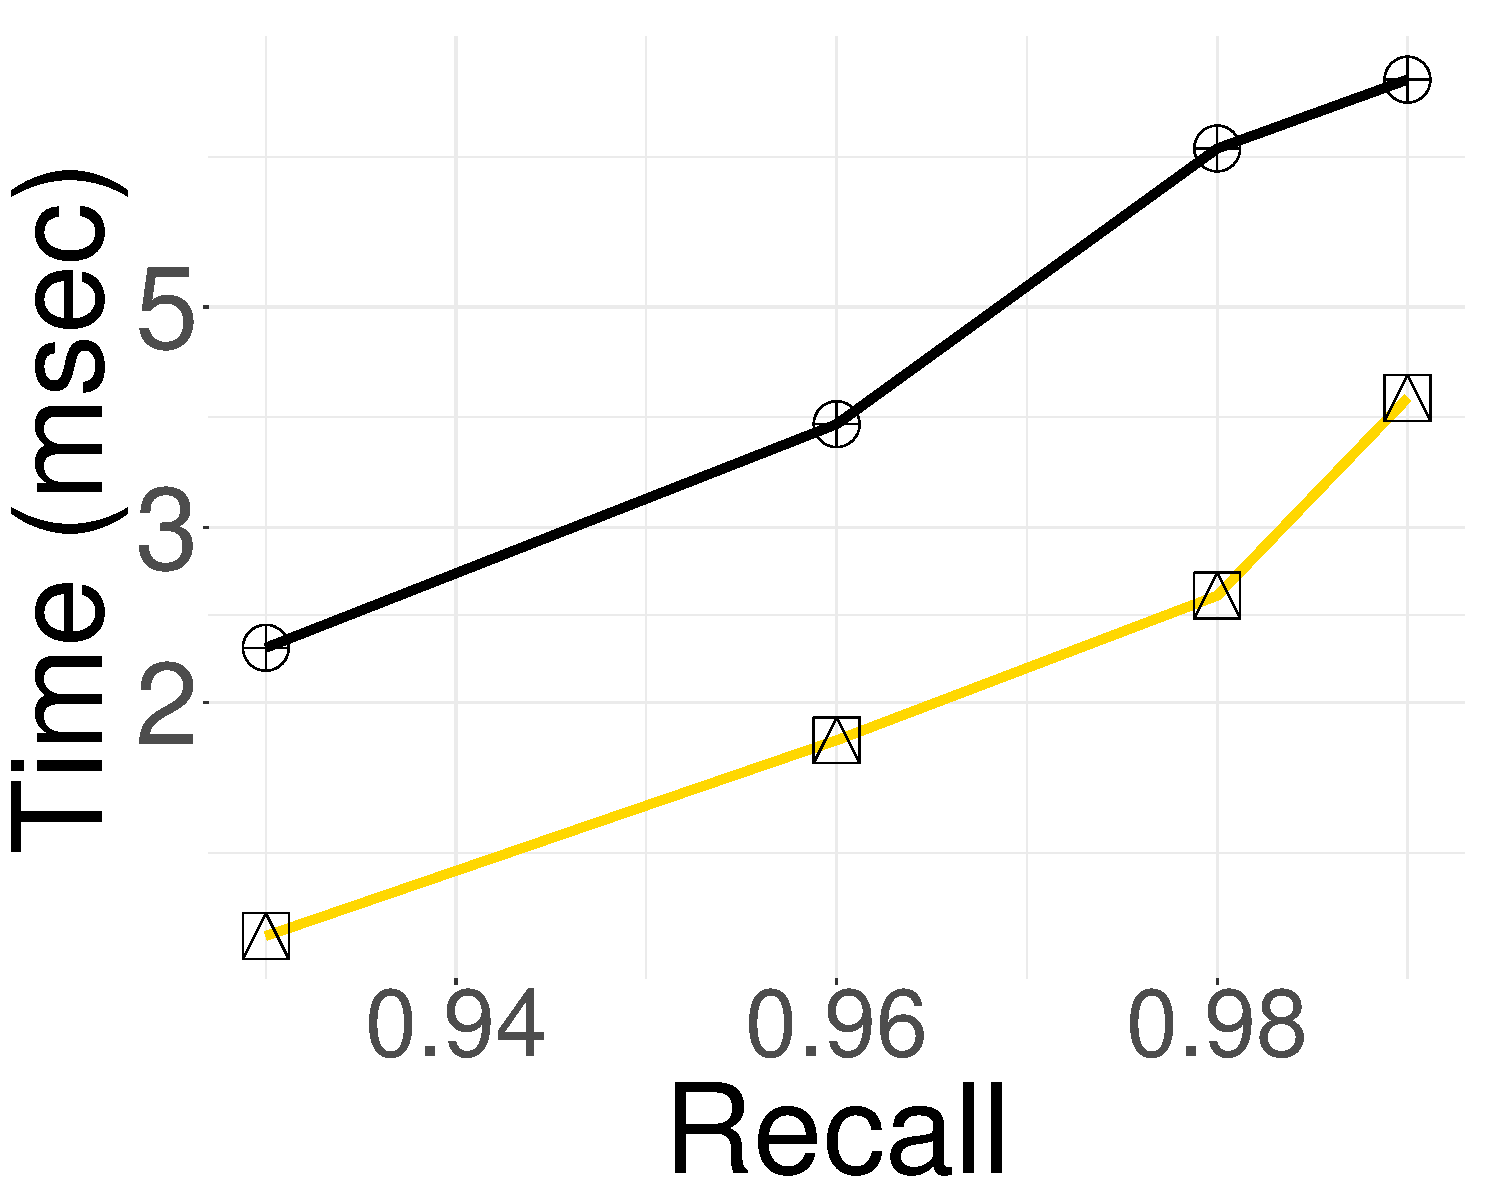
\includegraphics[width=\textwidth]{../img/oigas/PQVSPQS/1B/deep_10_Time.pdf}
        \caption{Search Time (1B)}
        \label{fig:SPQ:1B_Time}
    \end{subfigure}
    
    \begin{subfigure}[b]{0.28\textwidth}
        \captionsetup{justification=centering}
	\centering	
        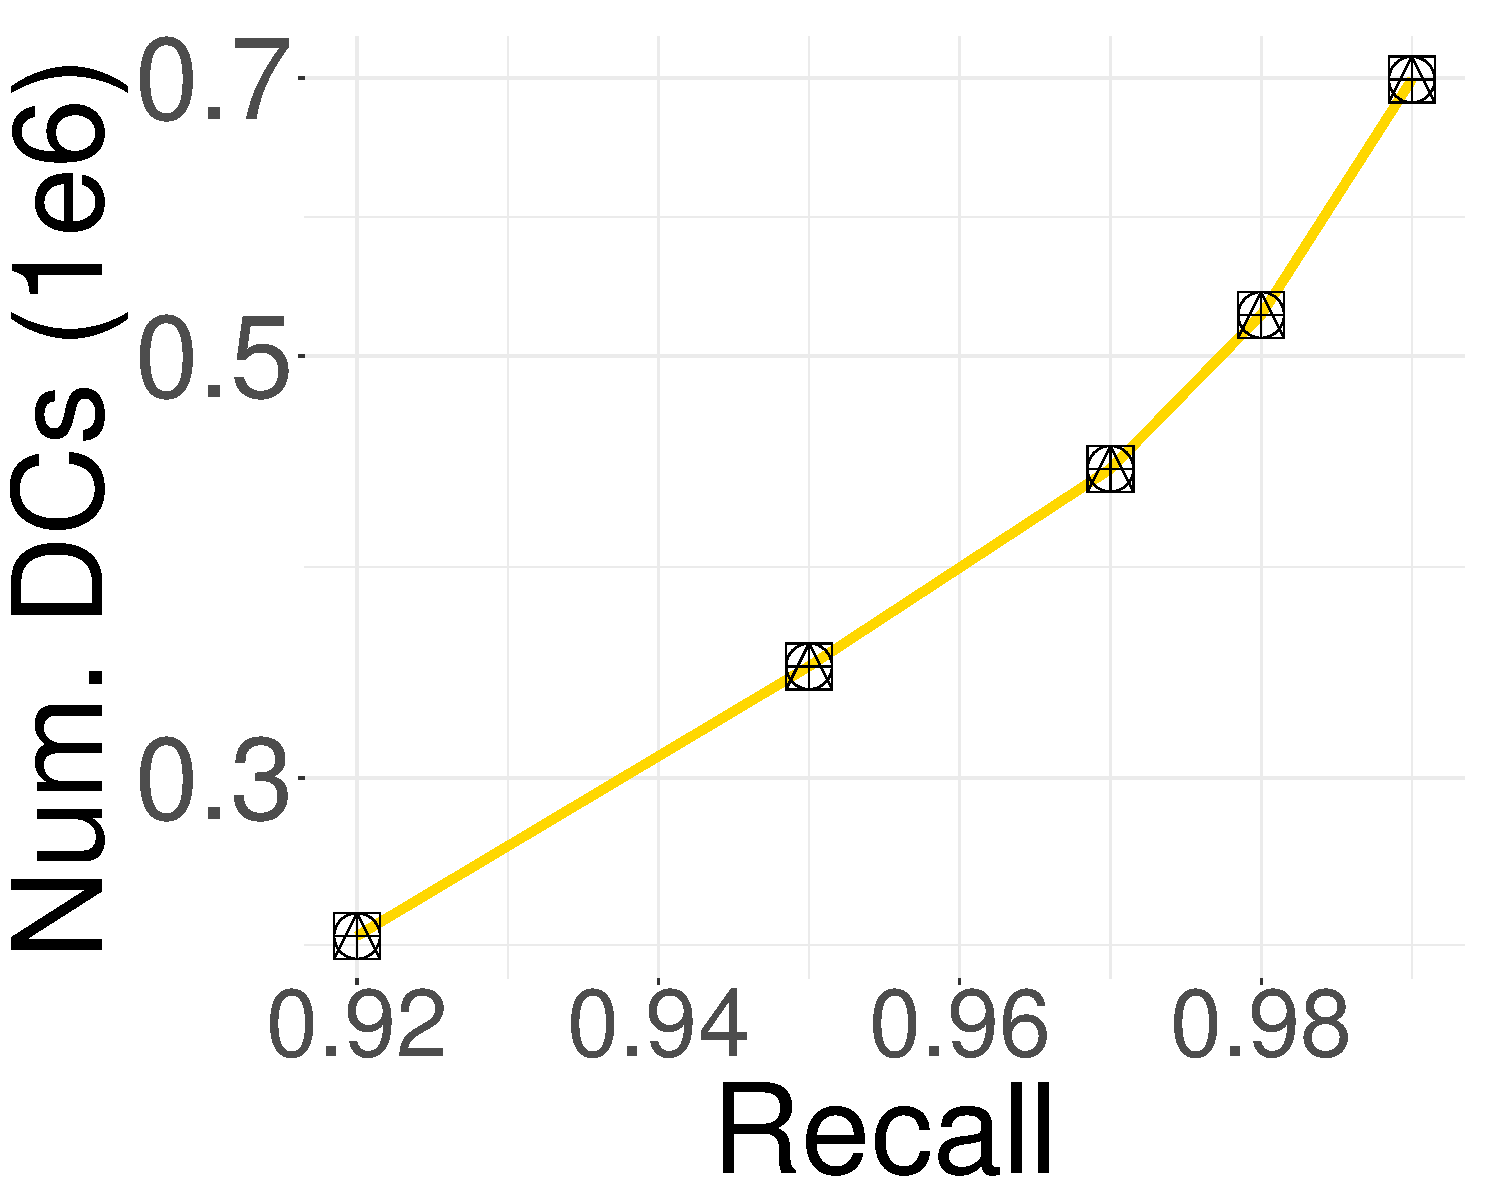
\includegraphics[width=\textwidth]{../img/oigas/PQVSPQS/25GB/deep_10_DC.pdf}
        \caption{Num. Dcs (25GB)}
        \label{fig:SPQ:25GB_DC}
    \end{subfigure}
    \hspace{0.4cm}
    \begin{subfigure}[b]{0.28\textwidth}
        \captionsetup{justification=centering}
	\centering	
        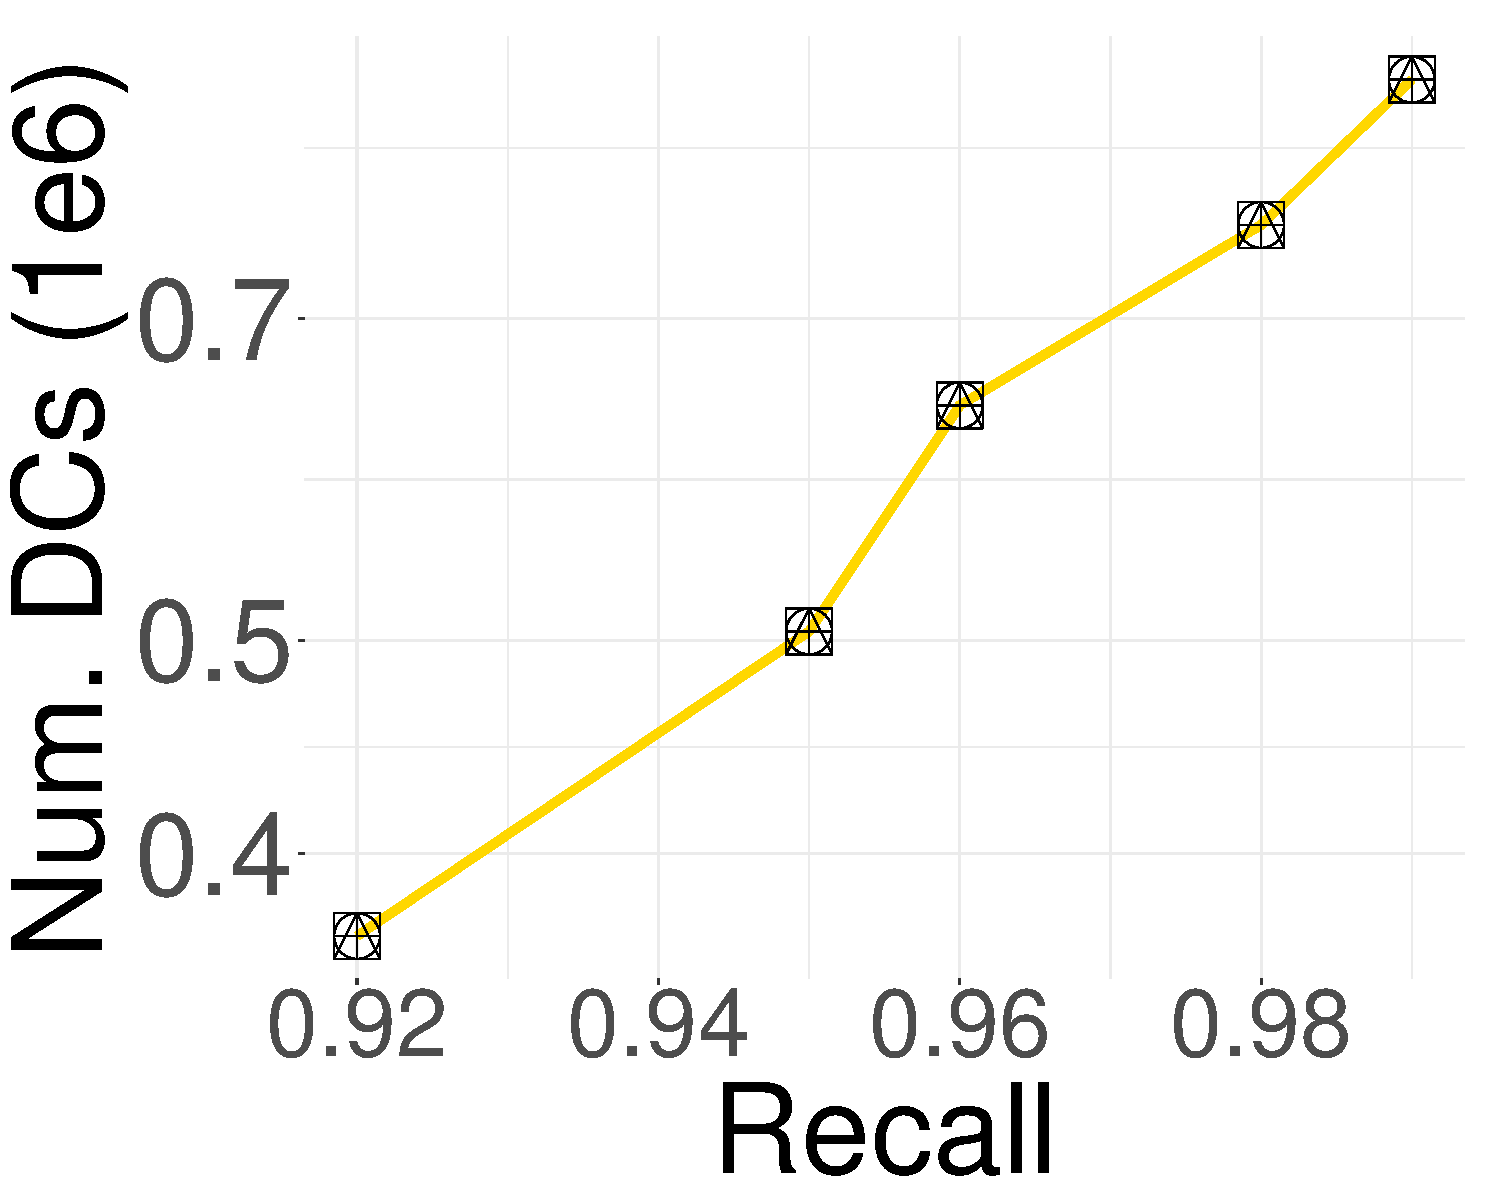
\includegraphics[width=\textwidth]{../img/oigas/PQVSPQS/100GB/deep_10_DC.pdf}
        \caption{Num. Dcs (100GB)}
        \label{fig:SPQ:100GB_DC}
    \end{subfigure}
    \hspace{0.4cm}
    \begin{subfigure}[b]{0.28\textwidth}
        \captionsetup{justification=centering}
	\centering	
        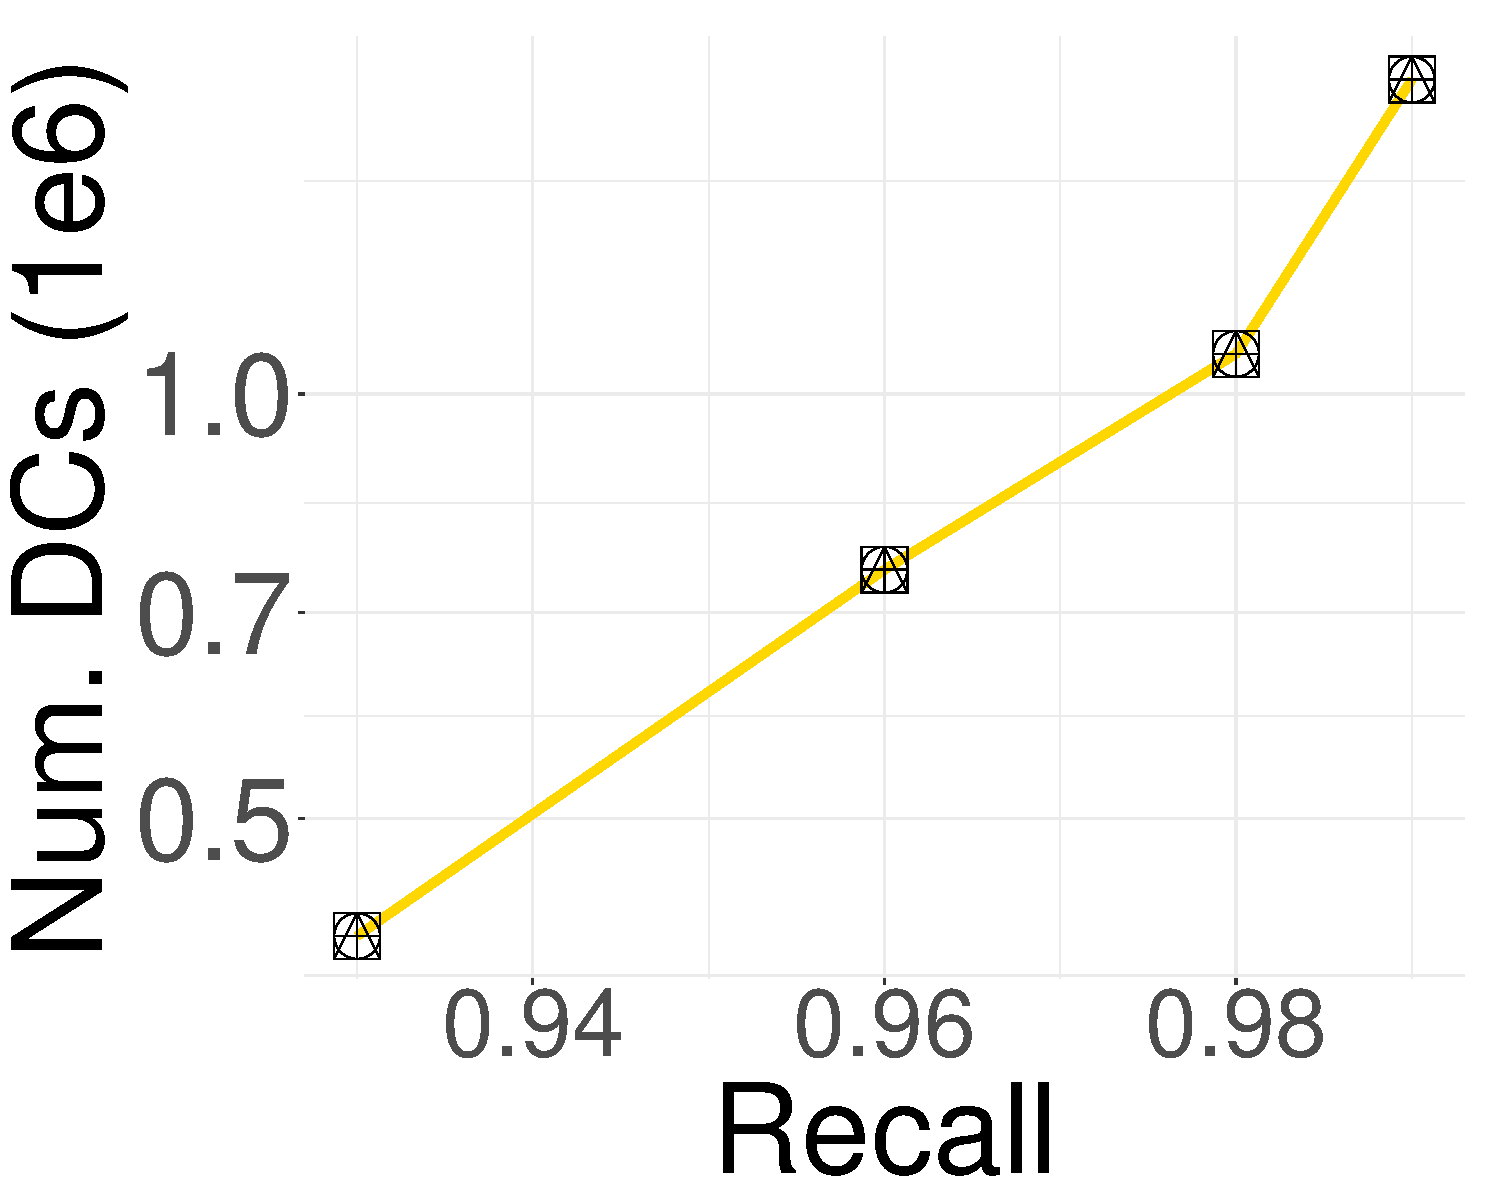
\includegraphics[width=\textwidth]{../img/oigas/PQVSPQS/1B/deep_10_DC.pdf}
        \caption{Num. Dcs (1B)}
        \label{fig:SPQ:1B_DC}
    \end{subfigure}
    \caption{Time and Number of distance calculations vs. accuracy on Deep1B dataset}
    \label{fig:hnswnew_time_and_dc}
\end{figure}

\subsection{SWB: Step-Wise Adaptive Beam Width}

We evaluate the effect of the Step-wise Adaptive Beam Width (SWB) approach on graph indexing efficiency and search performance. SWB is assessed using different numbers of steps, ranging from 2 to 6. When the number of steps is equal to 1, the beam width \( L \) remains fixed for all nodes, as in the original HNSW, which we refer to as Fixed Beam Width (FBW). For both FBW and SWB, we utilize the same graph indexing and search parameters across all runs to ensure a fair comparison.

\noindent{\textbf{Indexing.}} Figure~\ref{fig:oigas:swb:idx} illustrates the indexing time of FBW compared to SWB with varying numbers of steps. We observe that as the number of steps increases, the indexing time decreases by approximately 30 to 40\%. This improvement is attributed to the efficient adaptation of the beam width to the current size of early-inserted nodes. Specifically, as the graph size increases, the reduction in the number of distance calculations and indexing time remains significant, saving between 20\% and 30\% of indexing hours. This efficiency gain is particularly important for large-scale datasets, where substantial time savings translate to hours or even days when indexing billions of vectors.



\begin{figure}[htbp]
      \begin{subfigure}{0.028\textwidth}
        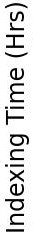
\includegraphics[width=\textwidth]{../img/oigas/CandNeighbors/legend_idx.jpg}
        \vspace{0.5cm}
        \label{fig:1M_Time}
    \end{subfigure}
     \centering
        \begin{subfigure}{0.31\textwidth}
            \captionsetup{justification=centering}
	\centering	
        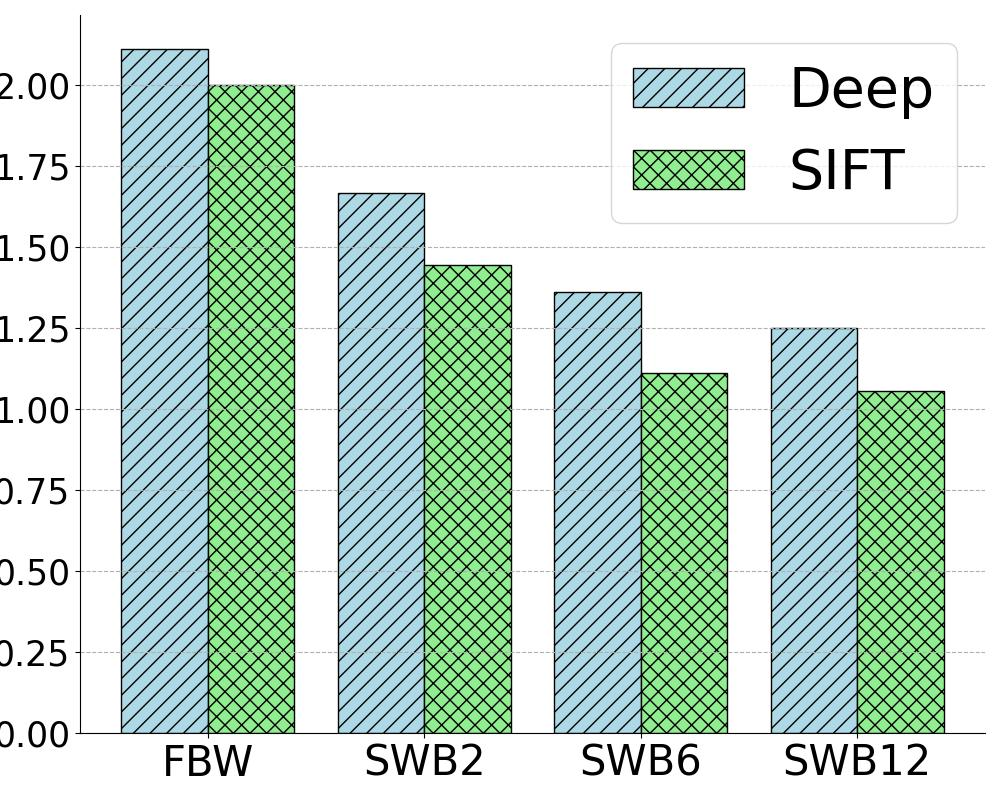
\includegraphics[width=\textwidth]{../img/oigas/SWB/25GB_Idx.jpg}
        \caption{25GB}
        \label{fig:SWB:25GB_Time}
    \end{subfigure}    
         \begin{subfigure}{0.31\textwidth}
             \captionsetup{justification=centering}
	\centering	
        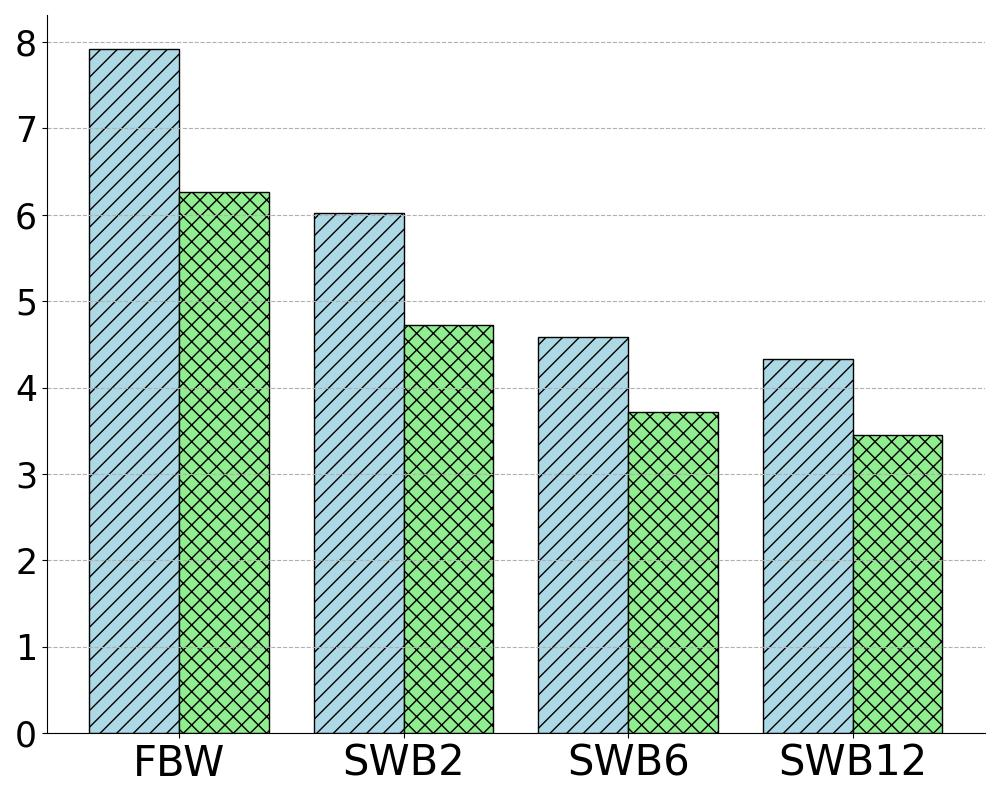
\includegraphics[width=\textwidth]{../img/oigas/SWB/100GB_Idx.jpg}
        \caption{100GB}
        \label{fig:SWB:100GB_Time}
    \end{subfigure}    
         \begin{subfigure}{0.31\textwidth}
             \captionsetup{justification=centering}
	\centering	
        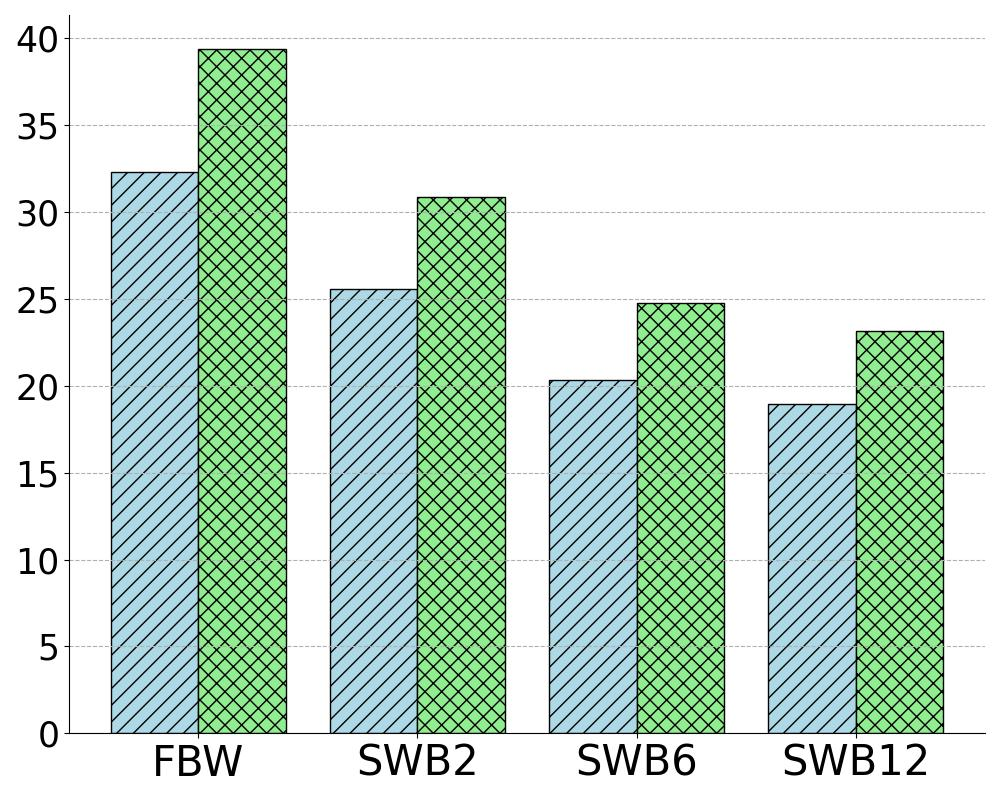
\includegraphics[width=\textwidth]{../img/oigas/SWB/1B_Idx.jpg}
        \caption{1B}
        \label{fig:SWB:1B_Time}
    \end{subfigure}
            \caption{Indexing Time using Step-wise Adaptive Beam Width}
            \label{fig:oigas:swb:idx}
    \end{figure}


\subsubsection{Search Performance}

Interestingly, applying Step-wise Adaptive Beam Width (SWB) during indexing not only reduces indexing time by up to 40\% but also enhances search efficiency. We conducted searches on graphs constructed using both Fixed Beam Width (FBW) and SWB. Our results in Figure~\ref{fig:SWBsearch} demonstrate that graphs generated with SWB incur fewer distance calculations during search as the number of steps increases.


\begin{figure}[ht]
    \centering
        \begin{subfigure}[b]{0.425\textwidth}
            \captionsetup{justification=centering}
	\centering	
        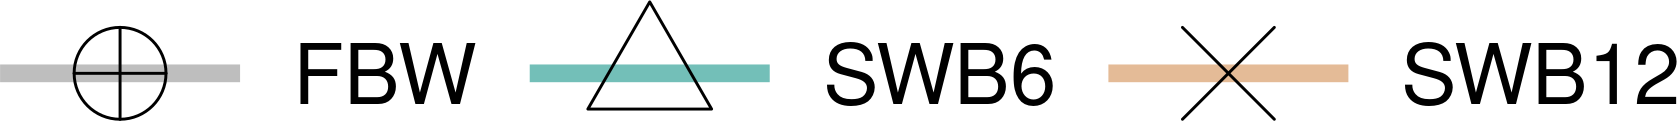
\includegraphics[width=\textwidth]{../img/oigas/SWB/search/legend.png}
    \end{subfigure}
  
        \begin{subfigure}[b]{0.28\textwidth}
            \captionsetup{justification=centering}
	\centering	
        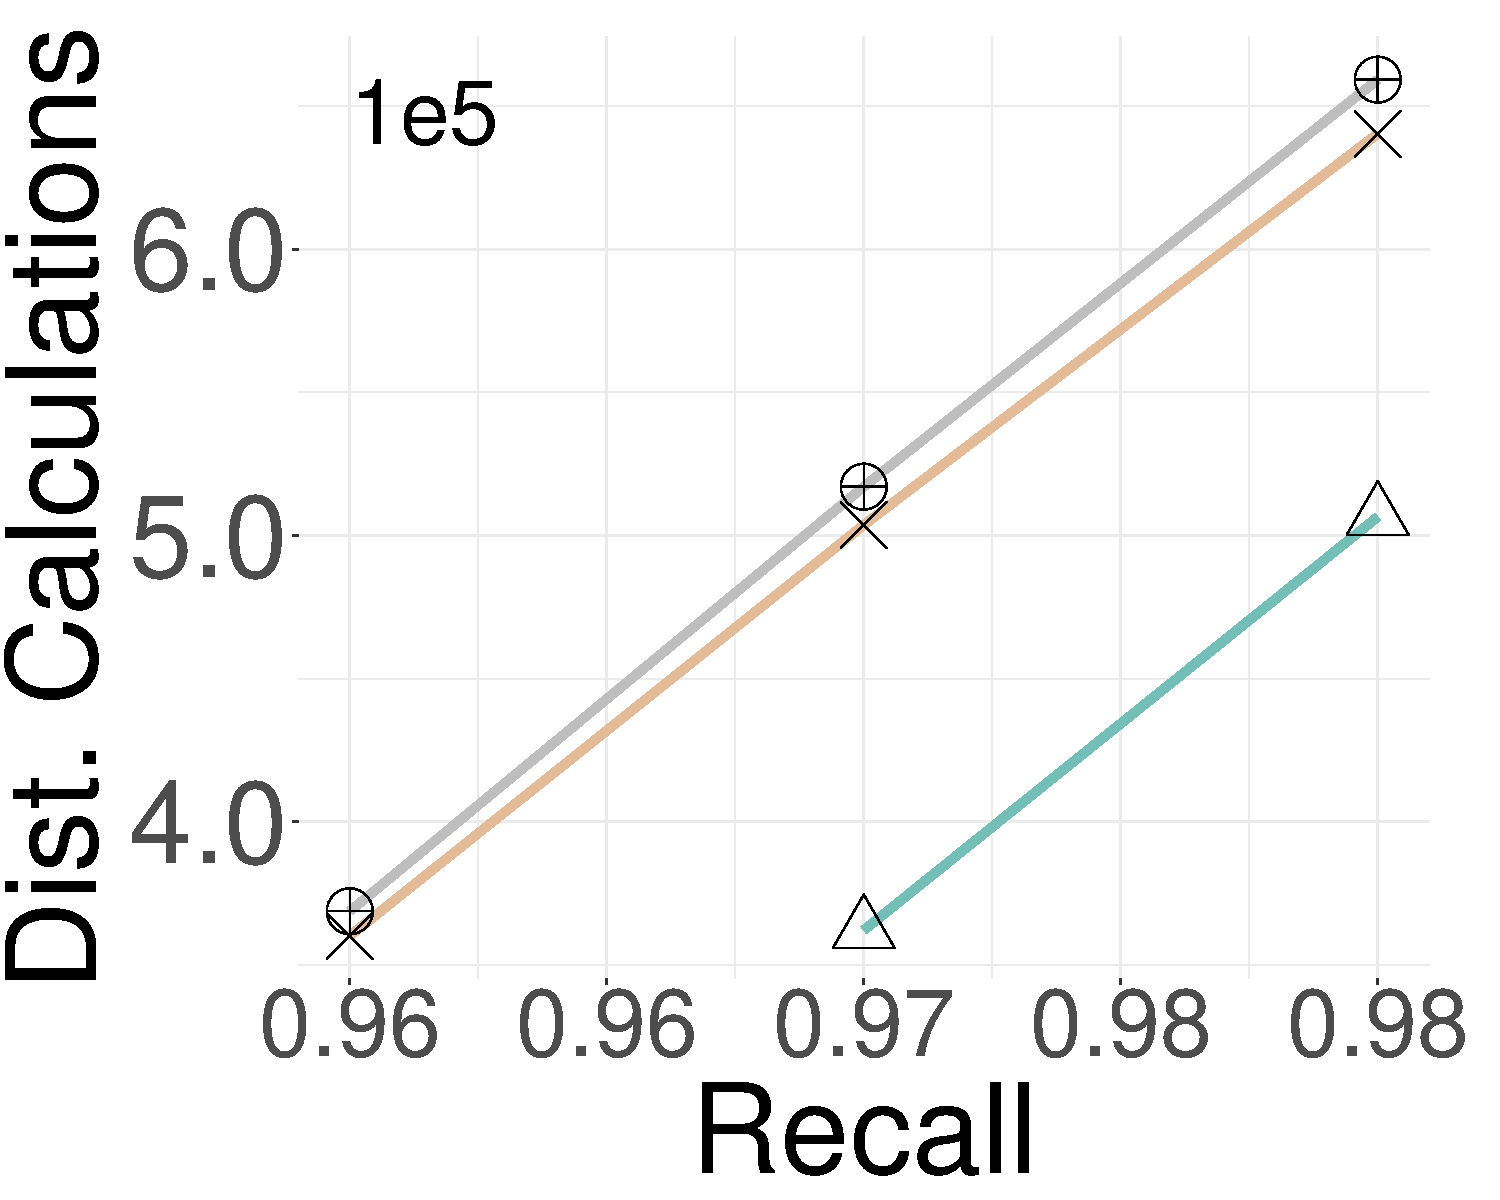
\includegraphics[width=\textwidth]{../img/oigas/SWB/search/25GB/deep_DC.pdf}
        \caption{Deep25GB}
        \label{fig:SWBsearch:_Time}
    \end{subfigure}
    \hspace{0.4cm}
            \begin{subfigure}[b]{0.28\textwidth}
                \captionsetup{justification=centering}
	\centering	
                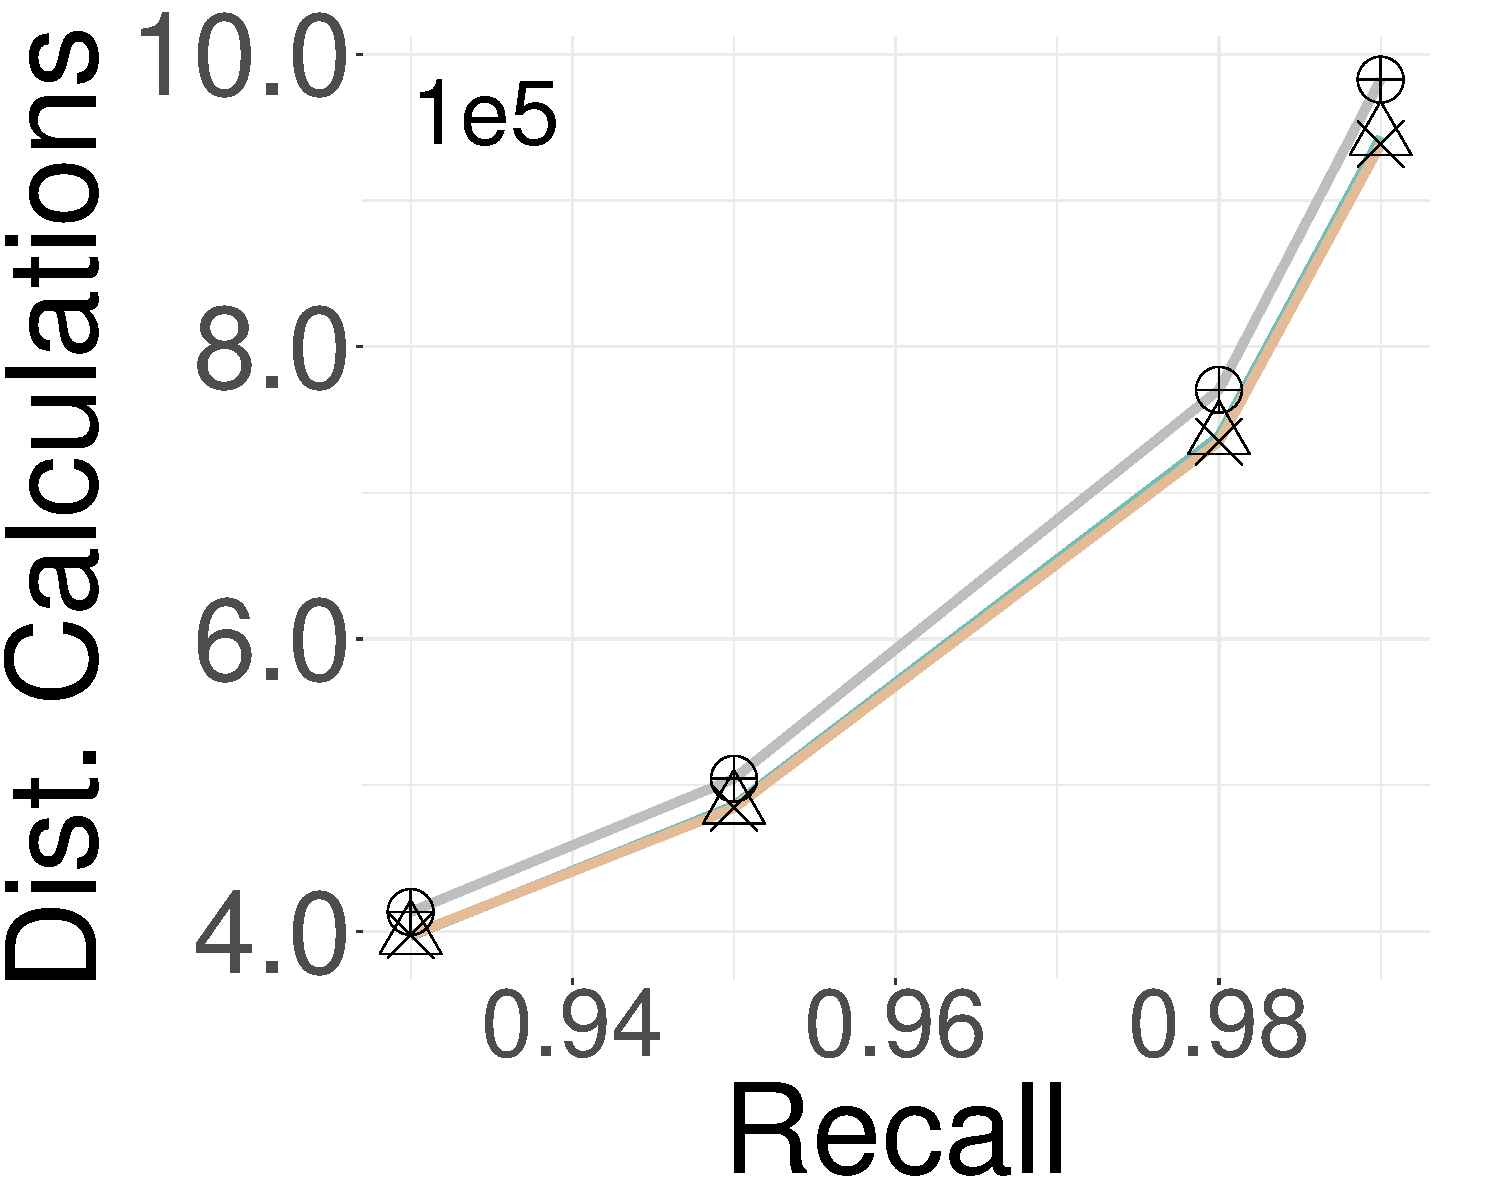
\includegraphics[width=\textwidth]{../img/oigas/SWB/search/100GB/deep_DC.pdf}
                \caption{Deep100GB}
        \label{fig:SWBsearch:_Time}
    \end{subfigure}
    \hspace{0.4cm}
             \begin{subfigure}[b]{0.28\textwidth}
                 \captionsetup{justification=centering}
	\centering	
                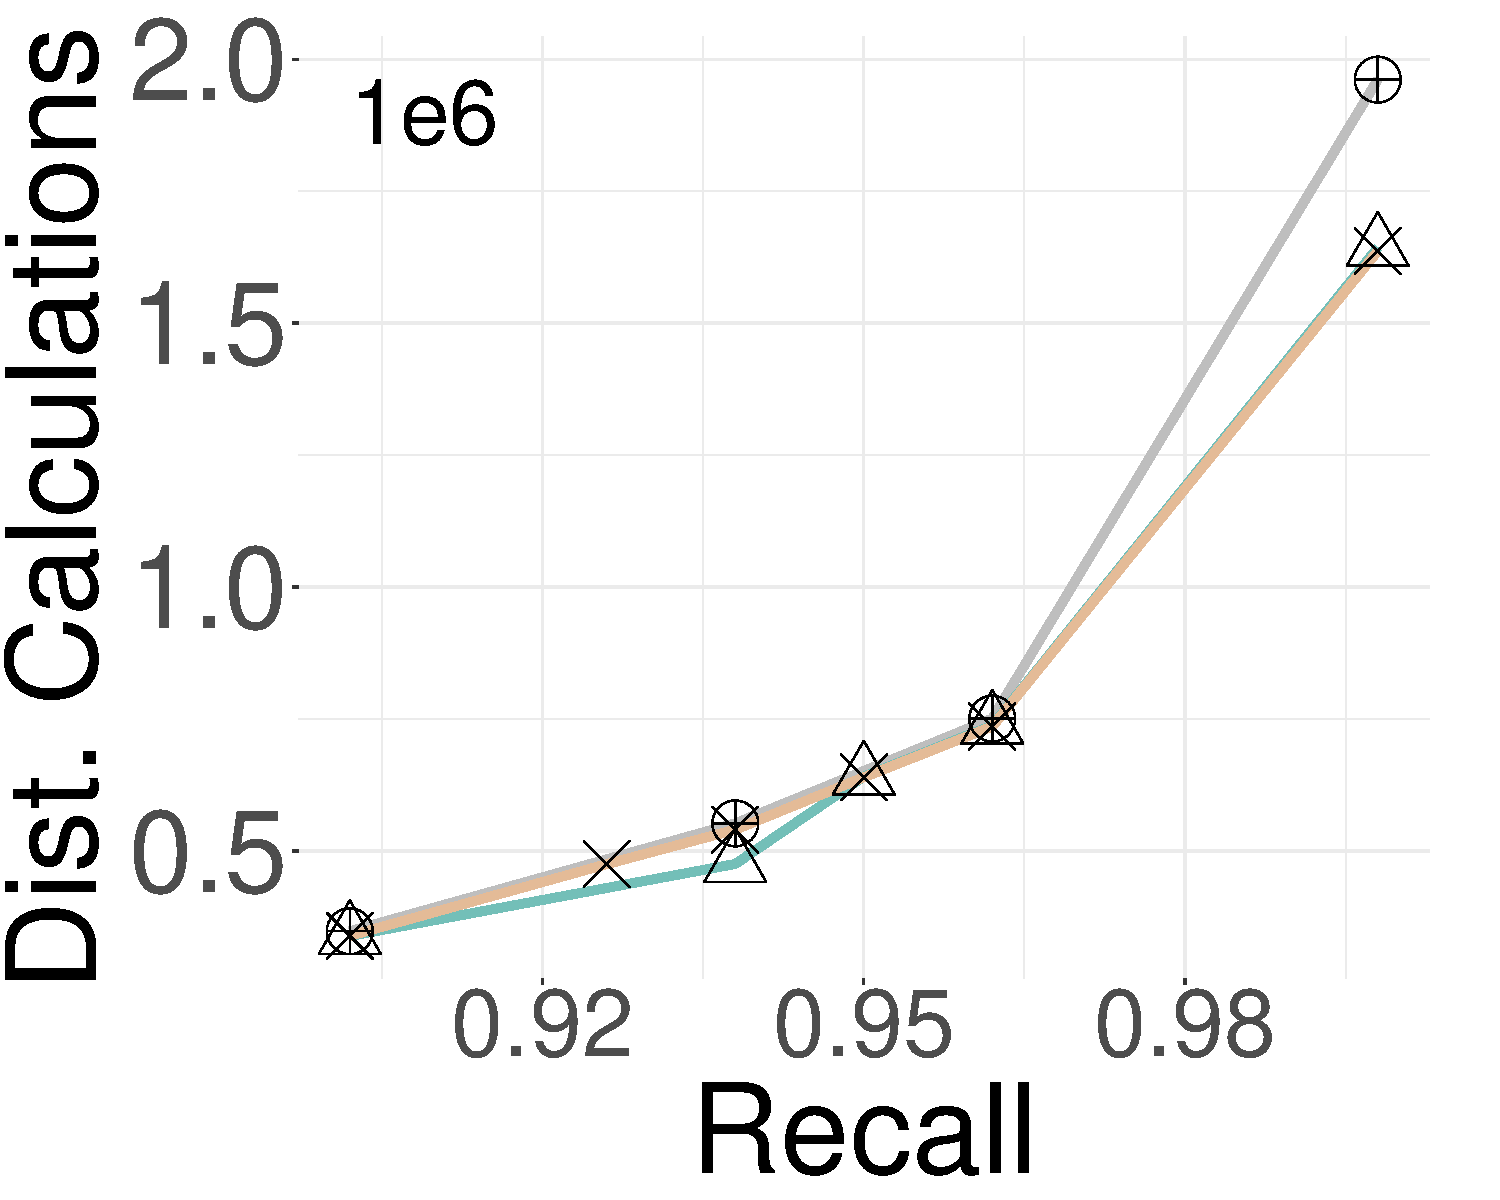
\includegraphics[width=\textwidth]{../img/oigas/SWB/search/1B/deep_DC.pdf}
        \caption{Deep1B}
        \label{fig:SWBsearch:_Time}
    \end{subfigure}

          \begin{subfigure}[b]{0.28\textwidth}
              \captionsetup{justification=centering}
	\centering	
        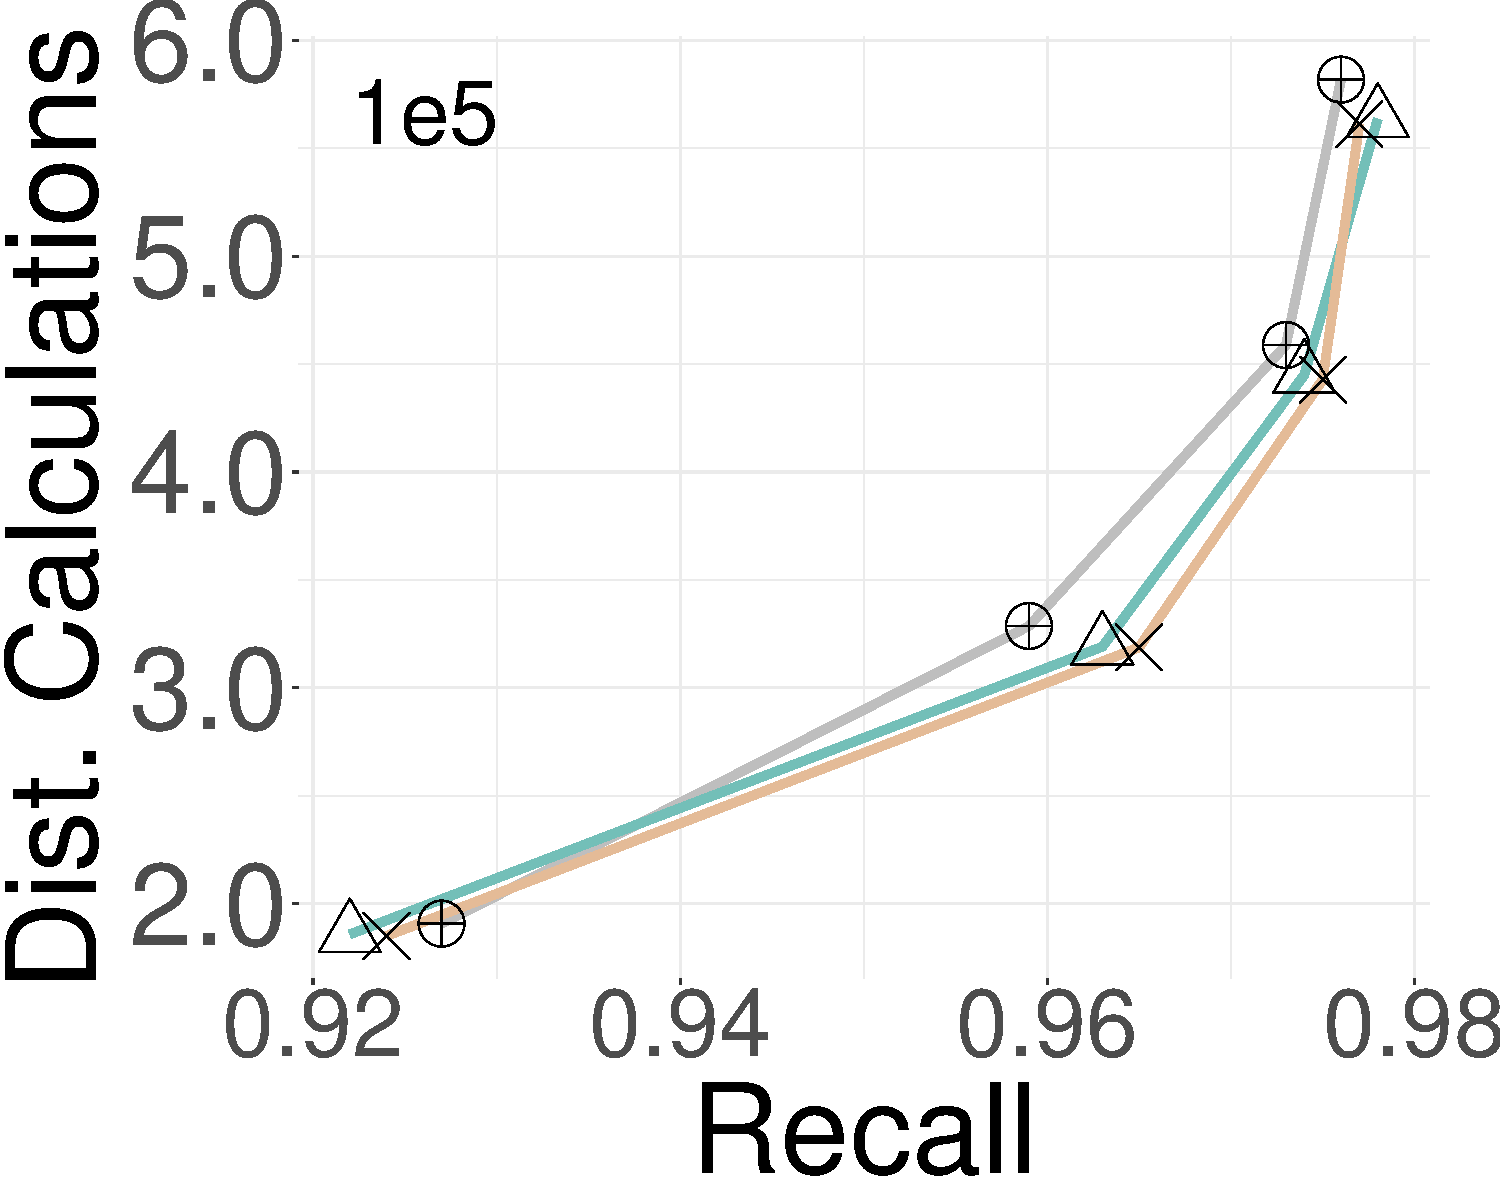
\includegraphics[width=\textwidth]{../img/oigas/SWB/search/25GB/sift_DC.pdf}
        \caption{Sift25GB}
        \label{fig:SWBsearch:_Time}
    \end{subfigure}
    \hspace{0.4cm}
            \begin{subfigure}[b]{0.28\textwidth}
                \captionsetup{justification=centering}
	\centering	
                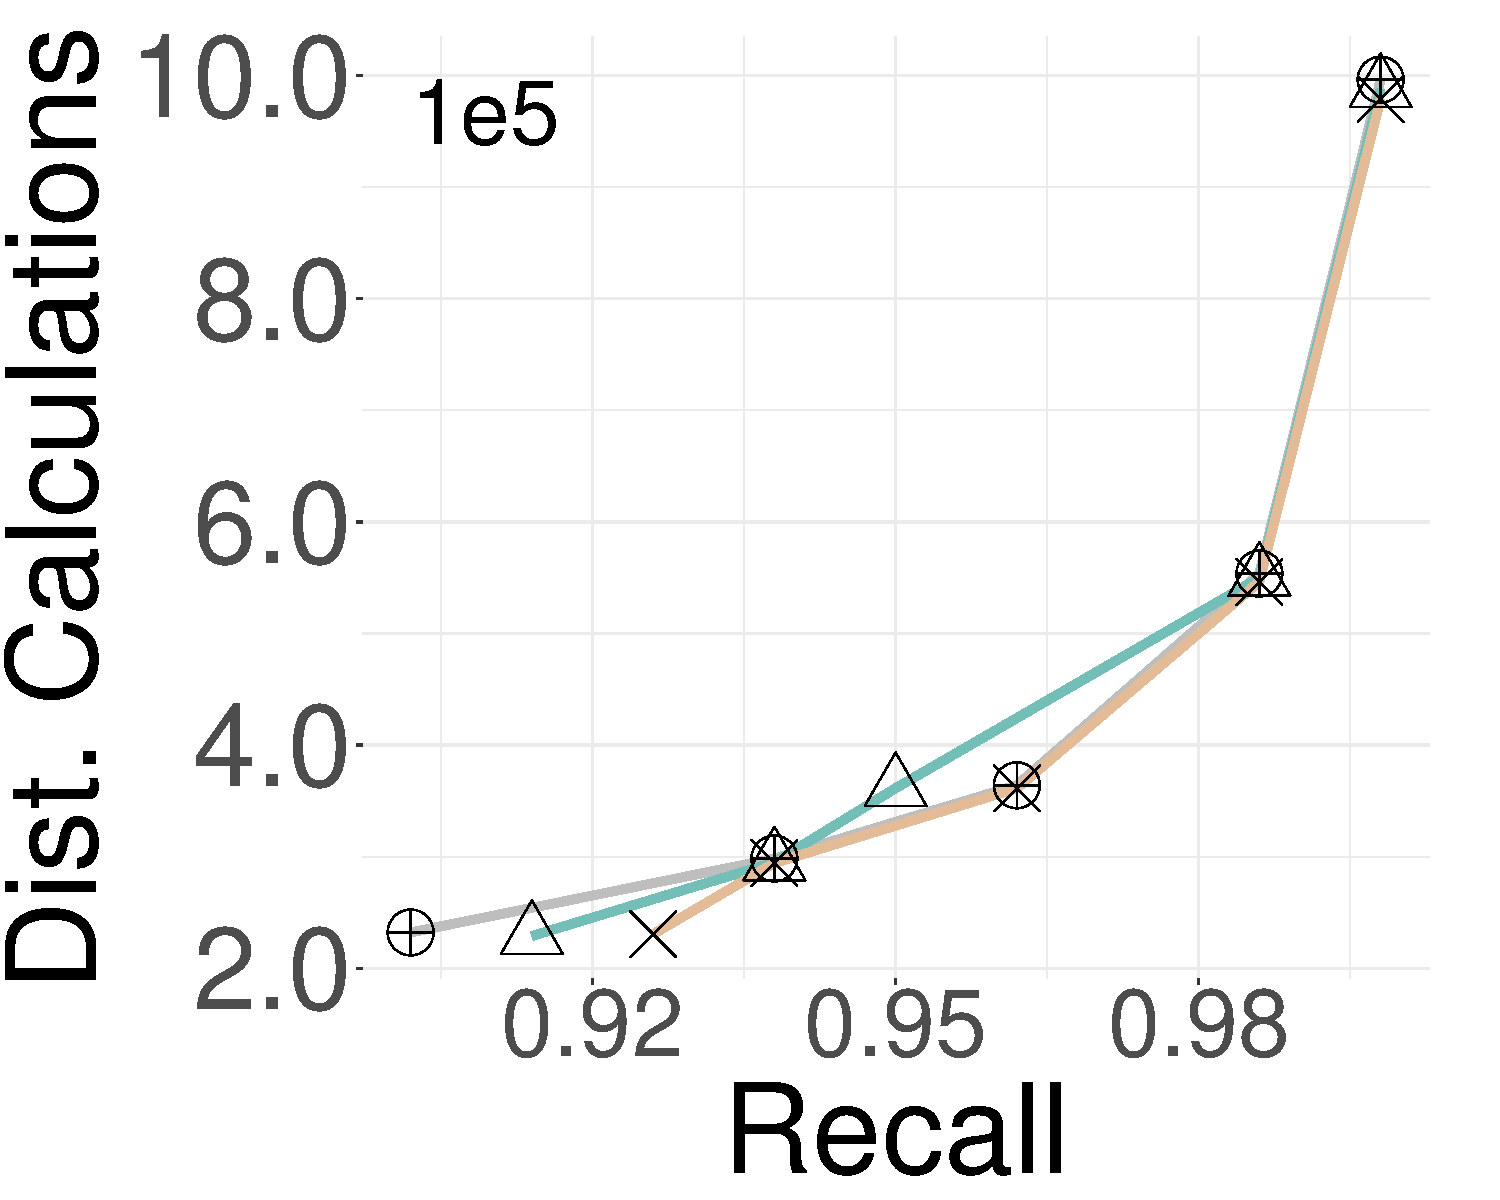
\includegraphics[width=\textwidth]{../img/oigas/SWB/search/100GB/sift_DC.pdf}
                \caption{Sift100GB}
        \label{fig:SWBsearch:_Time}
    \end{subfigure}
    \hspace{0.4cm}
             \begin{subfigure}[b]{0.28\textwidth}
                 \captionsetup{justification=centering}
	\centering	
                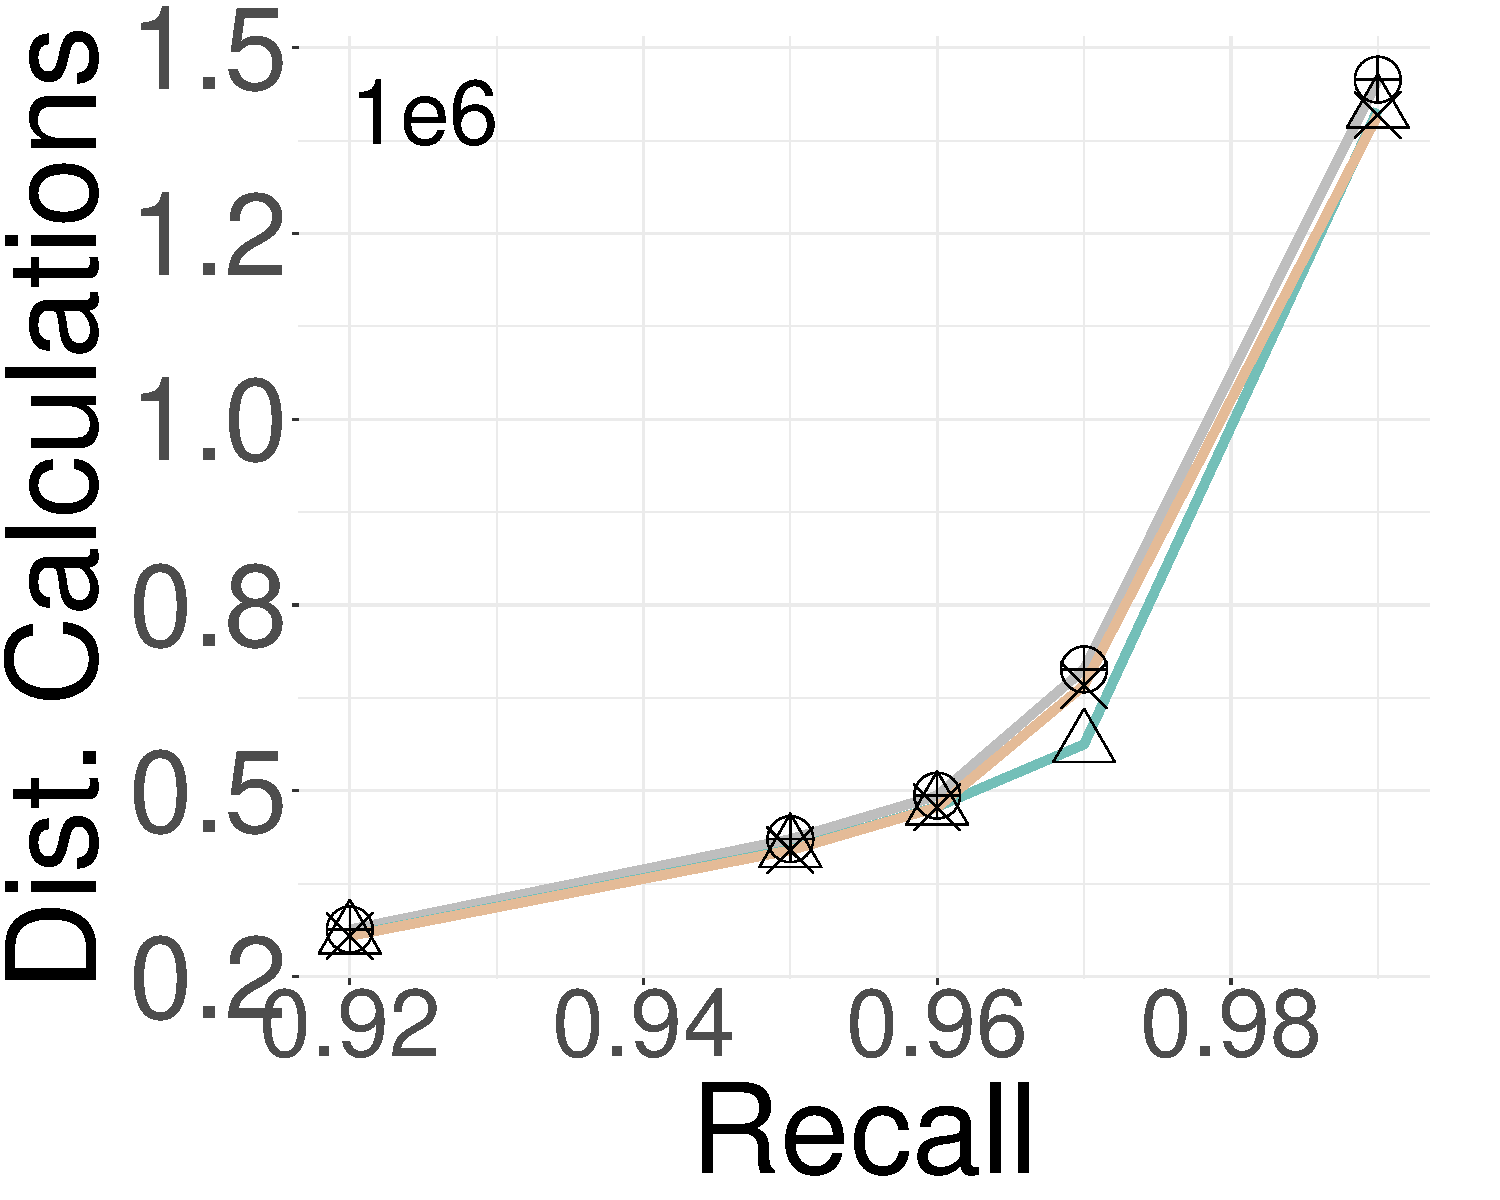
\includegraphics[width=\textwidth]{../img/oigas/SWB/search/1B/sift_DC.pdf}
        \caption{Sift1B}
        \label{fig:SWBsearch:_Time}
    \end{subfigure}
    \caption{Search performance of different SWB methodes based graph on Deep and Sift datasets}
    \label{fig:SWBsearch}
\end{figure}

A valid and reasonable explanation for this phenomenon relates to the graph's outdegree. When applying Step-wise Adaptive Beam Width (SWB), the average outdegree of the graph is reduced by 3 to 5\%. We assume that reducing the beam width \( L \) for early nodes helps decrease the size of the candidate set in step (1). This reduction impacts the outdegree because a high beam width retrieves more candidates from the nearest neighbor (NN) regions of the nodes. Under the assumption that the pruning ratio is uniform across the candidate neighbor sets of all nodes, some nodes will restrict their neighborhood connections to a few, while only nodes with high in-degree will maintain more connections. These findings are noteworthy in our analysis, and we aim to study their effects further in future work.

\subsection{Combined Neighborhood Diversification Approach}

We evaluate the combined Neighborhood Diversification (ND) approaches, RND and RRND, during node insertion for both pruning stages (2) and (4) against the ND approaches employed in state-of-the-art methods, including RND, RRND, MOND, and NOND.

\begin{figure}[ht]
	\captionsetup{justification=centering}
	\centering	
		\begin{subfigure}{\columnwidth}
			\centering
			\captionsetup{justification=centering}	
			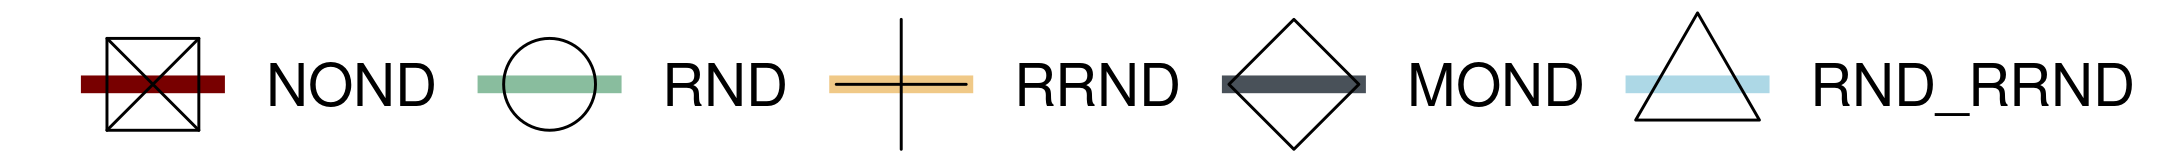
\includegraphics[width=0.6\columnwidth]{../img/oigas/RND_RRND/legend.png}
		\end{subfigure}\\
		\begin{subfigure}{0.28\columnwidth}
			\centering
			\captionsetup{justification=centering}	
			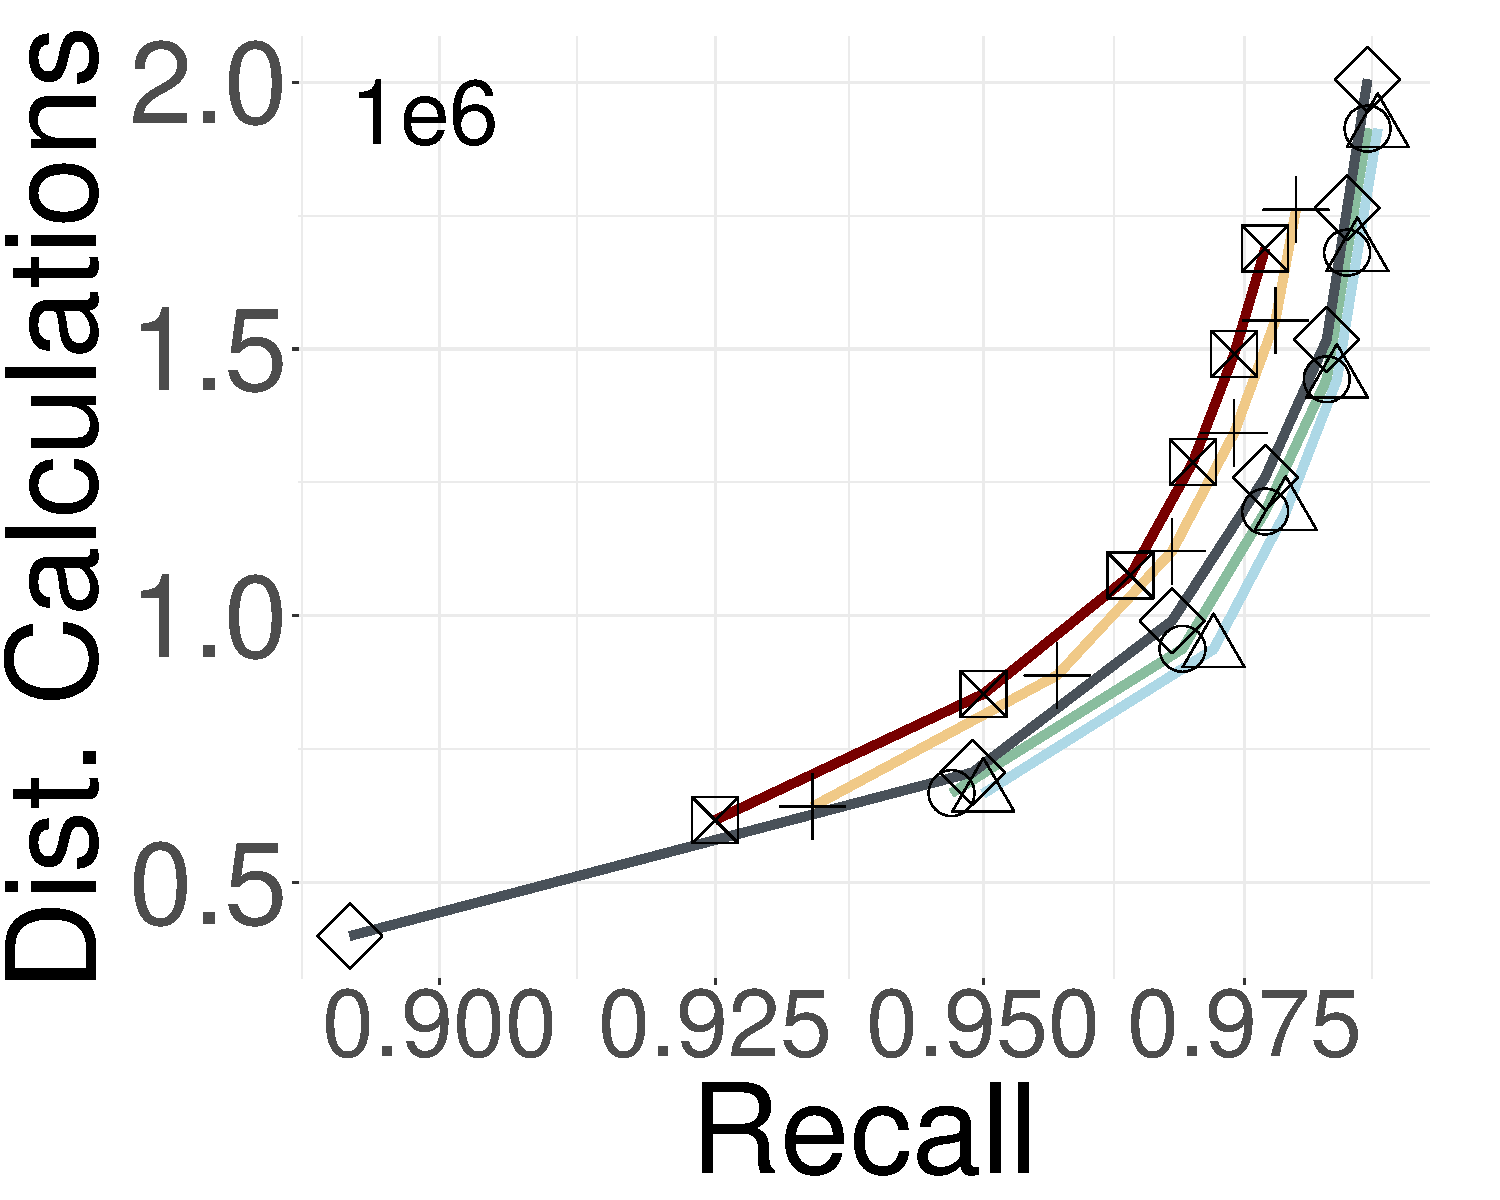
\includegraphics[width=\textwidth]{../img/oigas/RND_RRND/DC_DEEP25GB.pdf}
		\caption{{Deep25GB}}
		\label{fig:ND:deep25GB}	
		\end{subfigure}	
  \hspace{0.4cm}
		\begin{subfigure}{0.28\columnwidth}
			\centering
			\captionsetup{justification=centering}	
			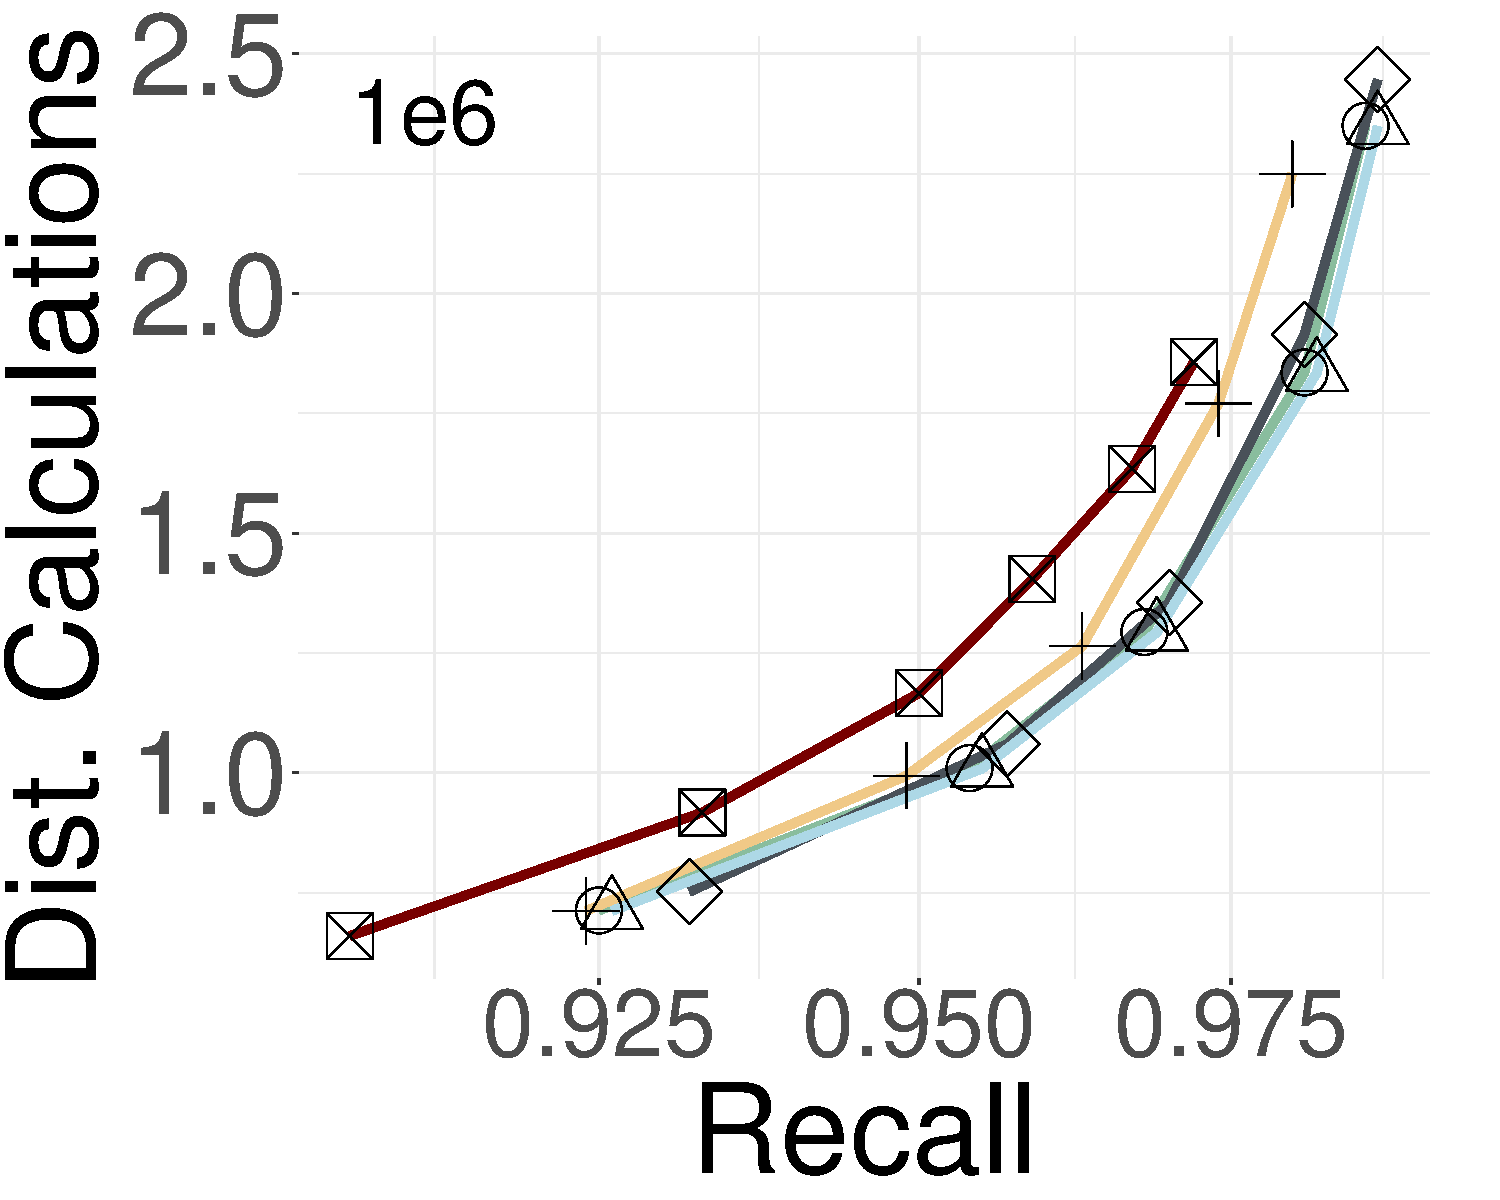
\includegraphics[width=\textwidth]{../img/oigas/RND_RRND/DC_DEEP100GB.pdf}
		\caption{{Deep100GB}}
		\label{fig:ND:deep100GB}
		\end{subfigure}	
  \hspace{0.4cm}
		\begin{subfigure}{0.28\columnwidth}
			\centering
			\captionsetup{justification=centering}	
			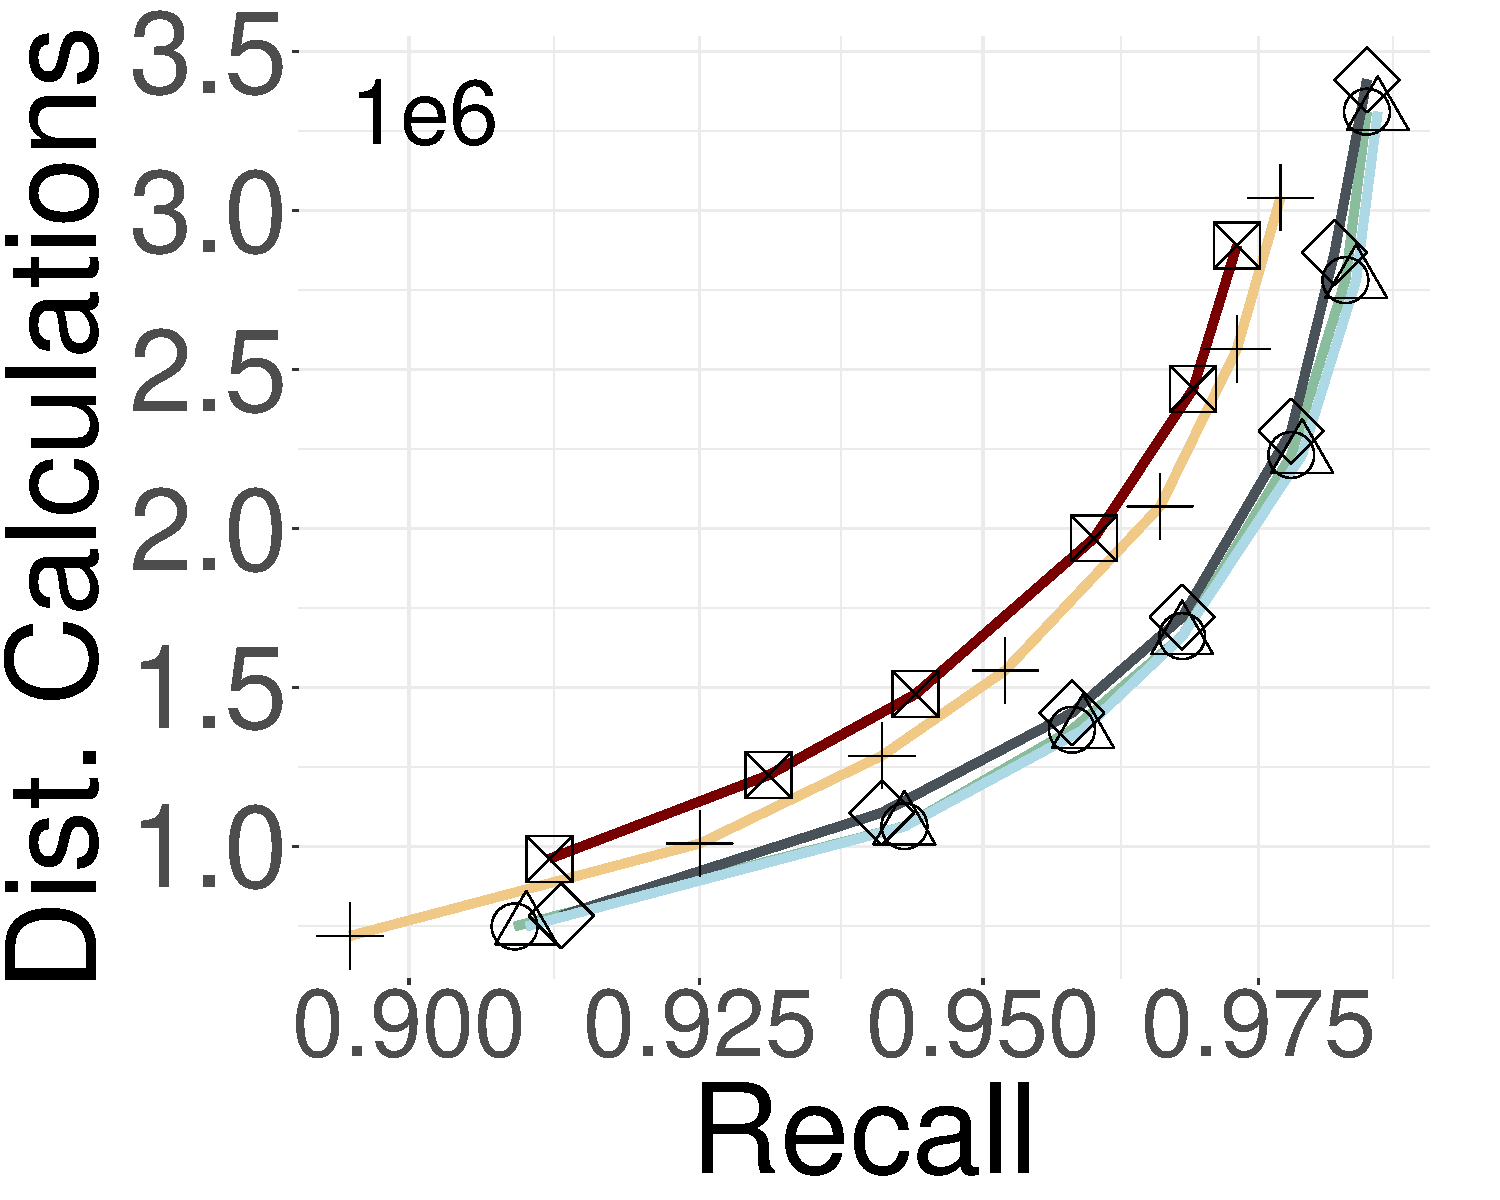
\includegraphics[width=\textwidth]{../img/oigas/RND_RRND/DC_DEEP1B.pdf}
		\caption{{Deep1B}}%need to be updated
		\label{fig:ND:deep1b}	
  \end{subfigure}	
		\begin{subfigure}{0.28\columnwidth}
			\centering
			\captionsetup{justification=centering}	
			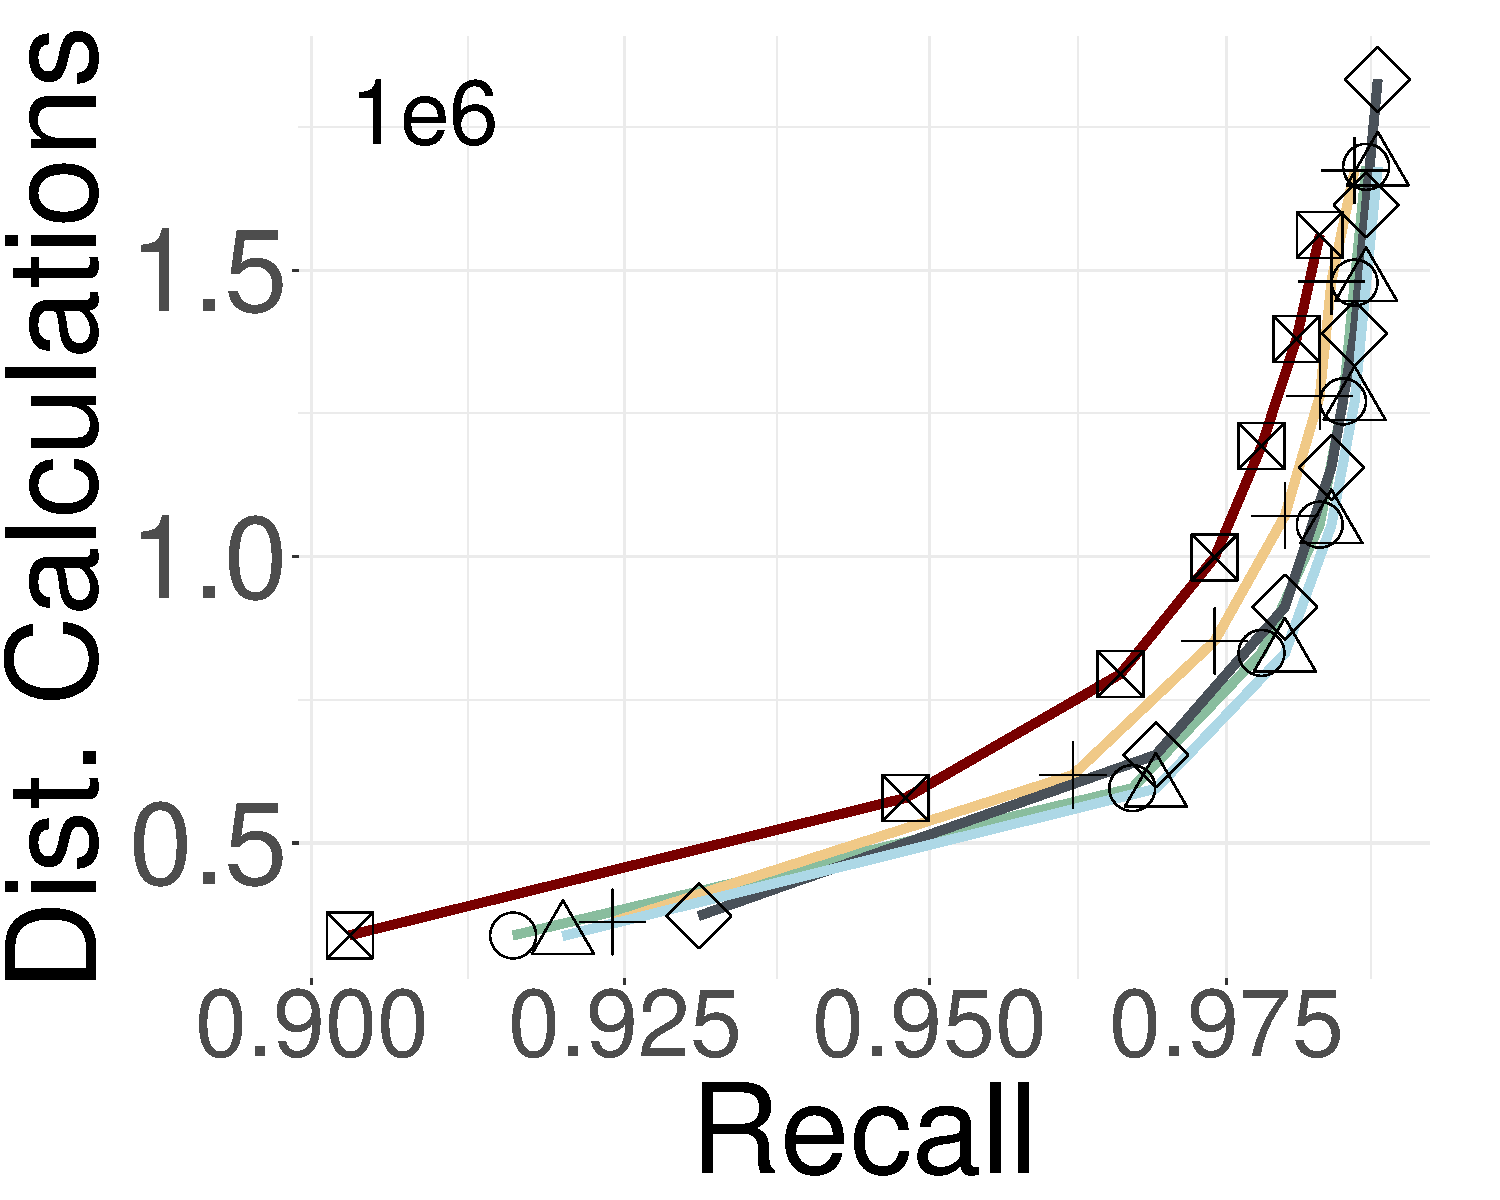
\includegraphics[width=\textwidth]{../img/oigas/RND_RRND/DC_SIFT25GB.pdf}
   \caption{{Sift25GB}}
		\label{fig:ND:sift25GB}
		\end{subfigure}	
  \hspace{0.4cm}
		\begin{subfigure}{0.28\columnwidth}
			\centering
			\captionsetup{justification=centering}	
			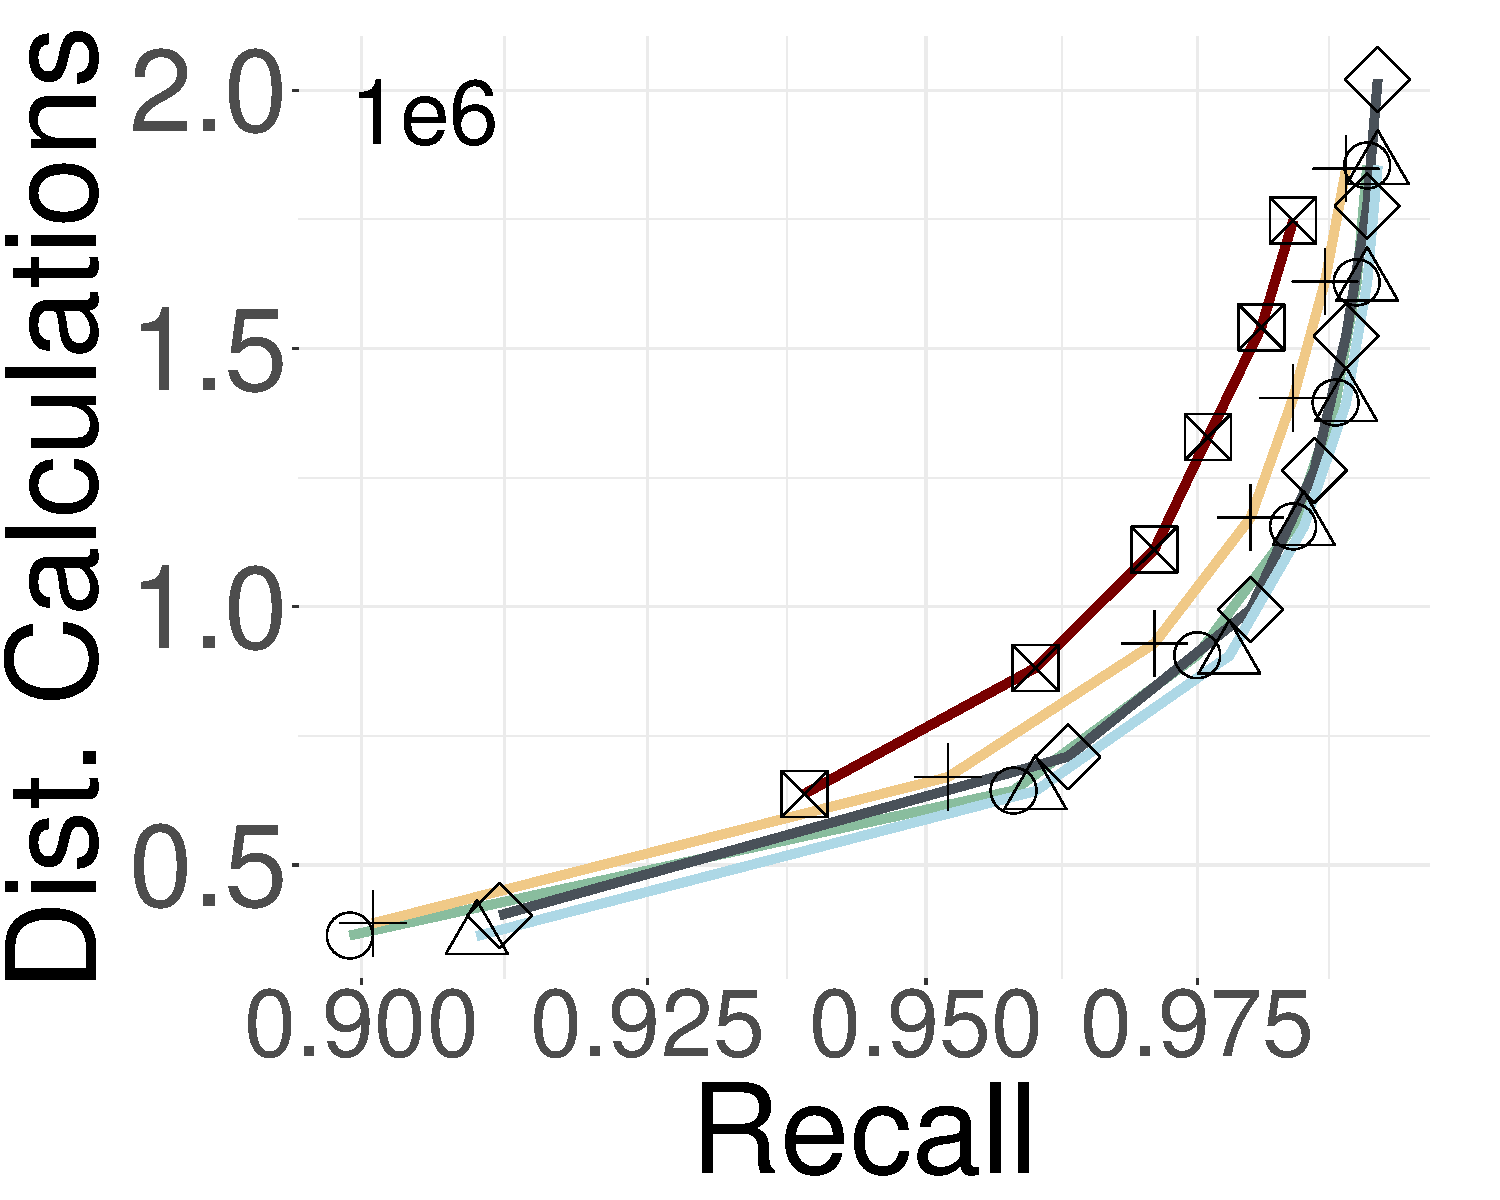
\includegraphics[width=\textwidth]{../img/oigas/RND_RRND/DC_SIFT100GB.pdf}
             \caption{{Sift100GB}}
		      \label{fig:ND:sift100GB}
		\end{subfigure}	
  \hspace{0.4cm}
		\begin{subfigure}{0.28\columnwidth}
			\centering
			\captionsetup{justification=centering}	
			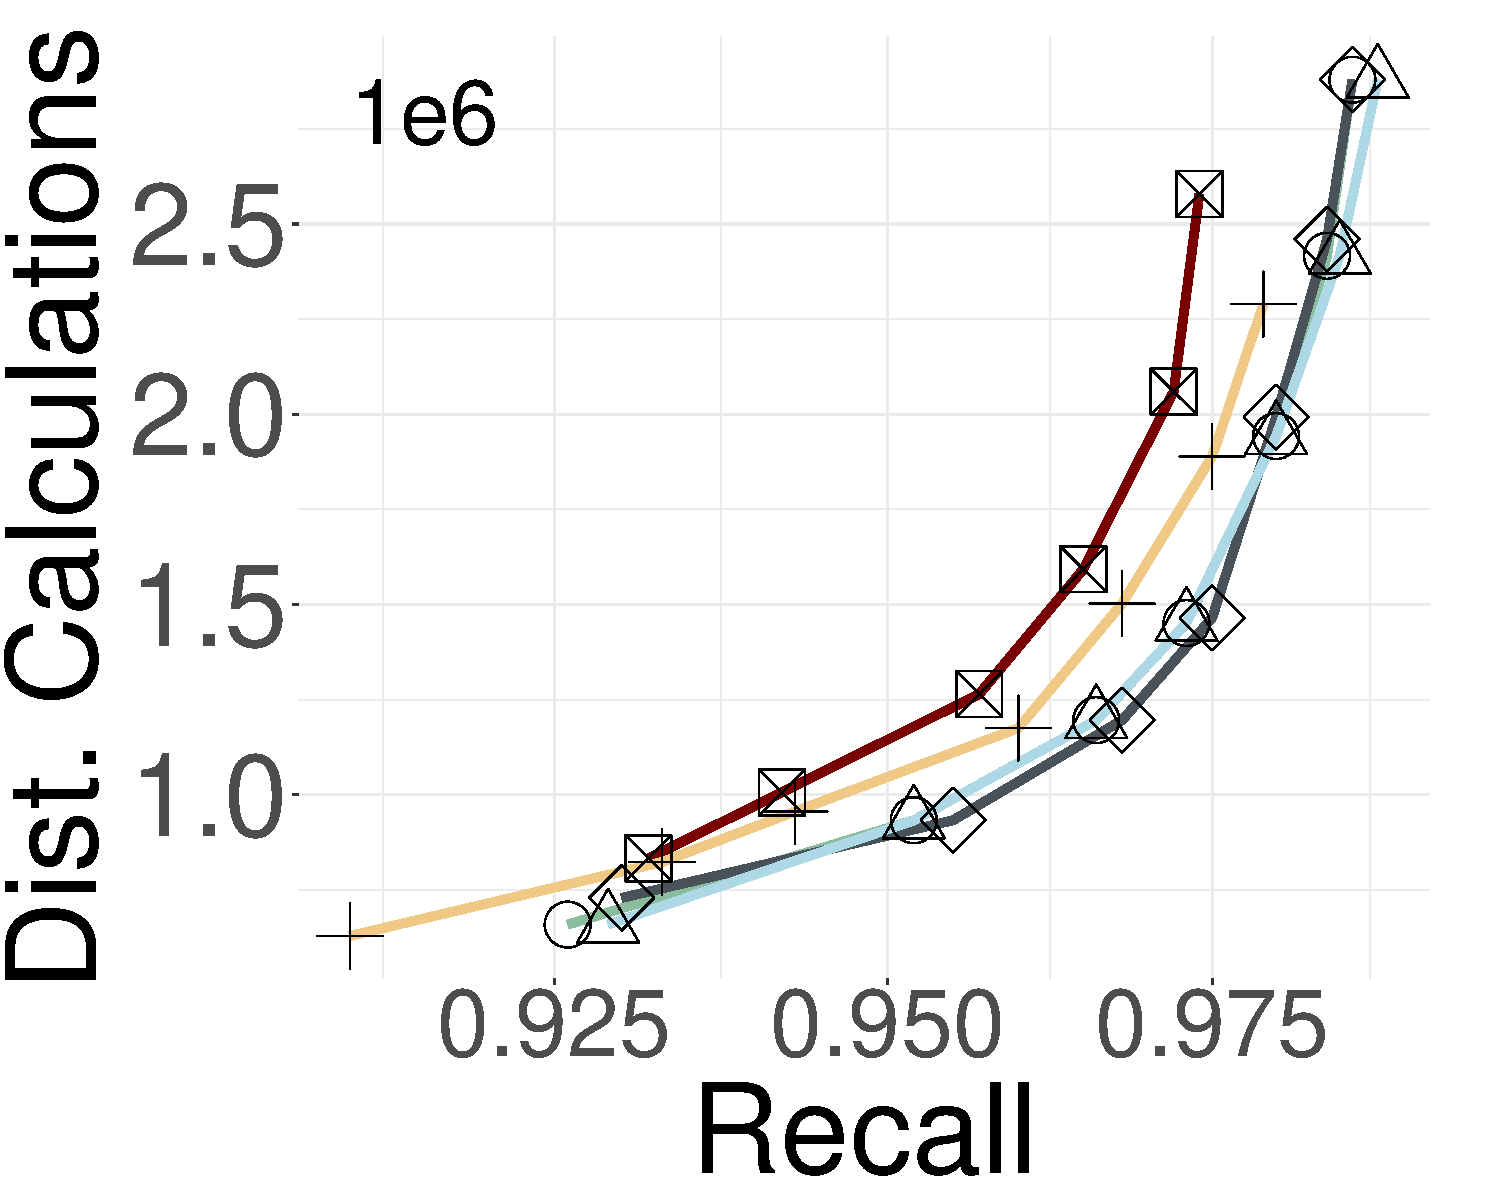
\includegraphics[width=\textwidth]{../img/oigas/RND_RRND/DC_SIFT1B.pdf}
   \caption{{Sift1B}}
		\label{fig:ND:sift1b}
		\end{subfigure}	
		\caption{{Combined RND\&RRND approach vs ND and NoND methods performance on real-world datasets}}
		\label{fig:ND:search:real}
 \end{figure}
 
For both the Deep and Sift datasets, combining RND and RRND enhances search performance for medium and smaller dataset sizes. This improvement is particularly evident in the 25GB datasets, where the combined approach outperforms existing Neighborhood Diversification (ND) methods that apply the same strategies. For larger datasets, extensive edge pruning becomes necessary as the path length to reach nearest neighbor (NN) regions increases, and pruning edges optimizes the number of comparisons required.

We integrate the combined diversification into OIGAS for small and medium-sized datasets. When the dataset size exceeds 100 million vectors, we employ RND pruning alone.

\subsection{Seed Selection}
We have previously analyzed and compared different strategies for seed selection (\ref{sec:experiments_ND_SS}). A key insight is that the optimal seed selection strategy depends on the dataset size. As demonstrated earlier, the Stacked NSW approach proposed by HNSW and K-random sampling of seed nodes have proven to deliver the best overall performance among various graph-based methods. Additionally, we found that for small and medium-sized datasets (\(< 100\)GB or approximately 260 million vectors), the K-random sampling approach yields the best performance. Figure~\ref{fig:snvskd} illustrates the difference in the number of distance calculations between the two scenarios, each adopting different seed selection methods: K-sampling and Stacked NSW. The difference is calculated as \(\text{NumDCs(SN)} - \text{NumDCs(KS)}\), where a positive value indicates that K-sampling is more efficient than Stacked NSW, and vice versa. For large datasets of 1 billion vectors, Stacked NSW emerges as the preferred choice. It is also worth noting that Stacked NSW requires building hierarchical multi-resolution NSW graphs during indexing, which incurs an additional time overhead during indexing. In contrast, K-random sampling can be executed during search without requiring extra structures.

\begin{figure}[tb] 
\centering
		\captionsetup{justification=centering}
		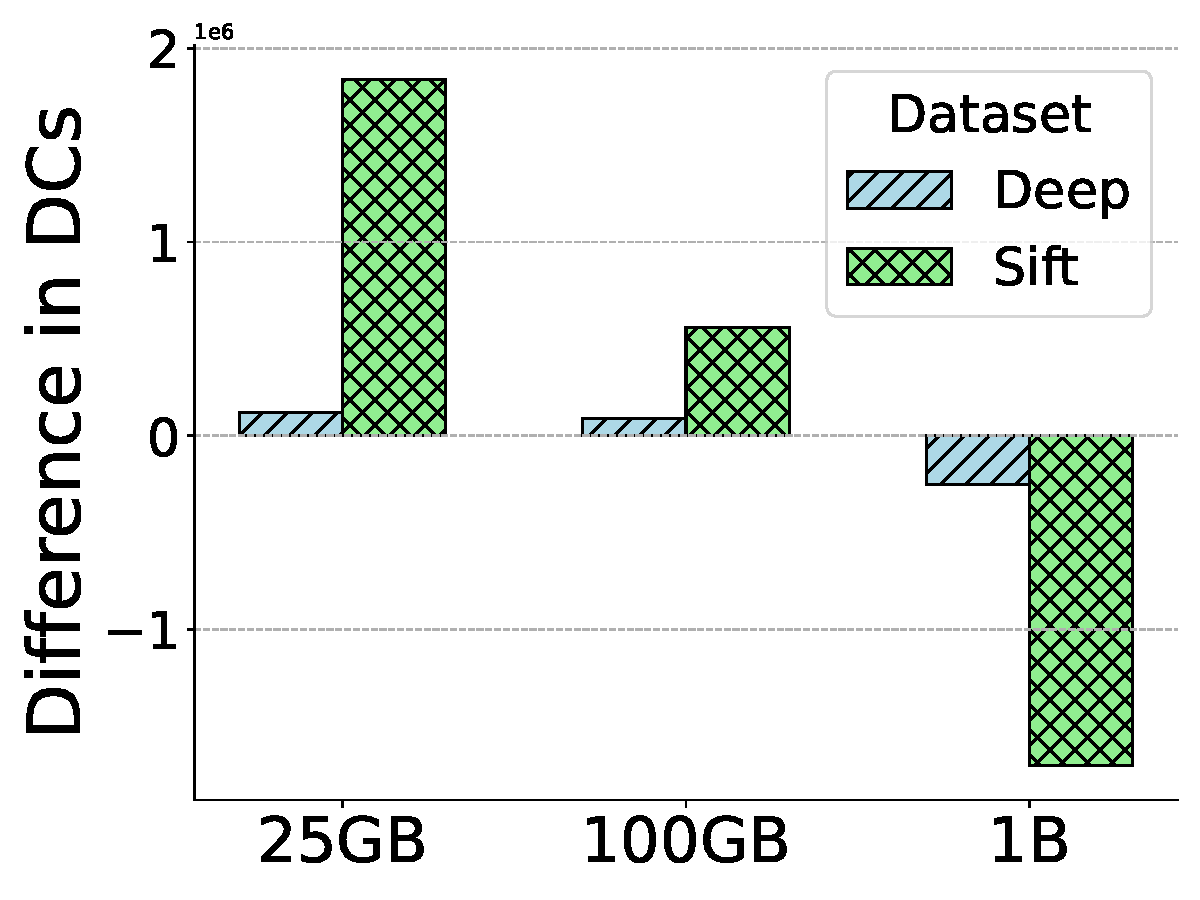
\includegraphics[width=0.4\columnwidth]{../img/oigas/SS/DC_SS.pdf}
		\caption{Difference in search efficiency using SN vs. KS for 0.99 recall search on different datasets and sizes}    
		\label{fig:snvskd}
 \end{figure}
 
In OIGAS, we adopt different strategies for seed selection, depending on the graph size. When the dataset size is smaller than billion scale (< 500M), we opt for K sampling in both indexing and search, while we keep the SNSW for billion scale datasets. Using K sampling has also shown a remarkable optimization in the number of computations during indexing as well. Figure~\ref{oigas:ss:impact} shows that using KS for seed selection reduces the number of distance calculations by millions for indexing a 1M dataset compared to using SN for seed selection (Fig.~\ref{oigas:ss:impact:dcs}). This difference grows to billions of distance calculations on the 25GB dataset, and can translate also into gains for queriers in both 1GB and 25GB (Fig. 7.10b) with saved computation and saved energy (Fig. 7.10c)
\begin{figure}[!htb]
\captionsetup{justification=centering}
	\centering

		\captionsetup{justification=centering}
		\captionsetup[subfigure]{justification=centering}
	\begin{subfigure}{0.3\textwidth}
		\includegraphics[width=\textwidth]{../img/oigas/SS/deepdcidxep.png}
		\caption{Difference in \#DCs} 
		\label{oigas:ss:impact:dcs}
		\end{subfigure}
  	\begin{subfigure}{0.3\textwidth}
		\includegraphics[width=\textwidth]{../img/oigas/SS/deepqrsidxep.png}
  	\label{oigas:ss:impact:qg}
		\caption{Query gains} 
		\label{fig:search:query:performance:25GB:hard:10p}
		\end{subfigure}
		\begin{subfigure}{0.3\textwidth}
		\includegraphics[width=\textwidth]{../img/oigas/SS/deepjidxep.pdf}
  	\label{oigas:ss:impact:joules}
		\caption{Energy Saved} 
		\label{fig:search:query:performance:25GB:hard:10p}
		\end{subfigure}
	\caption{Impact of the seed selection strategy during index building}
		\label{oigas:ss:impact}
	\end{figure}

\section{OIGAS}
We combined all efficient strategies discussed above-step-wise adaptive beam width, combined neighborhood diversification, KS seed selection and single priority queue beam search—into our new optimized incremental insertion based graph OIGAS. We compare OIGAS to the state-of-the-art incremental insertion-based method on a single graph, HNSW. We set the number of SWB steps to 12 and the RRND parameter $\alpha$ to 1.1 for the 25GB and 100GB datasets, and 1.05 for the 1B dataset size.

Note that in previous experimental studies in chapters ~\ref{chapter:graphfamily}, ~\ref{chapter:elpis} and ~\ref{chapter:elpis2}, we adopted single priority queue search for HNSW to fairly compare the method with state-of-the-art approaches. In the following experiments, we compare our optimized method with the original implementation of HNSW in the HNSWLib library~\cite{url/hnsw}.

\subsection{Indexing Performance}

The indexing time of OIGAS demonstrates remarkable efficiency over HNSW, notably due to the step-wise adaptive beam width.

Figure~\ref{fig:oigas_vs_hnsw_indexing} shows that the indexing time of OIGAS is up to 40\% faster than that of HNSW. The gap in indexing time can grow even larger with the increase of the necessary beam width. A high beam width may be required for challenging datasets, as each node needs highly accurate candidate nearest neighbors to effectively prune edges through neighborhood diversification.


\begin{figure}[htbp]
    \centering
    \captionsetup{justification=centering}
	\centering

		\captionsetup{justification=centering}
		\captionsetup[subfigure]{justification=centering}
        \begin{subfigure}[b]{\textwidth}
        \centering
 		\includegraphics[width=0.3\columnwidth]{../img/oigas/Search/legend.png}
    \end{subfigure}
    
            \begin{subfigure}[b]{0.3\textwidth}
            \centering
                \includegraphics[width=\textwidth]{../img/oigas/IDX/idx_time_deep_n.png}
                \caption{Deep1B}
        \label{fig:oigasidx:1Bdeep_Time}
    \end{subfigure}
    \hspace{0.4cm}
    \centering
             \begin{subfigure}[b]{0.3\textwidth}
                \includegraphics[width=\textwidth]{../img/oigas/IDX/idx_time_sift_n.png}
        \caption{Sift1B}
        \label{fig:oigasidx:1Bsift_Time}
    \end{subfigure}

    \caption{Indexing time}
    \label{fig:oigas_vs_hnsw_indexing}
\end{figure}

The memory footprint and index size of OIGAS remain comparable to those of HNSW. This is because OIGAS employs the maximum beam width in the final chunk of nodes, resulting in the same peak memory usage as HNSW when using the same indexing parameters \( M \) and \( \text{efConstruction} \).


\begin{figure}[htbp]
    \centering
    \captionsetup{justification=centering}
	\centering

		\captionsetup{justification=centering}
		\captionsetup[subfigure]{justification=centering}
        \begin{subfigure}[b]{\textwidth}
        \centering
 		\includegraphics[width=0.3\columnwidth]{../img/oigas/Search/legend.png}
    \end{subfigure}
    
            \begin{subfigure}[b]{0.3\textwidth}
            \centering
                \includegraphics[width=\textwidth]{../img/oigas/IDX/idx_footprint_deep_n.png}
                \caption{Deep1B}
        \label{fig:1M_Time}
    \end{subfigure}
    \hspace{0.4cm}
             \begin{subfigure}[b]{0.3\textwidth}
                \includegraphics[width=\textwidth]{../img/oigas/IDX/idx_footprint_sift_n.png}
        \caption{Sift1B}
        \label{fig:1B_Time}
    \end{subfigure}

    \caption{Indexing footprint}
    \label{fig:oigas:idx:time}
\end{figure}

\subsection{Search Performance}
In Figures ~\ref{fig:oigas:search},~\ref{fig:oigas:search:Large}, we can see that the search performance of OIGAS surpasses that of HNSW (as implemented in HNSWLib) across various datasets and scales. Approximately 90\% of this improvement is due to the use of a single priority queue for beam search rather than two priority queues.


\begin{figure}[ht]
    \centering
    \captionsetup{justification=centering}
	\centering

		\captionsetup{justification=centering}
		\captionsetup[subfigure]{justification=centering}
        \begin{subfigure}[b]{\textwidth}
        \centering
 		\includegraphics[width=0.3\columnwidth]{../img/oigas/Search/legend.png}
    \end{subfigure}

            \begin{subfigure}[b]{0.23\textwidth}
            \centering
                \includegraphics[width=\textwidth]{../img/oigas/Search/FINAL25GB/deep/Time.pdf}
                \caption{Deep}
        \label{fig:oigas:search:25:Deep}
    \end{subfigure}
            \begin{subfigure}[b]{0.23\textwidth}
            \centering
                \includegraphics[width=\textwidth]{../img/oigas/Search/FINAL25GB/sift/Time.pdf}
                \caption{Sift}
        \label{fig:oigas:search:25:Sift}
    \end{subfigure}
                        \begin{subfigure}[b]{0.23\textwidth}
            \centering
                \includegraphics[width=\textwidth]{../img/oigas/Search/FINAL25GB/sald/Time.pdf}
                \caption{Sald}
        \label{fig:oigas:search:25:sald}
    \end{subfigure}
            \begin{subfigure}[b]{0.23\textwidth}
            \centering
                \includegraphics[width=\textwidth]{../img/oigas/Search/FINAL25GB/seismic/Time.pdf}
                \caption{Seismic}
        \label{fig:oigas:search:25:Seismic}
    \end{subfigure}
    \caption{Search performance on 25GB datasets}
    \label{fig:oigas:search}
\end{figure}

\begin{figure}[ht]
    \centering
    \captionsetup{justification=centering}
	\centering

		\captionsetup{justification=centering}
		\captionsetup[subfigure]{justification=centering}
        \begin{subfigure}[b]{\textwidth}
        \centering
 		\includegraphics[width=0.3\columnwidth]{../img/oigas/Search/legend.png}
    \end{subfigure}
    
            \begin{subfigure}[b]{0.3\textwidth}
            \centering
                \includegraphics[width=\textwidth]{../img/oigas/Search/FINAL100GB/deep/Time.pdf}
                \caption{Deep100GB}
        \label{fig:oigas:search:100:Deep}
    \end{subfigure}
    \hspace{0.4cm}
            \begin{subfigure}[b]{0.3\textwidth}
            \centering
                \includegraphics[width=\textwidth]{../img/oigas/Search/FINAL1B/deep/Time.pdf}
                \caption{Deep1B}
        \label{fig:oigas:search:1B:Deep}
    \end{subfigure}

               \begin{subfigure}[b]{0.3\textwidth}
            \centering
                \includegraphics[width=\textwidth]{../img/oigas/Search/FINAL100GB/deep/Time.pdf}
                \caption{Sift100GB}
        \label{fig:oigas:search:100:Sift}
    \end{subfigure}
    \hspace{0.4cm}
            \begin{subfigure}[b]{0.3\textwidth}
            \centering
                \includegraphics[width=\textwidth]{../img/oigas/Search/FINAL1B/sift/Time.pdf}
                \caption{Sift1B}
        \label{fig:oigas:search:1B:Sift}
    \end{subfigure}
    \caption{Search performance on 100GB and 1B datasets}
    \label{fig:oigas:search:Large}
\end{figure}

We also optimized prefetching by tuning an offset parameter when prefetching neighbor vectors during the comparison of the query to the current node's neighbors. Instead of prefetching the immediate next neighbor in each iteration (i+1), we introduce a parameter offset\_pref such that we prefetch the neighbor at index ( i + 1 + offset\_pref ). We find that prefetching the second neighbor ( offset\_pref = 1 ) yields the best results for vectors of dimensions 96 and 128. This parameter depends on the cache size and the dimensionality of the vectors, as we must ensure that the prefetched vector is loaded into the cache before it is required for distance calculation, thereby preventing cache misses.

 
 \section{Conclusion}
In this chapter, we present our new insights and improvements to incremental insertion-based methods. We propose a new \textit{Optimized Incremental Insertion Graph-based Approximate vector Search} (OIGAS). This approach improves upon the popular incremental insertion-based graph, HNSW, by introducing a new method for efficient node insertion using \textit{Step-wise Adaptive Beam Width} (SWB). SWB optimizes indexing by up to 40\% in both indexing time for datasets up to 1B in size. This improvement can easily translate to hours or days of saved indexing time for billion-scale datasets. Furthermore, SWB's influence is not limited to indexing time; we also demonstrate how it improves graph search performance.

OIGAS incorporates other enhancements, namely combined Neighborhood Diversification (ND) that improves upon traditional use of single pruning strategy by employing a combined strategy for all nodes. OIGAS also adopts a simple yet efficient K-sampling strategy for seed selection during indexing and search on small and medium datasets, while still offering options such as SNSW for 1B-scale datasets. Additionally, it utilizes a single priority queue search over the double priority queue beam search used in HNSW. We further improve search efficiency by tuning the offset parameters for prefetching neighbor vectors, reducing cache misses. We have also observed that some techniques proposed by previous methods, such as using visited nodes as candidate neighbors set for nodes during indexing
%using Depth-First Search (DFS) to ensure connectivity or using visited nodes as candidate sets during neighborhood acquisition, 
do not lead to significant improvements.
